\pagenumbering{roman}
\section*{Resumen ejecutivo}
INFORMA UNSAAC formula un servicio de información institucional para la Escuela Profesional de Ingeniería Informática y de Sistemas. Integra gestión central de contenidos, consulta desde tres terminales táctiles de 55 pulgadas, continuidad por copia local, red local, videovigilancia de los equipos y un sistema de alimentación con respaldo y generación solar evaluada. La expansión a otras escuelas se organizará por edificios y resultados del piloto.

La necesidad es mejorar el acceso oportuno a avisos académicos, trámites, becas, eventos y oportunidades de colaboración. La población objetivo comprende 830 a 870 estudiantes matriculados en la EPIIS. La encuesta disponible comprende 300 respuestas de varias escuelas, 76 de la EPIIS: 81,7\% del conjunto declara haber omitido alguna fecha importante y 90,7\% expresa intención definitiva o probable de utilizar terminales. La finalidad se sustenta además en la Ley Universitaria, que obliga a publicar becas y servicios y exige equipos accesibles, y en los estándares de gestión de la información, recursos, bienestar y responsabilidad social del modelo de acreditación SINEACE 2025.

El servicio TI controla emisor, revisión, aprobación, vigencia, destinos y versión, con fuentes oficiales identificadas por tipo de aviso. Incluye consulta táctil y QR, cuentas por función, bloqueo de kiosco, supervisión, respaldo y recuperación. El requerimiento se redacta en diez especificaciones técnicas, ET-01 a ET-10, sin marca ni modelo, como dispone el Reglamento de la Ley N.° 32069. Cada valor se justifica frente a sus alternativas: tamaño de pantalla, memoria, almacenamiento, canales de grabación, disco, cable, puertos, servidor, inversor, batería y módulos. Las marcas sólo aparecen en cuadros comparativos que eligen una referencia de valorización con proveedores identificados.

La cota de diseño es 200 W por terminal, 12 horas de uso diario, 40 W de comunicaciones y videovigilancia y 15 W auxiliares. El escenario alcanza 8,52 kWh/día. Seis módulos de 615 Wp suman 3,69 kWp; con 4 HSP y factor 0,75 producen una referencia de 11,07 kWh/día. El inversor elegido admite 16 A por seguidor y opera hasta 4\,000 m; la batería de 4,8 kWh entrega 2,76 kWh de diseño para cuatro horas. Los conductores, protecciones, puesta a tierra y caídas de tensión se dimensionan con cálculo explícito.

Se comparan A0, mejora de canales existentes; A1, terminales y respaldo; y A2, servicio integral con generación FV. La inversión con reservas es S/ 9\,196,00, S/ 83\,392,94 y S/ 93\,523,38, respectivamente; el 60\% de la base de A2 procede de precios publicados. El costo de planificación a cinco años, con operación y reposición prevista, asciende a S/ 31\,996,00, S/ 128\,558,61 y S/ 135\,076,75. Con descuento al 8\%, el valor actual de costos es S/ 27\,402,76, S/ 118\,872,37 y S/ 126\,118,23. Con 850 estudiantes, el índice de costo-efectividad a cinco años es S/ 32,24, S/ 139,85 y S/ 148,37 por estudiante.

A1 presenta menor costo que A2 con el mismo objetivo de respaldo. La generación solar exige justificar un incremento inicial de S/ 10\,130,44, es decir S/ 8,52 por estudiante en valor actual, mediante desempeño energético y objetivos institucionales, además de financiamiento. La comparación permite ejecutar por etapas y evita atribuir a la energía beneficios que corresponden al servicio informático.

La ejecución se organiza en 16 semanas desde autorización y disponibilidad de recursos, con 408 horas-persona estimadas de servicios, compras y configuración en paralelo, puntos de aceptación y transferencia a operación. El mantenimiento se planifica por equipo, incluidas pantallas, cámaras, red y sistema FV. El cierre incorpora al menos 30 días de seguimiento, evaluación de indicadores, costos observados, lecciones y decisión de ampliar, ajustar o concluir.

\clearpage
\begingroup\small\setstretch{1.04}\setlength{\parskip}{0pt}\tableofcontents\endgroup
\clearpage
\begingroup\small\setstretch{1.04}\listoftables\endgroup
\clearpage
\begingroup\small\setstretch{1.04}\listoffigures\endgroup
\clearpage\pagenumbering{arabic}
\section{Problema}
\subsection{Contexto y delimitación de la necesidad}
La información de interés estudiantil se distribuye mediante grupos de mensajería, redes sociales, portales, correo y murales. La coexistencia de canales no constituye por sí misma una falla; la dificultad aparece cuando el usuario no identifica el aviso válido, lo encuentra tarde o debe consultar varios lugares para completar una misma gestión.

\subsection{Formulación del problema central}
El problema es el \textbf{acceso disperso y poco oportuno a información académica y administrativa relevante para la comunidad de la escuela}. La encuesta describe dependencia de medios informales, fechas importantes no conocidas a tiempo y valoración desfavorable del acceso a la información. Las fotografías muestran soportes físicos de difusión y las plantas permiten estudiar ubicaciones; no cuantifican por sí solas demoras o pérdidas de oportunidades.

\subsection{Causas, efectos y evidencia}
\cuadro{tab:problema}{Problema, causas y efectos por contrastar}{@{}P{3.0cm}Y Y@{}}{\textbf{Dimensión}&\textbf{Condición o causa propuesta}&\textbf{Efecto y verificación}}{
Origen de avisos & Publicaciones distribuidas entre canales con distinta autoridad & Dificultad para reconocer la versión válida; revisar avisos y fuentes\\*
Gestión editorial & Responsables, aprobación y caducidad por precisar & Riesgo de avisos atrasados o vencidos; verificar flujo de publicación\\
Acceso & Canales poco visibles o difíciles de localizar & Búsqueda adicional y fechas omitidas declaradas; observar consultas\\
Continuidad & Dependencia de red, alimentación y soporte & Riesgo de indisponibilidad; registrar incidencias y probar recuperación\\
Colaboración & Oportunidades y proyectos con visibilidad limitada & Interés en conectar equipos; comprobar uso efectivo\\
}
La línea base verificará tiempos de búsqueda, vigencia de avisos, responsables y disponibilidad. Estas variables permitirán contrastar las causas y medir el cambio del servicio.

\subsection{Árbol de problemas}
La figura \ref{fig:arbol_problemas} ordena las condiciones del cuadro \ref{tab:problema}. Las causas directas sostienen el problema central y éste produce efectos observables que convergen en un efecto final. Cada relación es una hipótesis de trabajo; la línea base verificará su magnitud.

\begin{center}
\begin{tikzpicture}[x=1cm,y=1cm,>=Latex,
  caja/.style={draw,rounded corners=3pt,align=center,inner sep=4pt,line width=0.6pt,font=\footnotesize,text width=2.52cm,minimum height=2.0cm,execute at begin node={\setstretch{1.0}\hyphenpenalty=10000\exhyphenpenalty=10000}},
  efecto/.style={caja,fill=unsaacrojo!7,draw=unsaacrojo!55},
  causa/.style={caja,fill=black!5,draw=black!40},
  central/.style={draw=unsaacrojo,fill=unsaacrojo,text=white,rounded corners=3pt,align=center,inner sep=5pt,font=\small\bfseries,text width=14.6cm,minimum height=1.5cm,execute at begin node={\setstretch{1.0}\hyphenpenalty=10000\exhyphenpenalty=10000}},
  final/.style={draw=unsaacrojo!70,fill=unsaacrojo!20,rounded corners=3pt,align=center,inner sep=4pt,line width=0.6pt,font=\footnotesize\bfseries,text width=14.6cm,minimum height=1.25cm,execute at begin node={\setstretch{1.0}\hyphenpenalty=10000\exhyphenpenalty=10000}},
  rotulo/.style={rotate=90,font=\scriptsize\bfseries,text=graytext,align=center},
  flecha/.style={->,draw=black!50,line width=0.7pt}]
\node[final] (fin) at (8.32,7.95) {Menor aprovechamiento de oportunidades académicas y profesionales, trámites y colaboración en la comunidad de la EPIIS};
\node[efecto] (e1) at (2.2,5.7) {Dificultad para reconocer el aviso válido};
\node[efecto] (e2) at (5.26,5.7) {Avisos atrasados o vencidos en circulación};
\node[efecto] (e3) at (8.32,5.7) {Búsqueda en varios canales y fechas omitidas\\[1pt]{\scriptsize\color{graytext}81,7\% las declara}};
\node[efecto] (e4) at (11.38,5.7) {Interrupciones de consulta sin recuperación};
\node[efecto] (e5) at (14.44,5.7) {Baja visibilidad de proyectos y oportunidades};
\node[central] (pc) at (8.32,3.35) {Acceso disperso y poco oportuno a información académica y administrativa relevante para la comunidad de la EPIIS};
\node[causa] (c1) at (2.2,1.0) {Canales con distinta autoridad\\[1pt]{\scriptsize\color{graytext}79,3\% WhatsApp o Facebook}};
\node[causa] (c2) at (5.26,1.0) {Sin responsables, aprobación ni caducidad definidos};
\node[causa] (c3) at (8.32,1.0) {Consulta poco visible en espacios comunes};
\node[causa] (c4) at (11.38,1.0) {Acceso dependiente de red, energía y soporte};
\node[causa] (c5) at (14.44,1.0) {Proyectos y oportunidades sin canal de difusión};
\foreach \n in {1,...,5}{
  \draw[flecha] (c\n.north) -- (c\n.north |- pc.south);
  \draw[flecha] (e\n.south |- pc.north) -- (e\n.south);
  \draw[flecha] (e\n.north) -- (e\n.north |- fin.south);
}
\node[rotulo] at (0.35,7.95) {EFECTO\\FINAL};
\node[rotulo] at (0.35,5.7) {EFECTOS};
\node[rotulo] at (0.35,3.35) {PROBLEMA};
\node[rotulo] at (0.35,1.0) {CAUSAS};
\end{tikzpicture}
\captionof{figure}{Árbol de problemas del servicio de información de la EPIIS}\label{fig:arbol_problemas}
\end{center}

\subsection{Entorno de difusión}
Los soportes físicos de información forman parte del entorno que atenderá el servicio. El piloto integrará avisos de estos canales con publicaciones digitales y una gestión común de vigencia.
% Las tres fotografías comparten una fila para que la figura no se divida entre páginas.
\par\vspace{4pt}\noindent\begin{minipage}{\linewidth}\centering
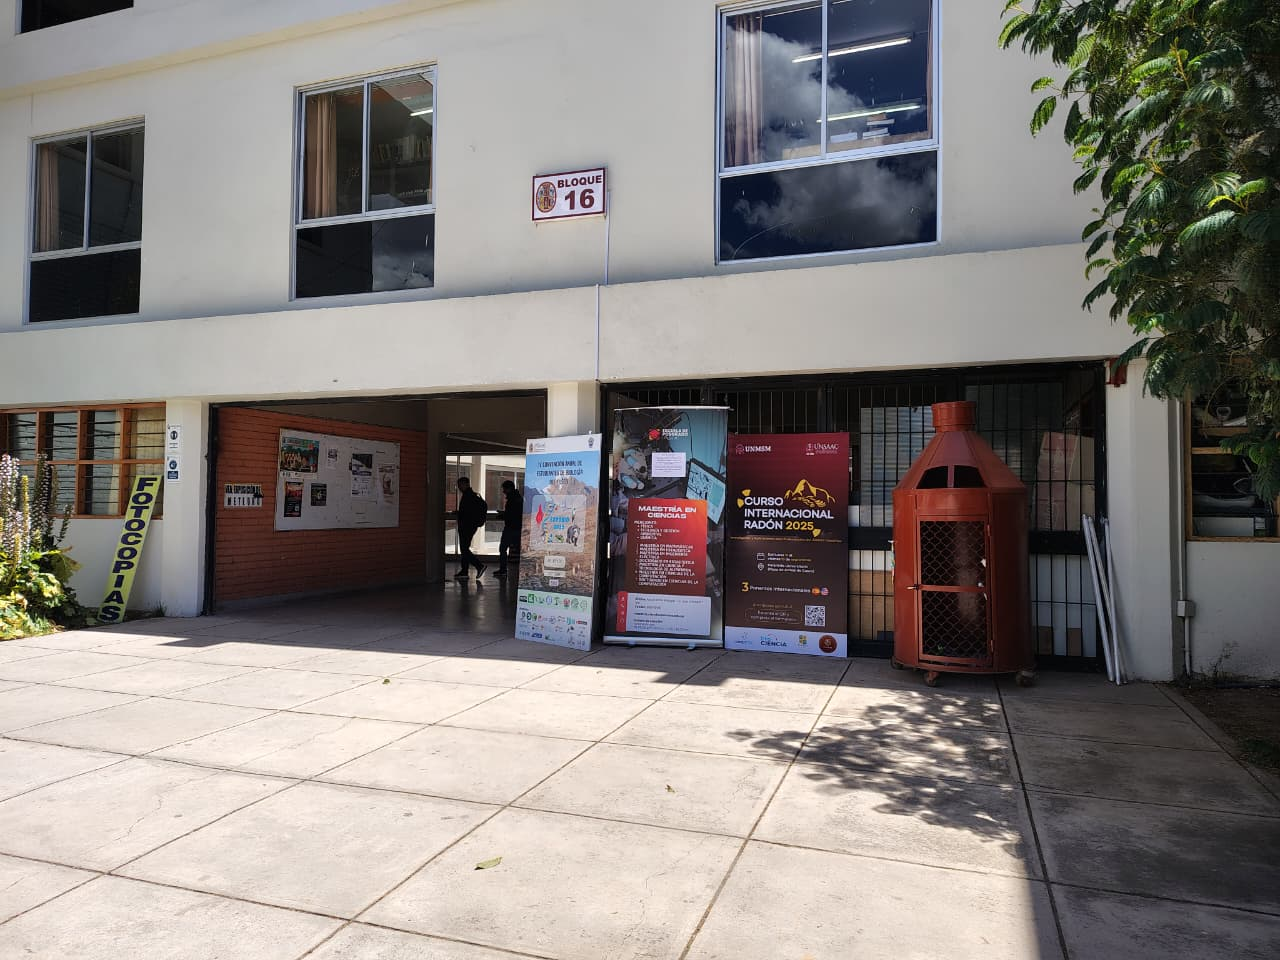
\includegraphics[height=4.4cm,keepaspectratio]{imagenes/foto_ingreso.png}\hfill
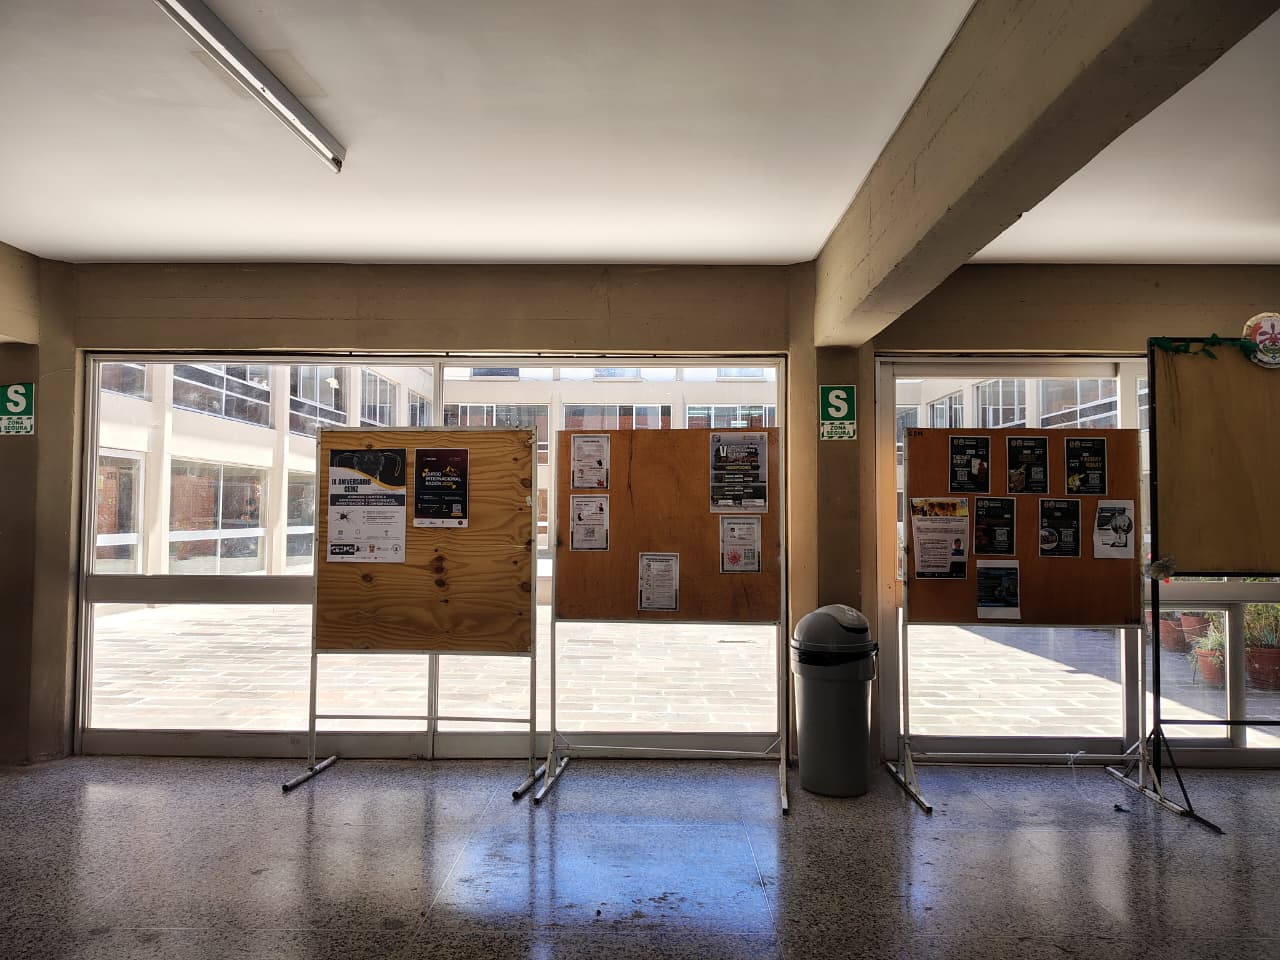
\includegraphics[height=4.4cm,keepaspectratio]{imagenes/foto_murales.png}\hfill
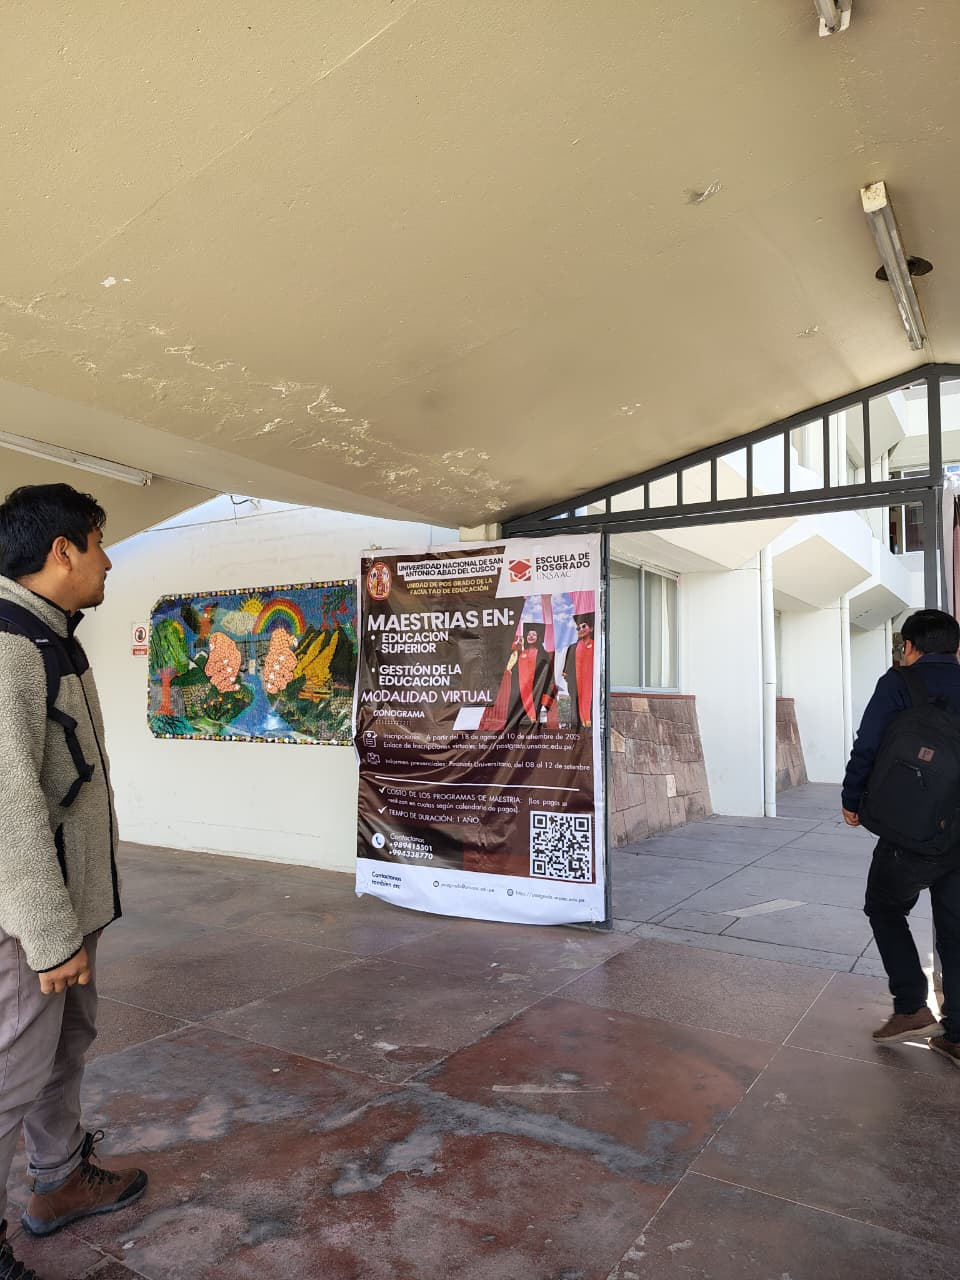
\includegraphics[height=4.4cm,keepaspectratio]{imagenes/foto_pasillo.png}\par
\captionof{figure}{Entorno de difusión: ingreso, murales y pasillos}\label{fig:entorno}
\end{minipage}\par\vspace{4pt}

\section{Origen del proyecto}
La iniciativa se origina en la necesidad de articular la información que llega a la comunidad estudiantil por distintos medios y convertirla en un servicio de consulta confiable. Las respuestas sobre fechas omitidas, acceso a avisos y formatos preferidos orientan esa necesidad; no demuestran que una tecnología particular sea la única respuesta.

El componente informático surge de la oportunidad de gestionar el ciclo completo del aviso: emisor, validación, publicación, vigencia, destino y seguimiento. La consulta táctil y el QR se plantean como alternativas complementarias para acceder a esa información desde espacios comunes y dispositivos personales.

El componente solar se evalúa por aporte energético, continuidad y costo de ciclo de vida. Su incorporación exige comparar el servicio con respaldo de red y la variante con generación FV, bajo iguales funciones y objetivos de disponibilidad.

Los porcentajes del cuadro \ref{tab:origen} corresponden a la base gráfica de \textbf{300 respuestas de varias escuelas}, de las cuales 76 pertenecen a Ingeniería Informática y de Sistemas. No se dispone de cruces individuales para calcular esos resultados sólo para la EPIIS; por tanto, describen al conjunto de respuestas y orientan la validación local.

\cuadro{tab:origen}{Origen y fundamento de las decisiones de diseño}{@{}P{3.1cm}Y Y@{}}{\textbf{Necesidad o condición}&\textbf{Evidencia disponible}&\textbf{Decisión propuesta}}{
Acceso oportuno & 81,7\% declara haber omitido alguna fecha por falta de información & Centralizar avisos y validar el tiempo de consulta\\*
Fuente reconocible & 79,3\% usa principalmente WhatsApp o Facebook & Mostrar emisor, fuente oficial, revisión y vigencia\\
Consulta accesible & Preferencias táctil 60,7\% y QR 31,7\% & Probar terminales y continuidad en móvil; conservar otros canales\\
Gestión de contenidos & Riesgo de duplicidad y desactualización por contrastar & Establecer responsables y flujo editorial antes de automatizar\\
Aporte y respaldo energético & Cargas y condiciones del sitio pendientes & Comparar red/respaldo con FV híbrida dimensionada\\
}

\section{Finalidad pública}

El proyecto busca facilitar a la comunidad de la EPIIS el acceso a información institucional oportuna, verificable y comprensible. Se concentra en oportunidades académicas y profesionales, fechas de trámites, eventos y proyectos de colaboración. Un servicio bien gestionado puede reducir búsquedas innecesarias y ampliar la visibilidad de oportunidades, sin sustituir los canales oficiales ni limitar el acceso de quienes no se encuentren en el pabellón.

La intervención integra proceso editorial, software, terminales públicos, conectividad y alimentación eléctrica. La utilidad pública reside en que el usuario encuentre información válida y pueda actuar sobre ella. La pantalla y el sistema solar son medios para prestar ese servicio, cuya conveniencia se evaluará con resultados medibles y recursos sostenibles.

El ámbito inicial comprende tres ubicaciones interiores de la EPIIS, una por piso. La expansión se organizará por edificios después de evaluar resultados del piloto, infraestructura y capacidad de contenido y soporte.

\subsection{Sustento normativo y exigencias de calidad}
La finalidad no descansa sólo en la preferencia de los usuarios. El cuadro \ref{tab:normativa} relaciona las obligaciones legales y los estándares de acreditación con lo que el servicio debe cumplir. Los artículos citados de la Ley Universitaria se verificaron en su texto publicado \cite{ley30220}; los estándares corresponden al modelo de acreditación de programas universitarios del SINEACE aprobado en 2025 \cite{sineace2025}.

\cuadro{tab:normativa}{Sustento normativo y de acreditación del servicio}{@{}P{3.3cm}Y Y@{}}{\textbf{Norma o estándar}&\textbf{Disposición pertinente}&\textbf{Exigencia para el proyecto}}{
Ley N.° 30220, art. 11 & Publicar en forma permanente y actualizada, entre otros, becas y créditos disponibles (11.4) y número de alumnos por programa (11.8) & Difundir avisos oficiales con fuente y vigencia, y enlazar al portal de transparencia\\*
Ley N.° 30220, art. 100 & Ambientes y equipos accesibles para personas con discapacidad (100.8); uso de los servicios académicos y de bienestar (100.10) & Altura, aproximación, contraste y alternativa QR; consulta libre y gratuita\\
Ley N.° 30220, art. 126 & Programas de bienestar para la comunidad universitaria & Difundir becas, salud, eventos y servicios de apoyo\\
SINEACE 2025, estándares 5 y 8 & Recursos e infraestructura tecnológica; gestión de la información para decidir y mejorar & Registros de uso, vigencia y desempeño exportables como evidencia\\
SINEACE 2025, estándares 6 y 7 & Responsabilidad social y desarrollo sostenible; bienestar y servicios de apoyo & Medición del aporte FV y difusión de servicios estudiantiles\\
Ley N.° 32069 y su Reglamento, num. 44.6 & El requerimiento no menciona marca, fabricante ni procedencia, salvo compatibilización aprobada & Especificaciones genéricas ET-01 a ET-10; marcas sólo en la indagación\\
Ley N.° 29733 y D.S. N.° 016-2024-JUS & Tratamiento de datos personales y videovigilancia & Consulta sin datos personales; cámaras con aviso, finalidad y conservación limitadas\\
CNE, Utilización & Seguridad de instalaciones eléctricas interiores & Protecciones, tierra y caída de tensión verificadas por profesional\\
Régimen RAEE & Gestión de residuos de aparatos eléctricos y electrónicos & Retiro trazable de equipos y baterías\\
}
Las normas y estándares se citan en \cite{contrataciones,compatibilizacion,datos,cne,raee}. La universidad no tiene equipamiento previo de este tipo que justifique una compatibilización. Por ello el requerimiento se redacta por desempeño y cualquier marca que cumpla la especificación puede ofertar.

\subsection{Estadísticas e insumos de la formulación}
Cada cifra que usa el informe proviene de una fuente identificada. El cuadro \ref{tab:insumos} reúne los insumos que determinan alcance, demanda, energía y costo, e indica cómo se reemplazarán cuando exista el dato institucional.

\cuadro{tab:insumos}{Estadísticas e insumos utilizados y su fuente}{@{}P{3.4cm}P{3.0cm}Y@{}}{\textbf{Insumo}&\textbf{Valor}&\textbf{Fuente y actualización}}{
Estudiantes de la EPIIS & 830 a 870 & Matrícula referencial del equipo; confirmar con registro oficial 2026-II\\*
Respuestas de la encuesta & 300; 76 de la EPIIS & Base gráfica del instrumento, anexo A\\
Fechas omitidas por falta de información & 81,7\% & Encuesta, pregunta 4\\
Uso principal de mensajería y redes & 79,3\% & Encuesta, pregunta 3\\
Intención favorable de uso & 90,7\% & Encuesta, pregunta 6\\
Radiación horizontal media & 4,83 kWh/m\textsuperscript{2}/día; mínimo 4,10 & NASA POWER 2021 a 2025 \cite{nasa}\\
Horas de servicio y días de uso & 12 h/día; 200 días/año & Supuesto de calendario académico; ajustar con horario aprobado\\
Tarifa eléctrica & S/ 0,80/kWh & Supuesto; reemplazar con el pliego vigente de Electro Sur Este y el recibo institucional \cite{pliego}\\
Tipo de cambio & S/ 3,457 por dólar & BCRP, SBS venta, 9 de octubre de 2026 \cite{bcrp}\\
Impuesto General a las Ventas & 18\% & SUNAT \cite{igv}\\
Tasa social de descuento & 8\% & MEF, parámetros de evaluación social \cite{mefparametros}\\
Precios de equipos & 30 de octubre de 2026 & Proveedores identificados; secciones \ref{sec:mercado} y \ref{sec:seleccion}\\
}

\section{Antecedentes}
\subsection{Experiencias y criterio de adaptación}
La señalización digital institucional permite coordinar mensajes y destinos bajo una administración común. El servicio de la Universidad de Michigan ilustra la gestión de contenidos, publicación y soporte mediante funciones definidas \cite{michigan}. Su adaptación al proyecto prioriza responsabilidades editoriales, distribución y atención de incidencias.

Los dispositivos interactivos para docencia y los tótems informativos cumplen usos distintos. Este proyecto se concentra en consulta breve y difusión en espacios comunes. Una pizarra de aula no acredita las características ni el consumo de un terminal vertical completo.

La mejora tecnológica deberá acompañarse de emisores autorizados, revisión de avisos, responsables de caducidad y atención de incidencias. De lo contrario, una publicación dispersa o desactualizada sólo cambiaría de soporte.

\subsection{Interesados}
\cuadro{tab:interesados}{Interesados y participación necesaria}{@{}P{3.0cm}Y Y@{}}{\textbf{Interesado}&\textbf{Necesidad}&\textbf{Participación prevista}}{
Estudiantes y docentes & Encontrar oportunidades y avisos pertinentes & Validar categorías, ubicación y consulta\\*
Personal y emisores de escuela & Publicar y retirar información autorizada & Definir fuentes, revisión y responsables\\
Dirección de escuela & Servicio útil y sostenible & Priorizar alcance y gestionar autorizaciones\\
Área TI competente & Seguridad, integración y soporte & Validar red, alojamiento, cuentas y recuperación\\
Infraestructura y especialistas & Instalación segura y compatible & Revisar cubierta, anclajes, circuitos y sistema FV\\
Administración institucional & Costo completo y compra sustentada & Revisar financiamiento, ofertas y procedimiento aplicable\\
}
La dirección de escuela coordinará la designación de responsables editoriales, de TI y de infraestructura antes de la puesta en servicio.

\section{Objetivos}
\subsection{Árbol de objetivos}
El árbol de objetivos de la figura \ref{fig:arbol_objetivos} transforma cada causa en un medio y cada efecto en un fin. Los medios 1, 2 y 5 se atienden con el objetivo específico 1; el medio 3, con el 2; el medio 4, con los objetivos 3 y 4. El objetivo 5 evalúa el conjunto antes de ampliar.

\begin{center}
\begin{tikzpicture}[x=1cm,y=1cm,>=Latex,
  caja/.style={draw,rounded corners=3pt,align=center,inner sep=4pt,line width=0.6pt,font=\footnotesize,text width=2.52cm,minimum height=2.0cm,execute at begin node={\setstretch{1.0}\hyphenpenalty=10000\exhyphenpenalty=10000}},
  fines/.style={caja,fill=tiazul!7,draw=tiazul!55},
  medio/.style={caja,fill=verdeprueba!9,draw=verdeprueba!60},
  central/.style={draw=tiazul,fill=tiazul,text=white,rounded corners=3pt,align=center,inner sep=5pt,font=\small\bfseries,text width=14.6cm,minimum height=1.5cm,execute at begin node={\setstretch{1.0}\hyphenpenalty=10000\exhyphenpenalty=10000}},
  final/.style={draw=tiazul!70,fill=tiazul!20,rounded corners=3pt,align=center,inner sep=4pt,line width=0.6pt,font=\footnotesize\bfseries,text width=14.6cm,minimum height=1.25cm,execute at begin node={\setstretch{1.0}\hyphenpenalty=10000\exhyphenpenalty=10000}},
  rotulo/.style={rotate=90,font=\scriptsize\bfseries,text=graytext,align=center},
  etiqueta/.style={font=\scriptsize\bfseries,text=verdeprueba,inner sep=1pt},
  flecha/.style={->,draw=black!50,line width=0.7pt}]
\node[final] (fin) at (8.32,7.95) {Mayor aprovechamiento de oportunidades académicas y profesionales, trámites y colaboración en la comunidad de la EPIIS};
\node[fines] (e1) at (2.2,5.7) {Aviso válido reconocible por su fuente y emisor};
\node[fines] (e2) at (5.26,5.7) {Avisos vigentes y retirados a tiempo};
\node[fines] (e3) at (8.32,5.7) {Consulta rápida y fechas atendidas a tiempo};
\node[fines] (e4) at (11.38,5.7) {Consulta disponible ante cortes de red o energía};
\node[fines] (e5) at (14.44,5.7) {Proyectos y oportunidades visibles para formar equipos};
\node[central] (pc) at (8.32,3.35) {Acceso oportuno y confiable a información académica y administrativa relevante para la comunidad de la EPIIS};
\node[medio] (c1) at (2.2,1.0) {Fuente oficial centralizada con emisor visible};
\node[medio] (c2) at (5.26,1.0) {Flujo editorial con responsables, aprobación y caducidad};
\node[medio] (c3) at (8.32,1.0) {Tres terminales táctiles y QR en espacios comunes};
\node[medio] (c4) at (11.38,1.0) {Copia local, respaldo eléctrico y generación FV};
\node[medio] (c5) at (14.44,1.0) {Difusión autorizada de proyectos de colaboración};
\foreach \n/\oe in {1/OE1,2/OE1,3/OE2,4/{OE3 y OE4},5/OE1}{
  \draw[flecha] (c\n.north) -- (c\n.north |- pc.south);
  \draw[flecha] (e\n.south |- pc.north) -- (e\n.south);
  \draw[flecha] (e\n.north) -- (e\n.north |- fin.south);
  \node[etiqueta,anchor=north] at (c\n.south) {Medio \n\ $\cdot$ \oe};
}
\node[rotulo] at (0.35,7.95) {FIN\\ÚLTIMO};
\node[rotulo] at (0.35,5.7) {FINES};
\node[rotulo] at (0.35,3.35) {OBJETIVO};
\node[rotulo] at (0.35,1.0) {MEDIOS};
\end{tikzpicture}
\captionof{figure}{Árbol de objetivos: medios y fines del proyecto}\label{fig:arbol_objetivos}
\end{center}

\subsection{Objetivo general}
Mejorar el acceso oportuno a información institucional y oportunidades de colaboración de la EPIIS mediante un servicio integrado de contenidos y consulta interactiva, con alimentación solar híbrida evaluada y condiciones verificables para su futura expansión en la UNSAAC.

\subsection{Objetivos específicos}
\begin{enumerate}
\item Centralizar avisos, identificando emisor, fuente, vigencia, destinatarios y responsable de revisión.
\item Facilitar la consulta desde tres terminales interiores y códigos QR que permitan continuar la lectura en dispositivos personales.
\item Asegurar publicación controlada, continuidad de consulta, supervisión y recuperación mediante pruebas del conjunto.
\item Dimensionar el aporte FV y el respaldo a partir de cargas, horario, condiciones del sitio y costo total.
\item Evaluar utilidad, operación y costos del piloto antes de aprobar una ampliación institucional.
\end{enumerate}

\cuadro{tab:indicadores}{Indicadores y metas iniciales de aceptación}{@{}P{2.8cm}Y P{3.8cm}@{}}{\textbf{Indicador}&\textbf{Medición}&\textbf{Meta propuesta}}{
Vigencia editorial & Avisos con fuente, responsable, inicio y vencimiento entre total revisado & 100\% del conjunto del ensayo\\*
Consulta exitosa & Participantes que localizan un aviso y abren su detalle & Al menos 90\% en casos y muestra documentados\\
Tiempo de búsqueda & Mediana de tiempo en tareas equivalentes antes y durante el piloto & Reducción objetivo 30\%; línea base por levantar\\
Sincronización & Desde publicación aprobada hasta versión aplicada en terminal conectado & Hasta 5 minutos en ensayo\\
Continuidad local & Consulta válida tras corte de red y reinicio & Recuperar consulta en las tres terminales\\
Autonomía eléctrica & Horas con cargas críticas durante corte controlado & Objetivo 4 h; carga y condiciones verificadas\\
Aporte solar & kWh FV aprovechados, kWh de red y energía de cargas & Medir al menos 30 días; meta final tras estudio del recurso\\
}
Las metas de aceptación se contrastarán con una línea base y un protocolo de evaluación con usuarios. El seguimiento medirá consulta efectiva, además de la intención de uso expresada en la encuesta.

\subsection{Matriz de marco lógico}
El cuadro \ref{tab:mml} integra el árbol de objetivos, los indicadores y los supuestos externos. Los componentes se acreditan con los entregables E4 a E6 y las actividades corresponden a los paquetes W1 a W7 desarrollados en la ejecución. Los códigos PF, PC y PE remiten a los casos del plan de pruebas.

% Matriz extensa: admite continuar en la página siguiente con encabezado repetido.
% longtable incrementa el contador de cuadros por sí mismo; se compensa al cerrar.
\par
\begingroup\footnotesize\setstretch{1.0}\renewcommand{\arraystretch}{1.1}\setlength{\tabcolsep}{3.5pt}\setlength{\LTpre}{0pt}
\captionof{table}{Matriz de marco lógico del piloto}\label{tab:mml}\nopagebreak
\begin{xltabular}{\linewidth}{@{}P{1.95cm}YYYY@{}}
\toprule\textbf{Nivel}&\textbf{Resumen narrativo}&\textbf{Indicadores}&\textbf{Medios de verificación}&\textbf{Supuestos}\\\midrule
\endfirsthead
\multicolumn{5}{@{}l}{\emph{Continuación del cuadro \ref{tab:mml}}}\\\toprule
\textbf{Nivel}&\textbf{Resumen narrativo}&\textbf{Indicadores}&\textbf{Medios de verificación}&\textbf{Supuestos}\\\midrule
\endhead
\bottomrule
\endfoot
\bottomrule
\endlastfoot
\textbf{Fin} & Mayor aprovechamiento de oportunidades académicas y profesionales, trámites y colaboración en la EPIIS & Proporción que declara haber omitido fechas por falta de información; 81,7\% en la encuesta del conjunto, meta tras la línea base & Encuesta de seguimiento con el mismo instrumento; informe de evaluación G6 & La escuela mantiene la publicación centralizada después del piloto\\*\midrule
\textbf{Propósito} & Los 830 a 870 estudiantes de la EPIIS acceden de forma oportuna a información válida y vigente & Consulta exitosa de al menos 90\%; reducción de 30\% en la mediana del tiempo de búsqueda & Línea base y pruebas con usuarios; panel de resultados del piloto & Los emisores publican por el canal centralizado y la comunidad conoce el servicio\\\midrule
\textbf{C1.} Gestión editorial & CMS con borrador, revisión, aprobación, vigencia y destinos configurado & 100\% de avisos con fuente, responsable y vigencia; publicación aplicada en hasta 5 min & Casos PF1 a PF5; registro de auditoría del CMS & Responsables editoriales designados y capacitados\\\midrule
\textbf{C2.} Consulta táctil y QR & Tres terminales de 55 pulgadas en modo kiosco, una por piso, con QR para continuar en móvil & Detalle en hasta 3 s en 95\% de intentos; consulta recuperada tras corte y reinicio & Casos PC1 a PC5 y ensayo de capacidad; acta G4 & Suministro conforme al término de la semana 6 y red institucional disponible\\\midrule
\textbf{C3.} Alimentación y seguridad & Circuito de cargas críticas con inversor híbrido, banco de 4,8 kWh, 3,69 kWp FV y videovigilancia de los terminales & Cuatro horas de autonomía en ensayo; aporte FV medido durante al menos 30 días; 30 días de grabación & Casos PE1 a PE5 y PC6; registros del medidor, del monitoreo y del NVR & Cubierta apta y conexión autorizada por la institución\\\midrule
\textbf{C4.} Operación y evaluación & Responsables capacitados, expediente transferido y piloto evaluado & Disponibilidad de consulta de al menos 98\% por terminal; decisión G6 registrada & Expediente de transferencia; informe de evaluación y cierre & La institución financia la operación y mantiene a los responsables\\\midrule
\textbf{Actividades} & W1 a W7: ingeniería, CMS, interfaz, instalación, pruebas, transferencia y coordinación en 16 semanas & 408 HP; inversión A2 de S/ 93\,284,93 con reservas; puertas G0 a G5 aprobadas & Cronograma, control de costos y actas de las puertas de avance & Autorización, responsables y financiamiento disponibles en G0\\
\end{xltabular}\addtocounter{table}{-1}\par\endgroup

\section{Estudio de mercado}\label{sec:mercado}
\subsection{Diseño de la investigación y base de análisis}
Se estudian las \textbf{necesidades de usuarios} y la \textbf{oferta tecnológica y comercial}. La base gráfica de la encuesta comprende \textbf{300 respuestas}; 76 corresponden a Ingeniería Informática y de Sistemas y el resto a otras escuelas. La fecha de aplicación, el método de selección y los registros individuales no están disponibles. Por ello se utiliza como evidencia descriptiva del conjunto, con análisis actualizado en 2026.

El anexo A presenta el instrumento y los resultados complementarios. Para estimar la magnitud específica de la necesidad en la EPIIS se realizará la validación local prevista en el plan.

\subsection{Fuentes de información y método de recopilación}
La información del informe se obtuvo de fuentes primarias y secundarias. El cuadro \ref{tab:fuentes_info} indica qué dato aporta cada una, cómo se recopiló y con qué límite se usa. Las páginas comerciales se consultaron el 30 de octubre de 2026 y su procedencia se registra en el anexo C.

\cuadro{tab:fuentes_info}{Fuentes de información y método de recopilación}{@{}P{3.0cm}Y Y@{}}{\textbf{Fuente}&\textbf{Dato obtenido y método}&\textbf{Uso y límite}}{
Encuesta a estudiantes & 300 respuestas a diez preguntas cerradas; gráficos del instrumento & Necesidad declarada; no reemplaza la línea base\\*
Fotografías y planos & Registro del entorno y de las tres ubicaciones propuestas & Emplazamiento; se verificará en el levantamiento\\
Normas y estándares & Lectura del texto publicado de leyes, reglamento y modelo de acreditación & Obligaciones y criterios de aceptación\\
Fichas de fabricantes & Datos técnicos de cada modelo comparado, en PDF o en la página del producto & Cumplimiento de ET-01 a ET-10; prevalece sobre la publicidad\\
Páginas de proveedores & Precio, IGV, stock, garantía y enlace, con RUC cuando se publica & Valor referencial; requiere cotización formal\\
Datos abiertos & Serie NASA POWER y tipo de cambio del BCRP & Recurso solar y conversión de importes en dólares\\
Documentación de software & Funciones, licencias y almacenamiento del CMS y de los reproductores & Ruta de software y pruebas del cliente\\
Estimación propia & Horas-persona, tarifas, metrados y supuestos explícitos & Planificación; se reemplazará con ofertas y diseño\\
}

\subsection{Población de referencia, potencial y objetivo}
Según la información de matrícula disponible para el equipo, la EPIIS cuenta con \textbf{830 a 870 estudiantes por semestre}; la cifra exacta se tomará del registro oficial de matrícula de 2026-II. El servicio es de acceso libre en los tres pisos y continúa por QR, por lo que no excluye grupos dentro de la escuela. Docentes, personal y visitantes también lo utilizarán, pero no se cuantifican hasta levantar la línea base; su exclusión hace conservador el indicador por estudiante.

\cuadro{tab:poblacion}{Población de referencia, potencial y objetivo}{@{}P{2.6cm}Y P{3.4cm}@{}}{\textbf{Población}&\textbf{Definición}&\textbf{Magnitud}}{
Referencia & Comunidad que transita por el pabellón de la EPIIS: estudiantes, docentes, personal administrativo y visitantes & Estudiantes: 830 a 870; demás grupos por registrar\\*
Potencial & Estudiantes matriculados en la EPIIS que requieren avisos académicos, trámites, becas, eventos y oportunidades & 830 a 870 por semestre\\
Objetivo & Estudiantes matriculados atendidos por el piloto mediante tres terminales, una por piso, y consulta móvil por QR & 830 a 870; valor central 850\\
Usuarios probables & Población objetivo por la intención favorable del conjunto encuestado, 90,7\%; sensibilidad, no meta & 753 a 789\\
}
Con el valor central, cada terminal atiende en promedio unos 283 estudiantes. La intención de uso proviene del conjunto de 300 respuestas, por lo que los usuarios probables sólo ilustran una sensibilidad; el uso real se medirá durante el seguimiento del piloto.

\cuadro{tab:ficha_encuesta}{Ficha técnica de la encuesta disponible}{@{}P{3.4cm}Y@{}}{\textbf{Elemento}&\textbf{Descripción}}{
Unidad de análisis & Estudiante de la UNSAAC que respondió el cuestionario\\*
Instrumento & Cuestionario de diez preguntas cerradas; el anexo A presenta su contenido\\
Respuestas & 300 de varias escuelas; 76 de Ingeniería Informática y de Sistemas\\
Cobertura en la EPIIS & 76 respuestas frente a 830 a 870 estudiantes: 8,7\% a 9,2\%\\
Fecha y selección & No registradas en la base conservada; se trata como muestra no probabilística\\
Error muestral de referencia & $\pm$5,7\% para 300 respuestas y $\pm$10,7\% para las 76 de la EPIIS, con 95\% de confianza y $p=0,5$, válido sólo si la selección hubiera sido aleatoria simple\\
Uso en la formulación & Evidencia descriptiva del conjunto; la validación local medirá la línea base de la EPIIS\\
}

\subsection{Resultados de encuestas}
\cuadro{tab:encuesta}{Resultados relevantes para la formulación}{@{}P{2.7cm}Y Y@{}}{\textbf{Dimensión}&\textbf{Resultado visible o cálculo}&\textbf{Implicación y límite}}{
Medio principal & WhatsApp 147; Facebook 91; amigos 31; murales 12; web 11; correo 8 & WhatsApp y Facebook: 238/300=79,3\%; revisar fuentes y autoridad\\*
Fechas omitidas & 34,7\% frecuentemente; 47,0\% alguna vez; 18,3\% no & 81,7\% declara alguna omisión; no mide pérdidas económicas\\
Acceso a información & Calificaciones 1 a 5: 90, 97, 66, 29 y 18 & 187/300=62,3\% en niveles 1 y 2\\
Uso de paneles & 76,7\% sí; 14,0\% probablemente; 6,7\% tal vez; 2,7\% no & Intención favorable 90,7\%; porcentajes redondeados\\
Ubicación & Ingreso 114; cafetería 79; pasillos 53; biblioteca 39; descanso 15 & Preferencia no sustituye revisión de seguridad\\
Contenido & Oportunidades 265; eventos 230; trámites 172; académico 95; investigación 83; mapa 55 & Selección múltiple; no sumar como personas distintas\\
Interacción & Táctil 182; híbrido QR 95; sólo visual 23 & 60,7\%, 31,7\% y 7,7\%, respectivamente\\
Colaboración & 70\% interesado; 22\% indiferente; 8\% no & Evaluar difusión de proyectos con autorización\\
}
La pregunta de contenido combina selección de tres opciones y \emph{Todos los anteriores}; sus frecuencias se interpretan como preferencias múltiples. La siguiente medición utilizará opciones consistentes y registrará selección, cobertura y fecha.

\begin{center}
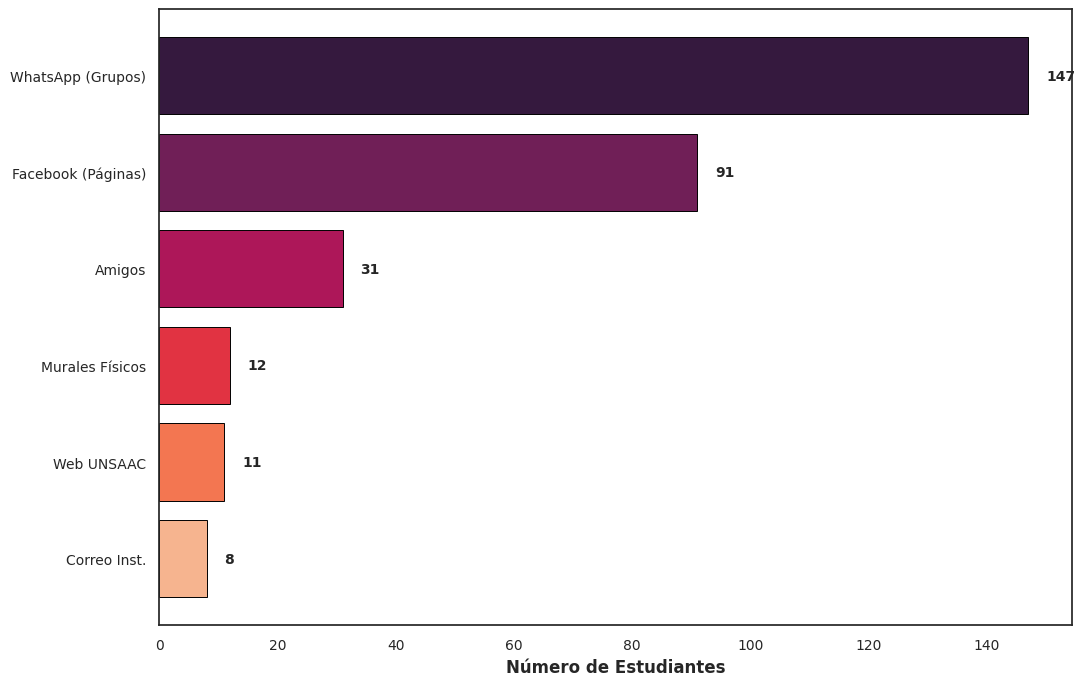
\includegraphics[width=0.88\linewidth,height=8cm,keepaspectratio]{imagenes/encuesta_03.png}\par
\captionof{figure}{Canales principales utilizados por las personas encuestadas}\label{fig:enc3}
\vspace{0.3cm}
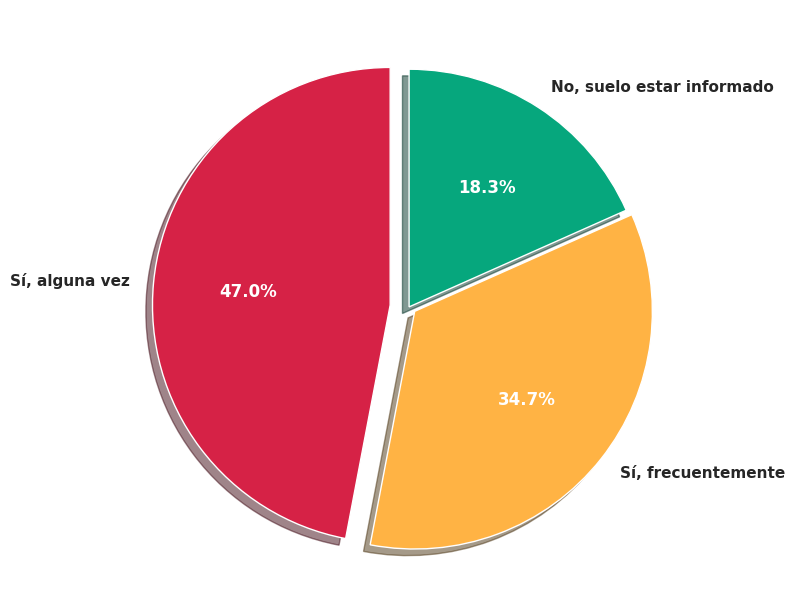
\includegraphics[width=0.88\linewidth,height=8cm,keepaspectratio]{imagenes/encuesta_04.png}\par
\captionof{figure}{Fechas importantes omitidas por falta de información oportuna}\label{fig:enc4}
\end{center}

\subsection{Alternativas para el servicio y la alimentación}
\textbf{A0. Mejora de canales existentes.} Ordenar fuentes, responsabilidades y una página central de avisos; difundir enlaces y QR mediante recursos disponibles. Es la comparación de menor equipamiento adicional.

\textbf{A1. Servicio interactivo con red eléctrica.} Añadir CMS, cliente público, tres terminales táctiles y respaldo dimensionado. Se evalúa si el acceso visible en espacios comunes aporta utilidad sobre A0.

\textbf{A2. Servicio interactivo con alimentación solar híbrida.} Integrar las funciones de A1 con generación FV, almacenamiento y gestión del circuito de cargas críticas. El conjunto de respaldo reemplaza los componentes equivalentes de A1; su costo se compara sobre la misma autonomía objetivo.

\cuadro{tab:alternativas}{Comparación preliminar de alternativas}{@{}P{3.0cm}Y Y Y@{}}{\textbf{Criterio}&\textbf{A0}&\textbf{A1}&\textbf{A2}}{
Información confiable & Depende de ordenar edición y fuentes & CMS y consulta trazable & Mismo beneficio informativo de A1\\*
Acceso presencial & Medios existentes y móvil & Tres puntos táctiles y QR & Igual cobertura física de A1\\
Complejidad & Menor integración & Cliente, red, soporte y energía & Añade FV, batería y estructura\\
Continuidad & Depende de medios existentes & Respaldo según carga & Respaldo central, FV y red de apoyo\\
Carga económica & Horas editoriales y canales & Equipos y servicio TI & A1 más inversión y operación solar\\
Decisión & Comprobar si resuelve la brecha & Demostrar valor de terminales & Justificar aporte y costo incremental\\
}
Se plantean dos decisiones: primero, si los terminales aportan valor frente a A0; después, si la generación aprovechada y las diferencias de desempeño justifican el incremento sobre A1.

Se formula A2 como alternativa integral del piloto y se conserva A1 como opción de ejecución por etapas. La decisión de inversión aplicará las reglas de comparación económica, capacidad operativa y aceptación técnica desarrolladas en el informe.

\subsection{Oferta y criterio de evaluación}
La oferta se compara por terminal completo, sistema soportado, orientación, cliente, energía, garantía y entrega en Cusco. El menor precio no determina cumplimiento. Las fichas oficiales respaldan características; las publicaciones comerciales respaldan sólo los importes y condiciones que explicitan.

Un tótem incluye pantalla, táctil, cómputo, carcasa y base. No se compara su precio con el de una pizarra horizontal o monitor suelto. Se solicitará una oferta homogénea para tres unidades, instalación y prueba, con impuestos, licencias y exclusiones explícitos.

\subsection{Comparación de terminales interactivos completos}
La unidad de comparación es el tótem vertical de piso con pantalla, superficie táctil, cómputo integrado, carcasa y base. Para la consulta interior se propone un mínimo de 55 pulgadas, resolución 4K, diez contactos táctiles y 400 cd/m\textsuperscript{2}; se prefieren 450 a 500 cd/m\textsuperscript{2} cuando la iluminación lo requiera. El ensayo en cada ubicación comprobará lectura, reflejos, altura y circulación.

El cuadro \ref{tab:fichas-totems} reúne cuatro ofertas publicadas en Perú y consultadas el 30 de octubre de 2026. Cada columna registra sólo lo que publica el vendedor, con su imagen referencial, precio, condición tributaria y los enlaces del producto y de la imagen. \emph{No publicado} indica un dato que la oferta deberá acreditar.

\begin{table}[p]\formatofichas
\caption{Tótems interactivos de 55 pulgadas analizados como opción}\label{tab:fichas-totems}
\begin{tabularx}{\linewidth}{@{}>{\raggedright\arraybackslash}p{2.15cm}YYYY@{}}
\toprule
\textbf{Característica} & \textbf{Prodimer TIPI7-55} & \textbf{First View FVD-D550M} & \textbf{Touch Data ADV5531, opción Pro} & \textbf{Visionsystems 55, Core i5}\\\midrule
\textbf{Imagen referencial} & \imgficha{imagenes/mercado_totem_prodimer.jpg}{3.0cm} & \imgficha{imagenes/mercado_totem_firstview.jpg}{3.0cm} & \imgficha{imagenes/mercado_totem_touchdata.jpg}{3.0cm} & \imgficha{imagenes/mercado_totem_visionsystems.jpg}{3.0cm}\\
\textbf{Proveedor} & Corporación Prodimer Perú S.A.C. & Perú Data Consult E.I.R.L., RUC 20486468913 & Touch Data Solutions & Visionsystems Perú, RUC 20511030332\\
\textbf{Procesador} & Core i7 de 13.\textsuperscript{a} generación; SKU no publicado & Core i7 de 13.\textsuperscript{a} generación; SKU no publicado & 13.\textsuperscript{a} generación; otras opciones: 8.\textsuperscript{a}, 6.\textsuperscript{a} y Android & Core i5; generación no publicada\\
\textbf{Memoria y SSD} & 16 GB; 256 GB & 16 GB DDR4; 256 o 512 GB & No publicados & No publicados\\
\textbf{Sistema} & Windows 11 Original; edición no publicada & Windows 11 Pro licenciado de fábrica & Windows con licencia; edición no publicada & Windows o Android; licencia no publicada\\
\textbf{Pantalla} & 3\,840 $\times$ 2\,160; 400 a 450 cd/m\textsuperscript{2} & LED 3\,840 $\times$ 2\,160; 450 cd/m\textsuperscript{2} & 4K vertical; brillo no publicado & 4K vertical; brillo no publicado\\
\textbf{Táctil} & Infrarrojo, 20 puntos & 20 puntos; la página indica infrarrojo y capacitivo & Infrarrojo, 10 puntos & Infrarrojo, 10 puntos\\
\textbf{Red, puertos y audio} & Wi-Fi 6, BT 5.4, RJ45, HDMI, VGA y USB 3.0 & Ethernet Gigabit, Wi-Fi 6, BT, HDMI, USB 3.0 y USB-C; parlantes de 8 W & No publicados & No publicados\\
\textbf{Energía y medidas} & 95 W sin condición de medición; medidas no publicadas & 100 a 240 V CA; 1\,900 $\times$ 850 $\times$ 100 mm; 85 kg brutos & No publicados & No publicados\\
\textbf{Garantía y alcance} & No indicada en el producto; política general de 36 meses & 3 años con el fabricante; producto a pedido & 1 año; incluye el software Touch Data Sign & 12 meses; entrega, instalación y software aparte\\
\textbf{Precio publicado} & S/~9\,499,99 por transferencia o S/~9\,974,99 con tarjeta; IGV no indicado & S/~10\,299,00; antes S/~11\,099,00; IGV no indicado & S/~7\,556,00 a S/~10\,794,00 + IGV según opción & S/~9\,999,00 con impuestos; 4 unidades disponibles\\
\textbf{Cota unitaria con IGV} & S/~11\,209,99 si fuera neto & S/~12\,152,82 si fuera neto & S/~12\,736,92 en el extremo superior & S/~9\,999,00 sin instalación ni software\\
\textbf{Enlace del producto} & \enlace{https://prodimerperu.com/producto/totem-interactivo-55-prodimer-peru/} & \enlace{https://www.perudataconsult.net/products/totem-interactivo-aio-electronics-55-touch-core-i7-13va-16gb-ddr4-ssd-256gb-w11pro-1-ano-fvd-d550m} & \enlace{https://touchdata.pe/producto/totem-vertical-touch-55/} & \enlace{https://visionsystemsperu.com/producto/totems-pantallas-publicitarias-leds-interactivos-touchs-screen-55-windows-android/}\\
\bottomrule
\end{tabularx}
\fuentefichas{Páginas de producto consultadas el 30 de octubre de 2026 \cite{prodimer,firstview,touchdata,visionsystems}. La cota con IGV aplica 18\% cuando la página no declara el tributo \cite{igv}. Fuente de las imágenes, de izquierda a derecha: \url{https://prodimerperu.com/wp-content/uploads/2026/06/TOTEM-PRODIMER-55-2.jpg}; \url{https://www.perudataconsult.net/cdn/shop/files/totem-1_9079a4dd-b94a-46e5-a063-dfc98ec8256e.jpg?v=1758993488}; \url{https://touchdata.pe/wp-content/uploads/2017/05/totem55webvj.jpg}; \url{https://visionsystemsperu.com/wp-content/uploads/2026/01/foto3.jpg}. Las imágenes son referenciales, se reproducen con fines académicos y su procedencia se registra en \texttt{procedencia\_imagenes.json}.}
\end{table}

\textbf{Opción elegida para valorizar ET-01: TIPI7-55}, porque publica la configuración Windows completa de menor precio con CPU admitida, brillo y táctil acreditados. Su política general de 36 meses de garantía rige sólo para bienes de fabricación propia, por lo que la oferta deberá declarar la garantía del tótem. Con la reserva tributaria y la reserva de licencia del presupuesto, la cota por terminal es S/~11\,559,99. First View documenta mejor licencia, garantía, medidas y masa, aunque su página alterna los códigos FVD-D550M y FVD-DS550M; con IGV incluido queda bajo esa cota y, si su precio fuera neto, la supera en S/~592,83 por unidad. Touch Data publica un rango con IGV aparte e incluye su propio CMS, no requerido en el escenario base. La oferta de Visionsystems no acredita brillo, memoria ni almacenamiento y excluye instalación y software. La contingencia cubre el peor caso de las alternativas comparadas; la selección se hará con ofertas homogéneas. La oferta final precisará procesador, edición y licencia del sistema, jornada admitida, potencia máxima del conjunto, base, anclajes y garantía.

La ruta GCS ADV-5542 de la versión anterior se retira de la comparación: su publicación en Sodimac figura sin existencias y sin precio \cite{gcstnt}. Hikvision DS-D6055UT-D/S se conserva como referencia documental de la ruta Android: Android 13, 4 GB/32 GB eMMC, 500 cd/m\textsuperscript{2}, 108 W típicos y 155 W máximos; no se encontró precio publicado en Perú \cite{hikvision}. La política de envío de Prodimer a provincias contempla agencia y flete en destino; se costearán transporte, descarga, instalación y atención en Cusco \cite{prodimer}.

\subsection{Matriz de cumplimiento y condición de suministro}
\textbf{C} indica acreditación documental en la ficha o publicación identificada; \textbf{P}, confirmación pendiente en la configuración ofertada o en su ensayo. La recepción comprobará el equipo entregado y el servicio integrado.

\cuadro{tab:mercado-cumplimiento}{Cumplimiento documental de los mínimos propuestos}{@{}Y P{1.95cm}P{1.95cm}P{1.95cm}P{1.95cm}@{}}{\textbf{Condición}&\textbf{Prodimer}&\textbf{First View}&\textbf{Touch Data}&\textbf{Vision\-systems}}{
55 pulgadas y estructura vertical de piso & C & C & C & C\\*
Pantalla 4K & C & C & C & C\\
Brillo de al menos 400 cd/m\textsuperscript{2} para interior & C & C: 450 & P & P\\
Diez contactos táctiles como mínimo & C: 20 & C: 20 & C: 10 & C: 10\\
CPU admitida por Windows 11; RAM y SSD declarados & C & C & P: RAM y SSD & P: generación, RAM y SSD\\
Sistema y licencia aptos para el cliente elegido & P & C: 11 Pro & P & P\\
Potencia máxima del terminal completo & P & P & P & P\\
Garantía del conjunto y atención en Cusco & P & P: 3 años & P: 1 año & P: 12 meses\\
Tratamiento tributario explícito & P & P & C: + IGV & C: incluido\\
Tres unidades, transporte e instalación en Cusco & P & P & P & P\\
}

La configuración Windows requerirá \textbf{Windows 11 Pro o una edición equivalente con licencia acreditada y funciones de bloqueo compatibles con el cliente}. Se incorpora una \textbf{reserva propia de S/ 350 por terminal, S/ 1\,050 en total}, para cerrar la edición y el derecho de uso cuando no estén incluidos en la oferta. Esta provisión se conciliará con el suministro para evitar duplicidades.

La mantenibilidad se evaluará mediante actualizaciones documentadas para un \textbf{horizonte objetivo de cinco años}, disponibilidad de controladores y repuestos, acceso técnico y una ruta de renovación del cliente. Windows 10 llegó al fin de soporte el 14 de octubre de 2025, sin asistencia técnica ni actualizaciones de seguridad posteriores \cite{win10fin}; no se aceptarán terminales con ese sistema. La lista de procesadores Intel admitidos por Windows 11 comienza en la 8.\textsuperscript{a} generación Core \cite{win11cpu}: la opción de 6.\textsuperscript{a} generación queda excluida y la de 8.\textsuperscript{a} requerirá soporte acreditado para el horizonte. Se exigirán exportación de contenidos y datos, separación entre administración y consulta pública y gestión de destinos por terminal. El horizonte constituye un criterio de planificación; el plazo contractual de garantía se establecerá por componente. La capacidad de CPU, RAM y almacenamiento se aceptará por el rendimiento del servicio, sin exigir la gama máxima.

\subsection{Fuentes de precio y catálogos electrónicos}
Los importes de este estudio son precios publicados por vendedores identificados. Sirven para la indagación de mercado de la formulación; no constituyen ofertas ni sustituyen las cotizaciones que solicite la entidad. Antes de convocar, el órgano encargado de las contrataciones verificará si los bienes figuran en los Catálogos Electrónicos de Acuerdos Marco, cuyo uso es obligatorio para los bienes catalogados, salvo las excepciones previstas \cite{contrataciones}.

El Buscador de Fichas de Producto de PERÚ COMPRAS informaba, con datos actualizados al 29 de octubre de 2026, 14 acuerdos marco de bienes vigentes y 26 catálogos. Son pertinentes EXT-CE-2024-2 Equipos multimedia y accesorios, EXT-CE-2022-5 Computadoras de escritorio, computadoras portátiles y escáneres, EXT-CE-2024-14 Luminarias, materiales eléctricos y cables eléctricos y EXT-CE-2024-1 Baterías, pilas y accesorios \cite{perucompras}. La verificación se hará por ficha-producto: el nombre de un catálogo no acredita que incluya un tótem de 55 pulgadas, un módulo FV, un inversor híbrido o el material eléctrico especificado.

La indagación comparará al menos dos ofertas homogéneas por componente. Cada una identificará proveedor y RUC, modelo exacto, moneda, impuestos, vigencia, plazo y lugar de entrega, garantía y exclusiones, con la fecha de consulta. Cuando la página comercial y la ficha del fabricante difieran, prevalecerá la ficha y la oferta deberá aclarar la diferencia.

\subsection{Alternativas de gestión de contenidos y costo del software}
Las tres rutas siguientes se evaluarán con las mismas funciones: permisos por grupo, preparación y revisión de avisos, programación y vencimiento, destinos, interacción táctil, consulta local y supervisión \cite{xibousers,xibotouch,xibodisplays}. La aprobación editorial deberá demostrarse con las cuentas y permisos configurados.

\cuadro{tab:mercado-cms}{Comparación de modalidades de CMS y reproductor}{@{}P{3.1cm}Y P{4.0cm}@{}}{\textbf{Modalidad}&\textbf{Operación y responsabilidad}&\textbf{Licencia o plan publicado}}{
CMS autoalojado y reproductor Windows & Administración del servidor, seguridad, copias, actualización del CMS y clientes a cargo del operador. Permite separar la plataforma de contenidos del terminal. & Núcleo y reproductor Windows abiertos bajo AGPLv3 o posterior, sin cargo por esas licencias \cite{xibolic}.\\*
CMS autoalojado y reproductor Android & Conserva las obligaciones del servidor; requiere instalación y prueba del reproductor en el SoC concreto. & USD 28 por reproductor perpetuo; tres: USD 84. Revisiones menores de la versión incluidas; actualización mayor según condiciones del fabricante \cite{xibolic}.\\
Xibo Cloud, plan Professional & Alojamiento del CMS, reproductor y soporte según el plan; el operador local conserva contenidos, equipos, conectividad y atención presencial. & USD 4,90 por pantalla-mes; tres: USD 14,70/mes y USD 176,40/año equivalentes \cite{xibolic}.\\
}

La base de software del presupuesto comprende \textbf{S/ 6\,000 para configuración y adaptación del CMS}, \textbf{S/ 3\,000 para interfaz y contenidos} y \textbf{S/ 720/año para alojamiento autoalojado}. Son estimaciones propias de planificación. La ausencia de cargo de licencia del software abierto mantiene las necesidades de configuración, operación y soporte. Al elegir un plan alojado se reemplazará la partida equivalente de alojamiento y se conciliará la licencia del reproductor. Los importes en USD se conservan en su moneda de publicación; facturación, conversión e impuestos se cerrarán al contratar.

\subsection{Prueba del cliente y criterio de selección tecnológica}
Xibo descarga medios, diseños y metadatos a una biblioteca local para reproducción sin conexión \cite{xibostorage}. El ensayo comprobará consulta, vencimiento, desconexión, reinicio sin red y actualización íntegra al reconectar. Una página externa integrada requerirá definir qué información se conserva localmente y cómo se valida su vigencia.

La ruta web o PWA deberá resolver ese mismo comportamiento. Las experiencias de kiosco de Edge utilizan InPrivate \cite{edge}; la continuidad tras reinicio exige probar la persistencia de la configuración elegida y, cuando corresponda, emplear un reproductor con biblioteca persistente o un paquete local controlado \cite{pwa,xibostorage}.

La pantalla 4K se distingue de la resolución con que se dibuja la interfaz. La documentación de Xibo para Android describe interfaz, imágenes y contenido web en 1080p escalados al panel 4K, con video nativo 4K \cite{xiboresolution}. La decisión valorará legibilidad y respuesta en el tótem real, sin prometer una interfaz nativa 4K por la resolución de la pantalla.



\clearpage
\section{Características técnicas del sistema}
\subsection{Alcance funcional y arquitectura}
El producto es un \textbf{servicio de información institucional}, compuesto por gestión editorial, consulta pública, distribución y continuidad. El piloto comprende tres terminales interiores de 55 pulgadas, red local de siete enlaces, videovigilancia de los terminales, CMS y cliente, contenido inicial, respaldo, subsistema FV, instalación, pruebas, capacitación y documentación. No incluye ampliar a toda la universidad, remodelación general, gestión de trámites con datos personales ni reemplazo de sistemas académicos.

La plataforma utilizará una administración central y clientes identificados por terminal y grupo. Se separarán publicación, consulta y supervisión mediante interfaces documentadas, con una base de datos y repositorio de medios respaldados. Esta arquitectura modular permite ampliar destinos y sustituir clientes sin rediseñar la gestión editorial.

\begin{center}
\begin{tikzpicture}[node distance=6mm,>=Latex,every node/.style={font=\small,align=center},box/.style={draw,rounded corners=2pt,text width=12.7cm,inner sep=6pt}]
\node[box] (f) {Fuentes autorizadas y emisores de la escuela\\Aviso, vínculo oficial, responsable e inicio/vencimiento};
\node[box,below=of f] (c) {CMS: borrador, revisión, aprobación y programación\\Cuentas individuales, permisos y registro de cambios};
\node[box,below=of c] (d) {Distribución de paquetes por versión y terminal\\Medios, vigencia, destino y confirmación de recepción};
\node[box,below=of d] (t) {Tres clientes públicos en modo kiosco\\Consulta táctil, QR, copia local y retorno al inicio};
\node[box,below=of t] (m) {Supervisión y continuidad\\Última comunicación, versión, incidencias y recuperación};
\draw[->](f)--(c);\draw[->](c)--(d);\draw[->](d)--(t);\draw[<->](t)--(m);
\end{tikzpicture}
\captionof{figure}{Arquitectura funcional del servicio de información}
\label{fig:arquitectura}
\end{center}

\subsection{Proceso editorial y modelo de información}
Cada aviso tendrá identificador, título, categoría, emisor, fuente oficial, texto o medio, inicio, vencimiento, destino y versión. La operación distinguirá contenido en borrador, en revisión, aprobado, publicado, vencido y retirado. El editor preparará; el revisor comprobará fuente y vigencia; el sistema publicará sólo la versión autorizada.

La primera operación utilizará carga validada de fuentes oficiales. Cada integración automática requerirá titular, autorización, formato, frecuencia, autenticación, campos y manejo de errores. La versión y la fuente del aviso permitirán rastrear su publicación y retirada.

El cuadro \ref{tab:fuentes_contenido} identifica de dónde procede cada tipo de información, quién la entrega y cómo ingresa al servicio. Los emisores son propuestos y la dirección de escuela los designará antes de la puesta en servicio.

\cuadro{tab:fuentes_contenido}{Origen, emisor y forma de ingreso de la información publicada}{@{}P{2.7cm}P{3.6cm}Y P{2.0cm}@{}}{\textbf{Información}&\textbf{Fuente oficial y emisor propuesto}&\textbf{Forma de ingreso y control}&\textbf{Vigencia}}{
Trámites y calendario & Dirección de escuela y secretaría académica; calendario y resoluciones de la universidad & El editor transcribe el aviso y enlaza el documento oficial; revisión antes de publicar & Hasta la fecha límite\\*
Becas y créditos & Unidades de bienestar y oficinas de becas; convocatorias oficiales externas & Aviso con enlace a la convocatoria y fecha de cierre; dato exigido por el art. 11.4 & Hasta el cierre\\
Eventos y capacitación & Escuela, centro federado y unidades organizadoras & Formulario interno del emisor y aprobación del revisor & Hasta el evento\\
Oportunidades profesionales & Convenios, prácticas y bolsa de trabajo de la universidad & Sólo ofertas con entidad identificada y enlace verificable & Hasta la postulación\\
Investigación y proyectos & Docentes responsables y grupos de investigación & Ficha autorizada por el titular; sin datos personales no consentidos & Semestral\\
Avisos urgentes & Dirección de escuela & Publicación prioritaria con doble verificación y retiro programado & Horas o días\\
}
El servicio no genera información propia ni reemplaza el documento oficial. Muestra un resumen verificable y el QR al documento de origen. Cuando una fuente se integre de forma automática, su formato y frecuencia se acordarán con el titular, conforme al requisito RF09.

\cuadro{tab:requisitos}{Requisitos funcionales y evidencia de aceptación}{@{}P{1.0cm}P{3.1cm}Y@{}}{\textbf{ID}&\textbf{Función}&\textbf{Criterio verificable}}{
RF01 & Consulta pública & Buscar categorías y abrir detalle; fuente y vigencia visibles, sin cuenta del estudiante\\*
RF02 & Edición y aprobación & Crear, revisar y programar; impedir publicación sin campos y autorización requeridos\\
RF03 & Destinos & Publicar en una, varias o todas las terminales; confirmar versión aplicada\\
RF04 & Caducidad & Retirar o advertir avisos vencidos, incluso bajo la política local de contingencia\\
RF05 & Consulta QR & Abrir vínculo institucional desde móvil; no encerrar información sólo en el edificio\\
RF06 & Continuidad & Conservar paquete aprobado y recuperar consulta tras corte de red y reinicio\\
RF07 & Supervisión & Registrar última comunicación, versión y errores; generar y asignar incidencia\\
RF08 & Auditoría & Conservar autor, revisor, fecha y cambios; exportar registro autorizado\\
RF09 & Integración condicionada & Validar esquema y permisos antes de consumir fuentes automáticas\\
}
Se priorizan RF01 a RF08. Las funciones de colaboración difundirán proyectos y contactos autorizados. RF09 se incorporará después de acreditar acceso e interoperabilidad con la fuente institucional.

\subsection{Experiencia de consulta e interfaz}
La consulta se organiza por oportunidades, eventos, trámites, información académica y proyectos de colaboración. Cada detalle mostrará fuente, fecha y vigencia; un código QR permitirá continuar la lectura en móvil. El inicio recuperará una vista simple tras inactividad y evitará formularios con datos personales en la terminal pública.
\begin{center}
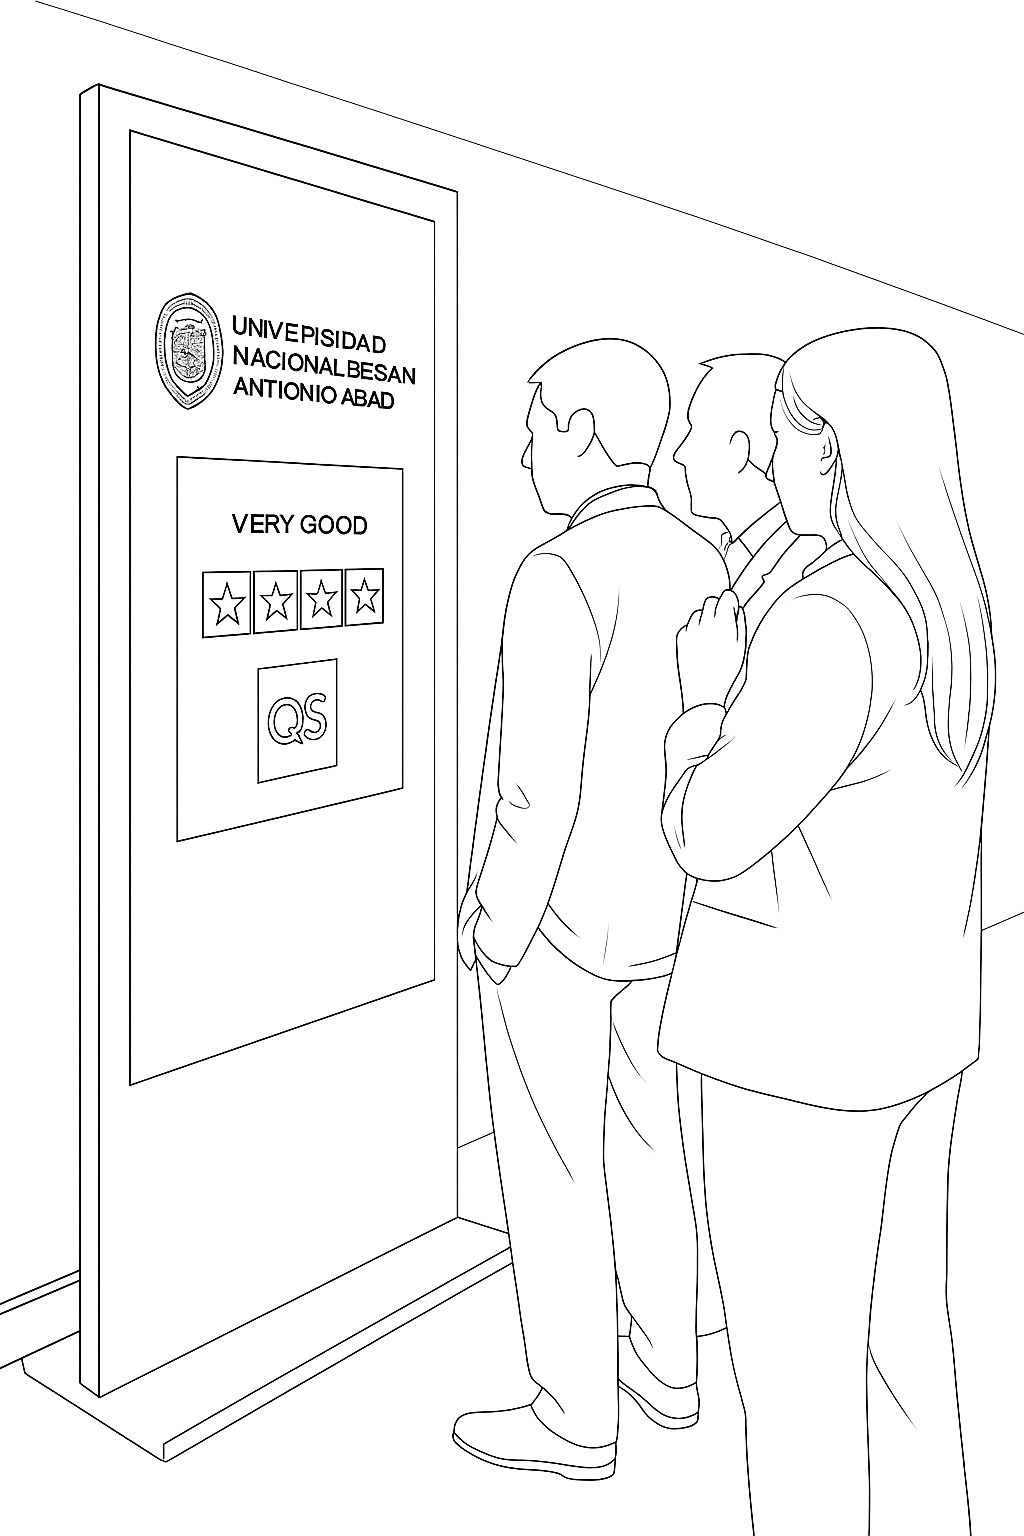
\includegraphics[width=0.47\linewidth,height=12cm,keepaspectratio]{imagenes/concepto_terminal.png}\hfill
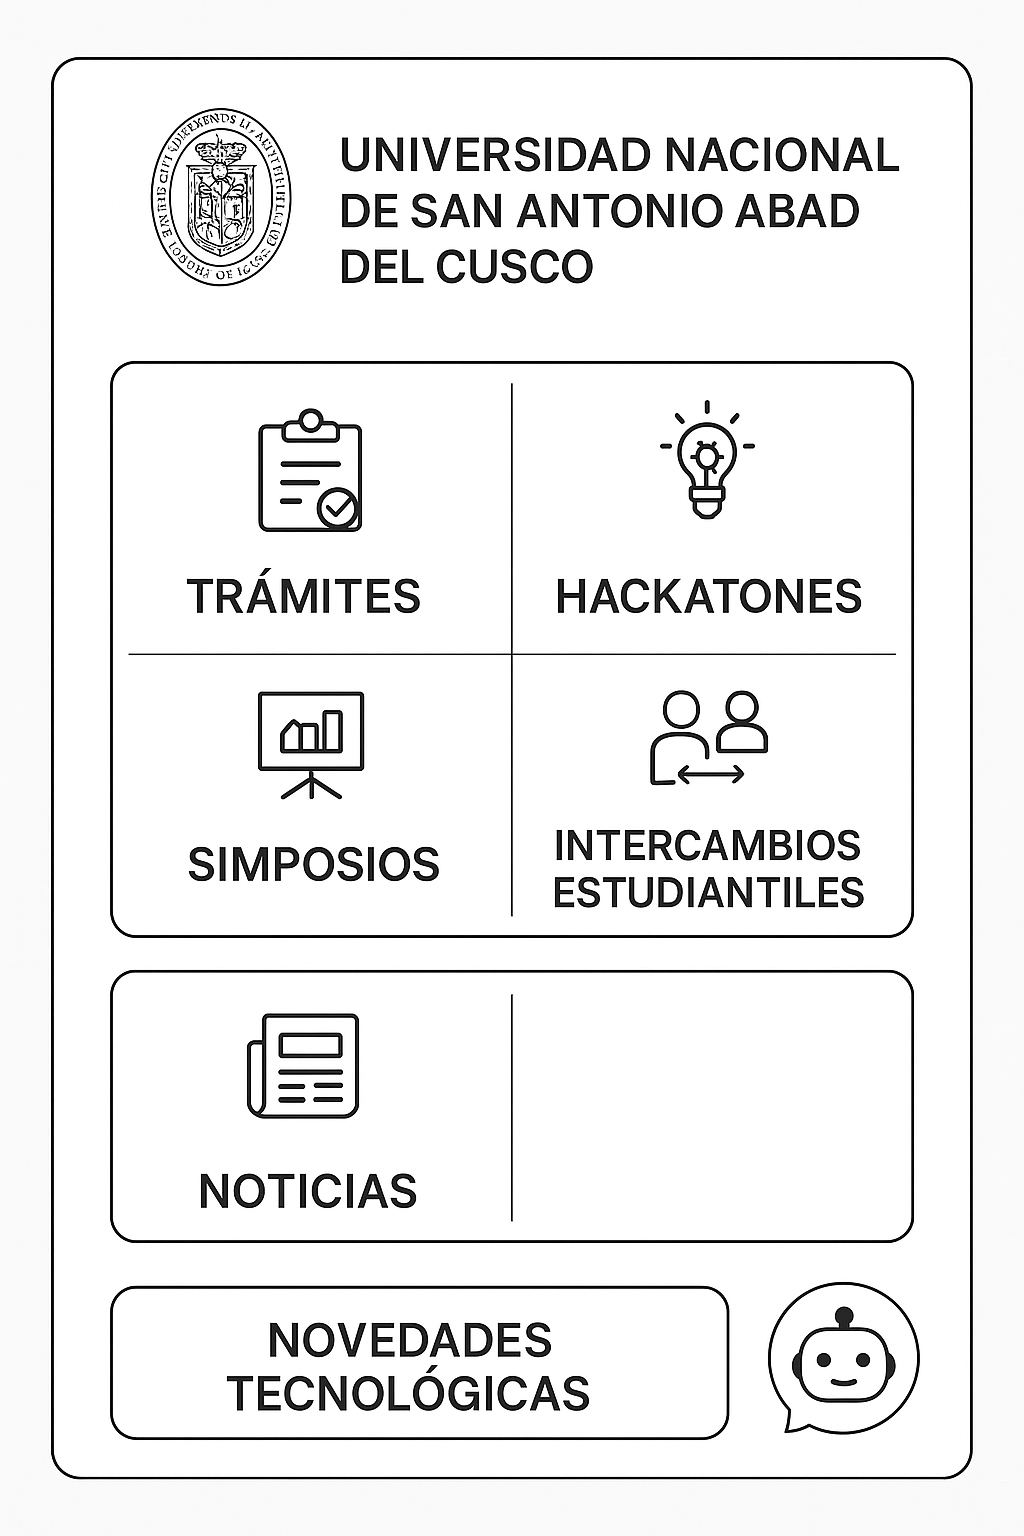
\includegraphics[width=0.47\linewidth,height=12cm,keepaspectratio]{imagenes/concepto_interfaz.png}\par
\captionof{figure}{Diseño conceptual del terminal y de la consulta por categorías}\label{fig:concepto}
\end{center}
Los bocetos orientan la organización visual. La versión funcional se adaptará a las categorías aprobadas, al reproductor y a las pruebas de legibilidad, navegación y accesibilidad.
\begin{center}
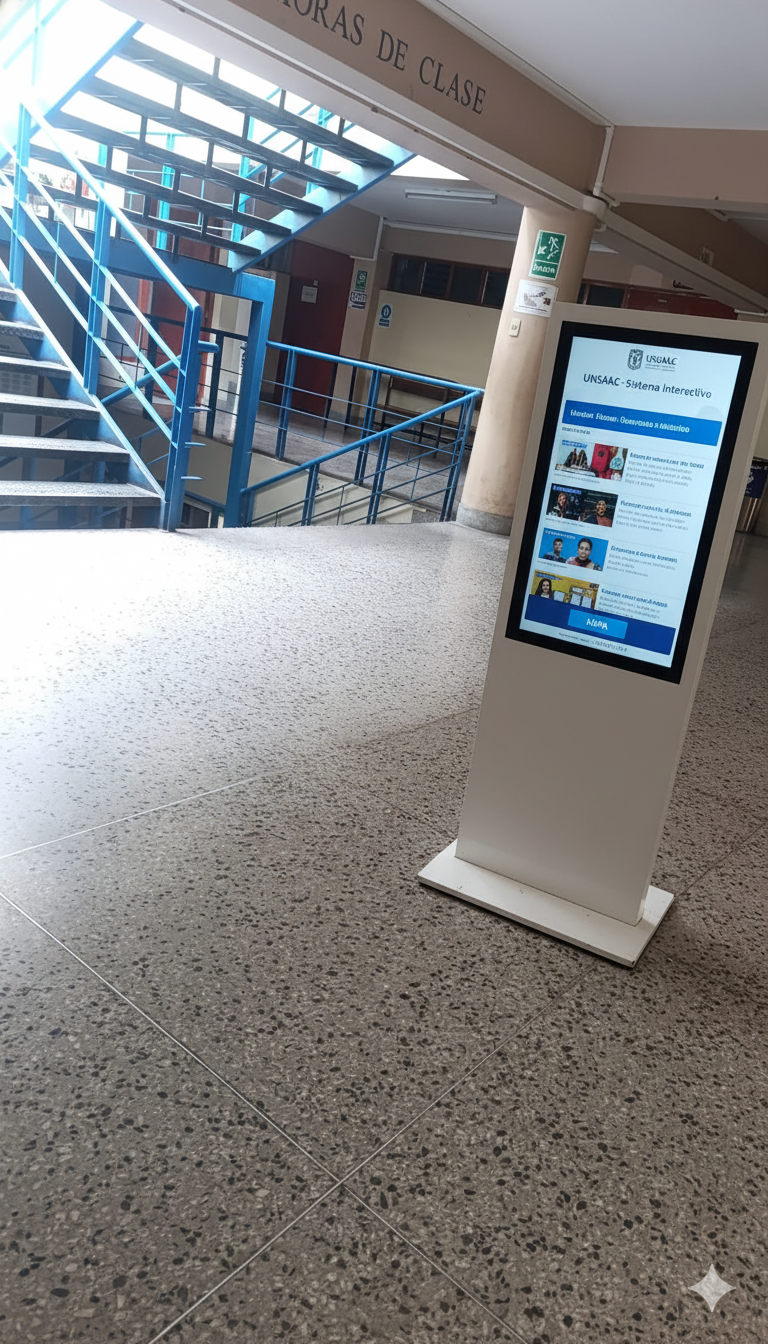
\includegraphics[height=14cm,keepaspectratio]{imagenes/visualizacion_ubicacion.png}\par
\captionof{figure}{Visualización conceptual del emplazamiento propuesto}\label{fig:visualizacion}
\end{center}
\subsection{Datos, interfaces y trazabilidad}
La gestión editorial mantendrá un modelo de información único para las terminales y la consulta móvil. La publicación separará el aviso de sus destinos, de modo que una corrección genere una nueva versión y se propague de forma controlada.

\cuadro{tab:datos}{Modelo lógico de información del servicio}{@{}P{2.5cm}Y Y@{}}{\textbf{Entidad}&\textbf{Datos esenciales}&\textbf{Relación y control}}{
Aviso y versión & Identificador, categoría, título, texto/medio, fuente, emisor y versión & Cada cambio conserva autor y fecha; publicación ligada a una versión\\*
Publicación & Aviso/versión, destino, inicio, vencimiento y aprobación & Un aviso puede publicarse en varios destinos y franjas\\
Terminal & Identificador, piso, cliente, versión aplicada y última comunicación & Destinos por terminal o grupo; estado técnico diferenciado de legibilidad\\
Usuario y permiso & Cuenta, rol, destinos autorizados y estado & Publicación y administración separadas de consulta pública\\
Incidencia & Síntoma, origen, prioridad, responsable y solución & Relacionada con terminal, versión o integración afectada\\
Medición energética & Fecha, intervalo, kWh, origen y calidad del dato & Serie exportable; distingue FV, red, cargas y estimación de batería\\
}
Se documentarán formato de exportación, retención y restauración. Los paquetes de contenido identificarán versión y manifiesto de medios. La recepción comprobará integridad antes de activar una actualización; el cliente conservará una versión funcional de recuperación.

\cuadro{tab:no_funcionales}{Condiciones no funcionales de diseño y prueba}{@{}P{2.6cm}Y@{}}{\textbf{Aspecto}&\textbf{Criterio de trabajo}}{
Respuesta de consulta & Detalle local en hasta 3 s para 95\% de intentos del ensayo; medir con el paquete y equipo previstos\\*
Capacidad inicial & 3 destinos físicos, 500 avisos de prueba y medios con tamaño y formato limitados por política\\
Publicación & Versión aprobada disponible en hasta 5 min en terminal conectada durante el ensayo\\
Disponibilidad & Objetivo inicial 98\% del horario de servicio, con interrupciones y mantenimiento registrados\\
Recuperación & RPO de hasta 24 h para contenido respaldado y RTO de hasta 8 h de atención; restauración ensayada\\
Seguridad y acceso & Administración autenticada, permisos por destino, tráfico protegido y salida del kiosco restringida\\
Mantenibilidad & Inventario, configuración versionada, registros exportables, actualización probada y ruta de sustitución del cliente\\
}
Los objetivos se medirán durante el piloto. La aceptación inicial utilizará los casos de prueba; el seguimiento verificará su continuidad en el horario real de operación.

\subsection{Requerimientos de software y selección de plataforma}
Se compararán dos rutas sobre los mismos casos de uso: \textbf{configurar un CMS de señalización existente} y \textbf{desarrollar un CMS con cliente específico}. La primera puede reducir trabajo inicial; la segunda permite adaptar flujos, pero aumenta responsabilidad de mantenimiento y pruebas.

Xibo ofrece funciones documentadas de usuarios, grupos, pantallas, programación y acciones táctiles \cite{xibousers,xibotouch,xibodisplays}. Permite evaluar un CMS configurable. La compatibilidad del reproductor, las licencias por plataforma y el alojamiento se comprobarán para el conjunto concreto; software abierto no significa implantación ni operación sin costo \cite{xibolic}.

Un cliente web o PWA es otra opción; sus funciones de almacenamiento deben diseñarse y comprobarse. Microsoft documenta que el modo de señalización de Edge utiliza InPrivate \cite{edge}. Por ello, no se garantiza persistencia de contenidos después de reiniciar sólo por utilizar un navegador. El ensayo exigirá reinicio sin red; si la configuración no conserva los paquetes, se requerirá un reproductor con almacenamiento persistente o un paquete local controlado.

\cuadro{tab:software}{Comparación de rutas de software}{@{}P{3.0cm}Y Y@{}}{\textbf{Criterio}&\textbf{CMS configurable}&\textbf{CMS y cliente propios}}{
Publicación y destinos & Configurar funciones existentes y demostrar permisos & Implementar y probar flujo completo\\*
Interacción & Validar acciones táctiles en reproductor real & Diseñar interfaz y navegación específicas\\
Sin conexión & Probar medios descargados y caducidad; URL externa no queda copiada automáticamente & Diseñar caché persistente, versiones y recuperación\\
Costo & Configuración, licencias aplicables, alojamiento y soporte & Análisis, desarrollo, pruebas, despliegue y mantenimiento\\
Decisión & Preferible si satisface los casos sin extensiones costosas & Justificable si hay brechas funcionales relevantes y capacidad de soporte\\
}
Se recomienda demostrar primero la ruta configurable. El presupuesto reserva trabajo de adaptación; si los ensayos exigen desarrollo mayor, se revisará esfuerzo y alternativa antes de comprometer alcance.

\subsection{Hardware y ubicación}
\cuadro{tab:hardware}{Especificaciones funcionales del piloto}{@{}P{3.0cm}Y P{2.5cm}@{}}{\textbf{Componente}&\textbf{Características propuestas}&\textbf{Cantidad}}{
Terminal completo & Interior, piso anclable, aproximadamente 55 pulgadas, vertical 4K, mínimo 10 contactos táctiles y acceso técnico protegido & 3 unidades\\*
Visualización & Panel 4K vertical; brillo de referencia mínimo 400 nits en interior y legibilidad verificada; 450 a 500 nits preferibles con reflejos & En cada terminal\\
Cómputo y sistema & Cliente Windows con 16 GB/256 GB como referencia, o Android con recursos demostrados; sistema licenciado y soporte documentado & Integrado o incluido\\
Red & Cableado Cat 6 de cobre, switch administrable y gabinete; direccionamiento y segmentación acordados; Wi-Fi sólo si se valida & 7 enlaces y 1 gabinete\\
Videovigilancia & Una cámara IP por terminal y grabador local con 30 días de conservación & 3 cámaras y 1 NVR\\
CMS y respaldo & Alojamiento, copias separadas, cuentas de gestión y recuperación & 1 servicio central\\
Alimentación & Circuito de cargas críticas, protecciones y puesta a tierra según diseño; FV y batería compatibles & 1 sistema integrado\\
}
El cuadro resume la función de cada componente. Los mínimos exigibles, sin marca ni modelo, se desarrollan como especificaciones ET-01 a ET-10 en la sección \ref{sec:especificaciones}. La opción de mercado usada para valorizar cada uno se elige en la sección \ref{sec:seleccion}. El suministro identificará CPU exacta, edición y licencia del sistema, potencia máxima, garantía e instalación.

Se adopta una cota de diseño de 200 W por terminal completo. Las ofertas comparadas publican 95 W sin condición de medición, y la ficha de una ruta Android de 55 pulgadas declara 108 W típicos y 155 W máximos \cite{prodimer,hikvision}. Una oferta con mayor consumo obligará a recalcular el sistema energético. El horario del servicio es de 12 horas al día. La aprobación de un cliente Android incluirá instalación del reproductor, persistencia, legibilidad y soporte de actualizaciones.

La distribución por piso y la propuesta de interfaz se desarrollan en las secciones siguientes. El diseño de instalación incluirá circulación, alcance de uso, anclajes y condiciones de mantenimiento.

\subsection{Emplazamiento y distribución del piloto}
Se plantea un terminal por piso. El levantamiento contrastará las posiciones de los planos con tránsito, visibilidad, reflejos, aproximación, circulación y acceso de mantenimiento. La definición final incorporará los recorridos de red y del circuito protegido.

\subsubsection{Primer piso}
\begin{center}
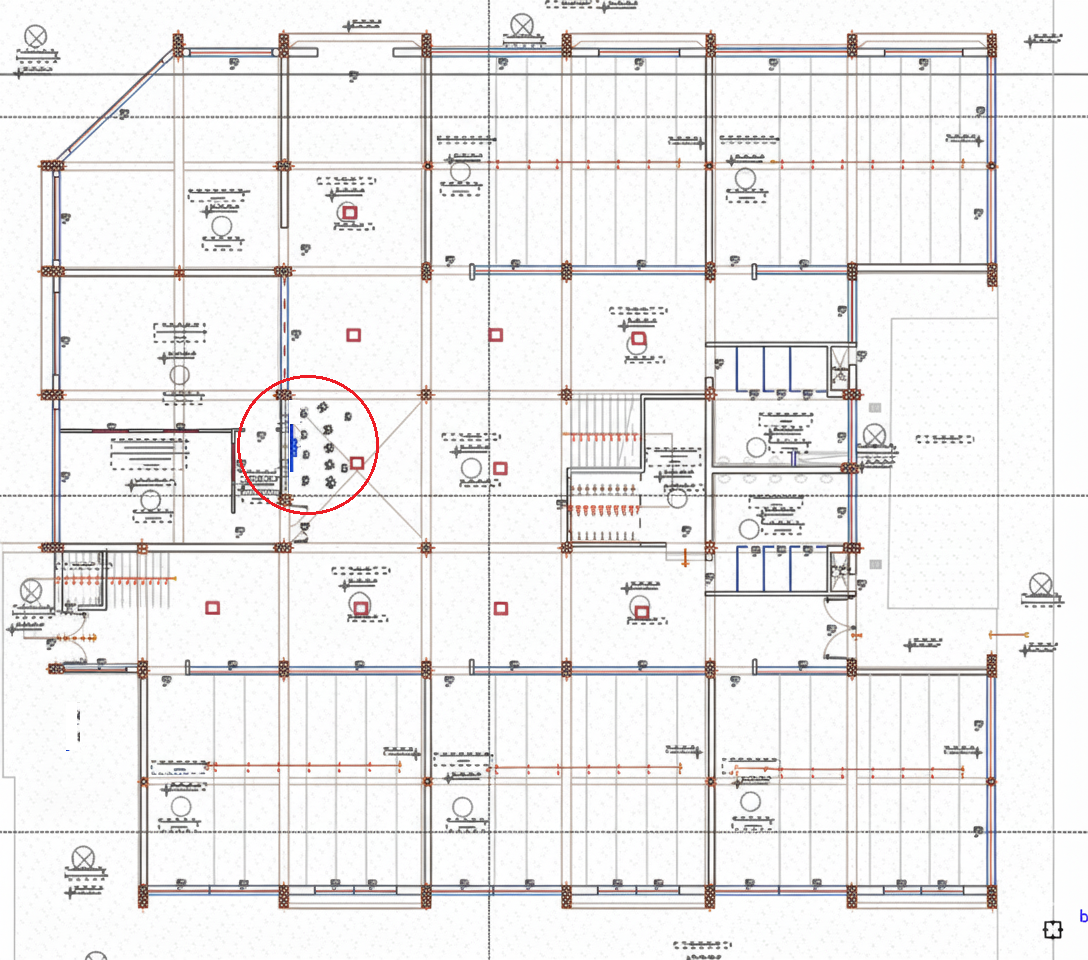
\includegraphics[width=\linewidth,height=12.2cm,keepaspectratio]{imagenes/planta_piso_1.png}\par
\vspace{0.15cm}
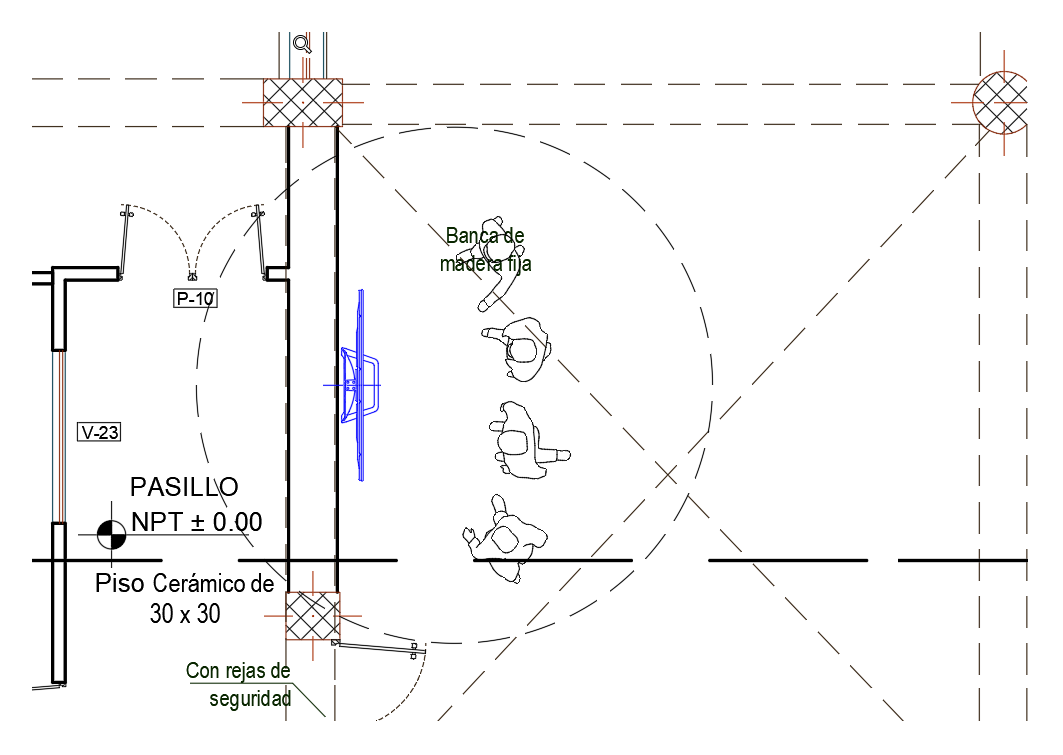
\includegraphics[width=\linewidth,height=5.0cm,keepaspectratio]{imagenes/detalle_piso_1.png}\par
\captionof{figure}{Planta y detalle de ubicación propuesta en el primer piso}\label{fig:piso1}
\end{center}
\clearpage
\subsubsection{Segundo piso}
\begin{center}
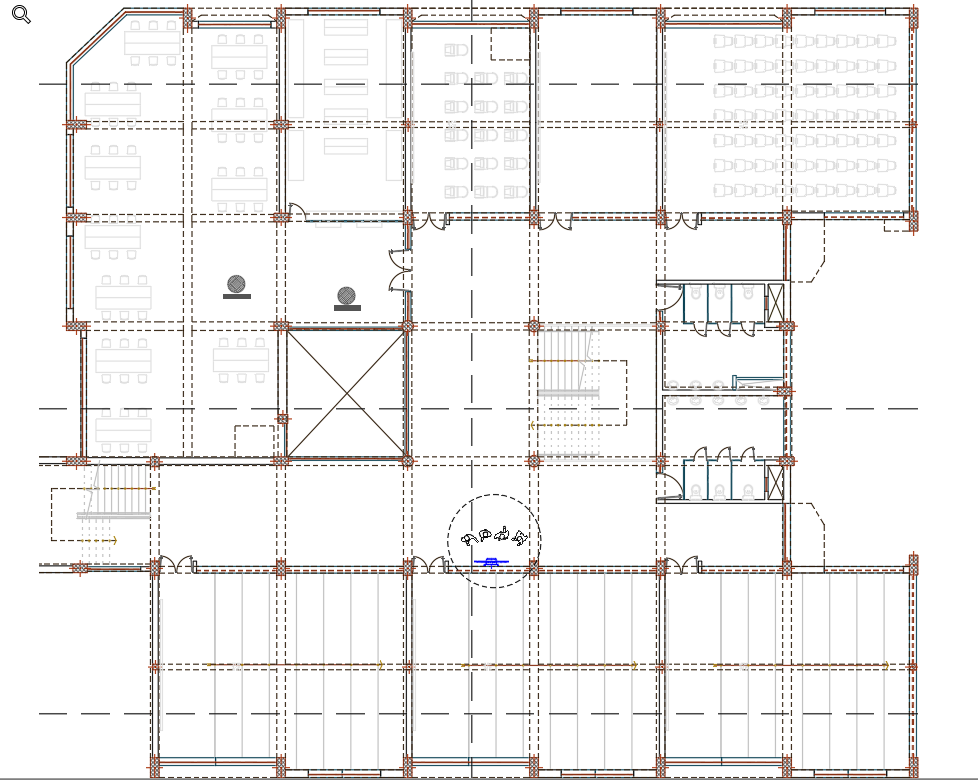
\includegraphics[width=\linewidth,height=13cm,keepaspectratio]{imagenes/planta_piso_2.png}\par
\vspace{0.25cm}
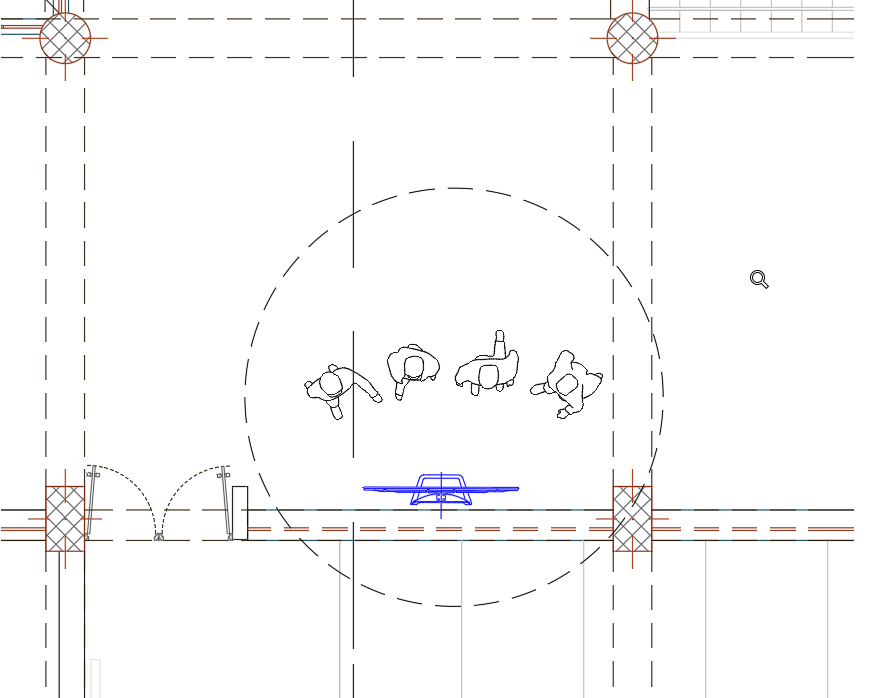
\includegraphics[width=\linewidth,height=5.5cm,keepaspectratio]{imagenes/detalle_piso_2.png}\par
\captionof{figure}{Planta y detalle de ubicación propuesta en el segundo piso}\label{fig:piso2}
\end{center}
\clearpage
\subsubsection{Tercer piso}
\begin{center}
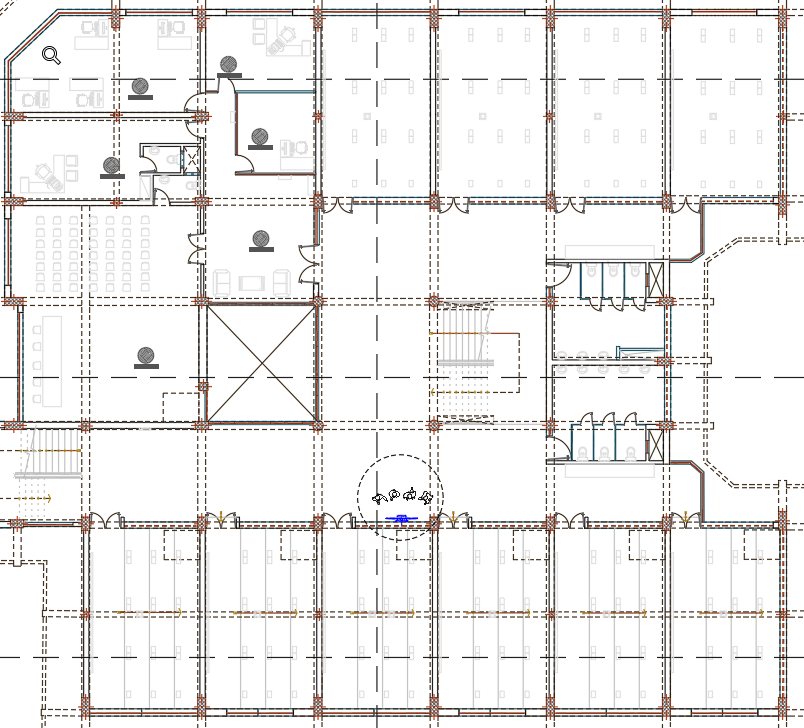
\includegraphics[width=\linewidth,height=13cm,keepaspectratio]{imagenes/planta_piso_3.png}\par
\vspace{0.25cm}
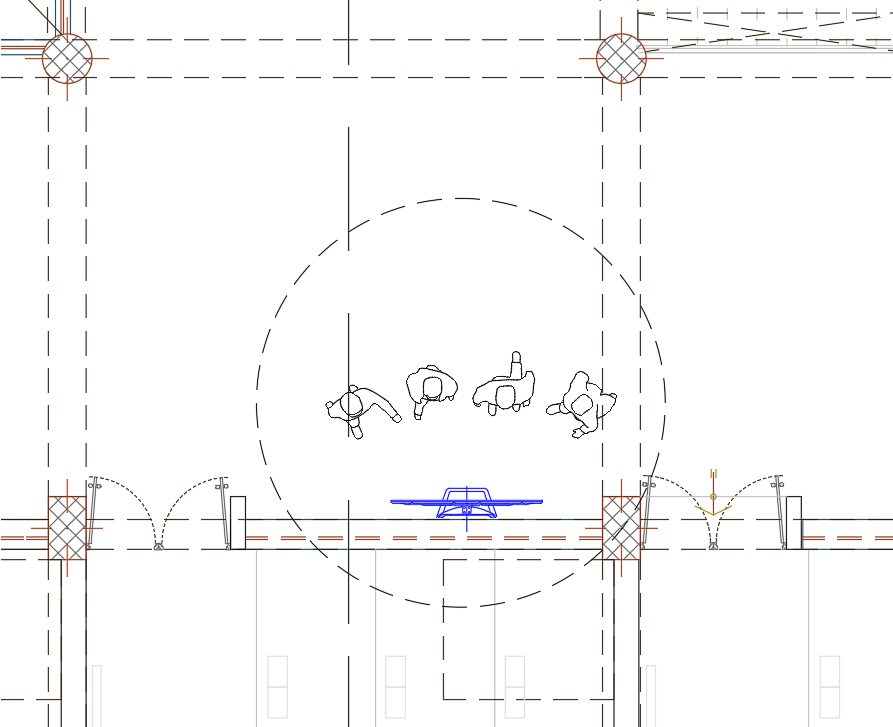
\includegraphics[width=\linewidth,height=5.5cm,keepaspectratio]{imagenes/detalle_piso_3.png}\par
\captionof{figure}{Planta y detalle de ubicación propuesta en el tercer piso}\label{fig:piso3}
\end{center}
\clearpage

\subsection{Seguridad, accesibilidad y continuidad}
\begin{itemize}
\item Cuentas individuales para administración; permisos por función y destino; consulta pública sin acceso al escritorio ni a la edición.
\item Conexión protegida, actualizaciones controladas, dominios autorizados y credenciales fuera de la interfaz pública.
\item Botones legibles, contraste, retorno al inicio por inactividad y alternativa mediante QR; altura y aproximación verificadas en la ubicación.
\item Audio desactivado por defecto o limitado según condiciones del espacio. No depender sólo de audio o color para comunicar información.
\item Copia diaria inicial de CMS, medios y configuración; ensayo de restauración. Objetivos de trabajo: pérdida de datos recuperables hasta 24 h y recuperación en 8 h de atención, por acordar con TI.
\item Durante desconexión, mostrar última sincronización y consultar sólo contenido local permitido por su vigencia. Las alertas urgentes no se presentarán como actuales sin confirmación.
\end{itemize}
La última comunicación del cliente no demuestra por sí sola que la pantalla esté encendida o sea legible. Se combinará supervisión técnica con comprobación visual y reporte de usuarios.

\subsection{Comparación tecnológica de módulos fotovoltaicos}
Se contrastan cuatro módulos publicados por un mismo distribuidor en Perú, AutoSolar, para homogeneizar IGV, existencias y despacho. La selección considera costo por Wp, corriente frente al límite de 16~A del seguidor MPPT, tensión del string en frío, área, masa y garantía, además de la potencia nominal. Cuando la página comercial y la ficha del fabricante difieren, prevalece la ficha. Una generación tecnológica más reciente puede mejorar el aprovechamiento del área, pero no demuestra por sí sola menor costo del servicio ni compatibilidad con el inversor. El cuadro \ref{tab:modulos_comparados} presenta las cuatro opciones con su imagen referencial, datos de ficha, precio y enlaces.

Jinko conserva el menor costo por Wp y se mantiene como referencia de valorización. Su Imp STC deja un margen de 5,3\% frente a los 16~A del seguidor, pero la corriente bifacial BNPI de 16,73~A lo supera: no se presupone ganancia posterior y se evaluará la limitación de corriente \cite{jinko}. AutoSolar declara además una garantía propia de un año en esa página; la garantía de 12 años corresponde al fabricante y su atención deberá acreditarse \cite{preciojinko}.

La página de Trina anuncia un módulo bifacial, mientras la ficha que enlaza corresponde al TSM-NE19R.70 de lámina posterior \cite{trinaprecio,trinaficha}. La oferta deberá identificar el modelo exacto. Si se confirma esa ficha, el conjunto pesa 28,2~kg menos y amplía el margen de corriente por S/~168,30 adicionales. LONGi Hi-MO X10 ofrece la mayor eficiencia y 15 años de garantía de producto, con S/~926,04 adicionales y el menor margen de corriente. El módulo LONGi de 505~W es la única opción con holgura amplia frente al seguidor; utiliza tecnología PERC, requiere siete unidades y eleva el costo en S/~2\,355,90 \cite{longi505ficha}.

\textbf{Opción elegida para valorizar ET-06: Jinko Tiger Neo de 615~W}, por menor costo por Wp entre las que cumplen tensión, área y garantía. Las cuatro tensiones del string en frío permanecen bajo los 550~V del inversor elegido y dentro de su rango MPPT de 40 a 530~V. Si la ingeniería concluye que la limitación de corriente del módulo de referencia es inaceptable, se confirmará el Trina de lámina posterior, se adoptará el módulo de 505~W o se cotizará un inversor con mayor corriente por seguidor; cualquiera de esas decisiones requerirá recalcular el conjunto. Las garantías de ficha no reemplazan las condiciones contractuales, exclusiones y atención local que debe acreditar el proveedor.

\begin{table}[p]\formatofichas
\caption{Paneles solares analizados como opción: características STC y precio unitario}\label{tab:modulos_comparados}
\begin{tabularx}{\linewidth}{@{}>{\raggedright\arraybackslash}p{2.15cm}YYYY@{}}
\toprule
\textbf{Característica} & \textbf{Jinko Tiger Neo 615~W} & \textbf{Trina Vertex N 625~W} & \textbf{LONGi Hi-MO X10 640~W} & \textbf{LONGi Hi-MO 5 505~W}\\\midrule
\textbf{Imagen referencial} & \imgficha{imagenes/mercado_fv_jinko615.jpg}{3.1cm} & \imgficha{imagenes/mercado_fv_trina625.jpg}{3.1cm} & \imgficha{imagenes/mercado_fv_longi640.jpg}{3.1cm} & \imgficha{imagenes/mercado_fv_longi505.jpg}{3.1cm}\\
\textbf{Modelo y tecnología} & JKM615N-66HL4M-BDV; TOPCon tipo N, bifacial, doble vidrio & TSM-NE19R.70 según la ficha: i-TOPCon con lámina posterior; la página dice bifacial & LR8-66HVD-640M; contacto posterior HPBC 2.0, bifacial, doble vidrio & LR5-66HPH-505M; PERC de media celda, vidrio simple; ficha de 2022\\
\textbf{Potencia y eficiencia} & 615 Wp; 22,77\% & 625 Wp; 23,1\% & 640 Wp; 23,7\% & 505 Wp; 21,3\%\\
\textbf{Vmp / Imp STC} & 40,60 V / 15,15 A & 41,6 V / 15,00 A & 40,78 V / 15,69 A & 38,53 V / 13,11 A\\
\textbf{Voc / Isc STC} & 48,88 V / 16,02 A & 49,8 V / 15,93 A & 49,52 V / 16,38 A & 45,70 V / 13,97 A\\
\textbf{Coeficiente de Voc} & $-0{,}25$\,\%/°C & $-0{,}24$\,\%/°C & $-0{,}20$\,\%/°C & $-0{,}265$\,\%/°C\\
\textbf{Medidas y masa} & 2\,382 $\times$ 1\,134 $\times$ 30 mm; 32,4 kg & 2\,382 $\times$ 1\,134 $\times$ 30 mm; 27,7 kg & 2\,382 $\times$ 1\,134 $\times$ 30 mm; 33,5 kg & 2\,093 $\times$ 1\,134 $\times$ 35 mm; 25,3 kg\\
\textbf{Garantía} & 12 y 30 años & 12 y 25 años & 15 y 30 años & 12 y 25 años\\
\textbf{Precio con IGV} & S/~405,35; S/~0,659 por Wp; sin IGV S/~343,52 & S/~433,40; S/~0,693 por Wp; sin IGV S/~367,29 & S/~559,69; S/~0,875 por Wp; sin IGV S/~474,31 & S/~684,00; S/~1,354 por Wp; sin IGV S/~579,66\\
\textbf{Conjunto para el balance} & 6 módulos; 3,69 kWp; S/~2\,432,10; 16,21 m$^2$; 194,4 kg & 6 módulos; 3,75 kWp; S/~2\,600,40; 16,21 m$^2$; 166,2 kg & 6 módulos; 3,84 kWp; S/~3\,358,14; 16,21 m$^2$; 201,0 kg & 7 módulos; 3,535 kWp; S/~4\,788,00; 16,61 m$^2$; 177,1 kg\\
\textbf{Margen de Imp a 16 A} & 5,3\%; la corriente BNPI de 16,73 A lo supera & 6,3\%; sin ganancia posterior si se confirma la ficha & 1,9\%; con 5\% de ganancia posterior, unos 16,47 A; la ficha tabula 16,57 A sobre base de 645 W & 18,1\%; módulo monofacial\\
\textbf{Voc del string a $-10$\,°C} & 318,94 V & 323,90 V & 317,92 V & 349,57 V\\
\textbf{Enlace del producto} & \enlace{https://autosolar.pe/paneles-solares-24v/panel-solar-jinko-tiger-neo-bifacial-615w-n-type} & \enlace{https://autosolar.pe/paneles-solares/panel-solar-bifacial-625w-trina-solar} & \enlace{https://autosolar.pe/paneles-solares-24v/panel-solar-bifacial-longi-lr8-66hvd-640m-hi-mo-640w} & \enlace{https://autosolar.pe/paneles-solares-24v/panel-solar-longi-lr5-66hph-himo5-505w}\\
\bottomrule
\end{tabularx}
\fuentefichas{Páginas de AutoSolar Perú y fichas de fabricante consultadas el 30 de octubre de 2026 \cite{preciojinko,jinko,trinaprecio,trinaficha,longiprecio2026,longificha2025,longi505precio,longi505ficha}. STC corresponde a condiciones normalizadas de ensayo; la garantía indica años de producto y de potencia lineal. El número de módulos es $N=\lceil 1{,}20(8{,}16)/(3P)\rceil$, con $P$ en kW, 4 HSP y factor 0,75; el margen de corriente es $(16-I_{mp})/16$. Fuente de las imágenes, de izquierda a derecha: \url{https://cdn.autosolar.pe/images/1002232/panel-solar-jinko-tiger-neo-bifacial-615w-n-type-684992fe19b4e.jpg}; \url{https://cdn.autosolar.pe/images/1002343/panel-solar-bifacial-625w-trina-solar-698dfb53e7a67.jpg}; \url{https://cdn.autosolar.pe/images/1006015/panel-solar-bifacial-longi-lr8-66hvd-640m-hi-mo-640w-69a9f09bd1a5f.jpg}; \url{https://cdn.autosolar.pe/images/1006012/panel-solar-longi-lr5-66hph-himo5-505w.jpg}. Las imágenes son referenciales, se reproducen con fines académicos y su procedencia se registra en \texttt{procedencia\_imagenes.json}.}
\end{table}

\subsection{Conjunto energético de referencia y compatibilidad}
El conjunto valorizado comprende \textbf{seis módulos de 615 Wp, un inversor híbrido monofásico de 4 kW y una batería LFP de 48 V y 4,8 kWh}. Cumplen las especificaciones ET-05 a ET-07 de la sección \ref{sec:especificaciones}. Las opciones de mercado que los valorizan se eligen en los cuadros comparativos de la sección \ref{sec:seleccion}. Quedan sujetos a la condición G1 de aceptación técnica y a la oferta final; una variante equivalente acreditará su propia ficha y compatibilidad.

La ficha del inversor elegido acredita: tensión FV máxima de 550 V, rango MPPT de 40 a 530 V con 380 V nominales y arranque a 50 V; dos seguidores con una cadena cada uno, 16 A de entrada y 20 A de cortocircuito por seguidor; y hasta 6\,500 Wp de generador. También acredita batería de 48 V con rango de 40 a 60 V, 100 A de carga y descarga, salida de respaldo de 5\,000 VA con conmutación de hasta 10 ms, eficiencia máxima de 97,6\%, grado IP66 y comunicación RS485/CAN. Su altitud máxima de operación es de 4\,000 m, con reducción de potencia sobre 3\,000 m \cite{tensiteinv}. Cusco se ubica cerca de 3\,400 m, de modo que la reducción aplica; con 640 W de carga simultánea el margen sigue siendo amplio, pero la oferta precisará la potencia disponible a la cota real. Estos límites no equivalen a aprobar una cadena sólo por su potencia total.

% Flotante para que conserve el orden después del cuadro comparativo de módulos.
\begin{table}[htbp]
\cuadro{tab:string_referencia}{Comprobación preliminar de seis módulos de referencia en serie}{@{}Y P{4.7cm}@{}}{\textbf{Magnitud}&\textbf{Resultado ilustrativo}}{
Potencia; tensión de máxima potencia STC & 3\,690 Wp; $6(40,60)=243,60$ V\\*
Tensión de circuito abierto STC & $6(48,88)=293,28$ V\\
Corrientes STC del string & Imp 15,15 A; Isc 16,02 A\\
Voc con temperatura supuesta de $-10\,^{\circ}$C & $293,28[1+(-0,0025)(-10-25)]=318,94$ V\\
Comparación con el inversor elegido & 318,94 V $<$ 550 V; 243,60 V dentro de 40 a 530 V; 16,02 A $<$ 20 A\\
}
\end{table}
El cuadro \ref{tab:string_referencia} resume la comprobación de la cadena. Su cálculo de Voc utiliza el coeficiente de $-0,25\%/^{\circ}$C y una temperatura de ensayo supuesta; no es un registro del edificio ni un diseño ejecutivo. Se comprobarán temperatura mínima, tolerancias, tensión MPPT en caliente, orientación y sombras. La corriente permanece igual en serie. Dividir tres módulos por seguidor reduce el margen de tensión y requiere otra comprobación; dos strings en paralelo sobre un mismo seguidor sumarían Isc de 32,04 A STC, superior a 20 A.

La ficha del módulo declara Imp de 16,73 A e Isc de 17,70 A en condiciones bifaciales BNPI \cite{jinko}. La primera supera los 16 A del MPPT y puede producir limitación de corriente y energía. Se requiere evaluación de fabricante o instalador, separando corriente operativa y de cortocircuito con sus correcciones; no se presupone ganancia bifacial.

La batería elegida es del mismo fabricante que el inversor, lo que facilita la compatibilidad del BMS por CAN/RS485; la oferta confirmará protocolo, firmware y configuración. Su ficha acredita química LiFePO4, 4,8 kWh de energía total y 4,3 kWh utilizables, 60 A nominales y 100 A continuos de descarga. Indica además más de 6\,000 ciclos al 80\% de profundidad, carga entre 0 y 50\,°C, descarga entre $-10$ y 55\,°C, uso interior con IP20, 43 kg, garantía de cinco años y certificaciones UN38.3, CE y TÜV \cite{tensitebat}. La ficha no publica altitud: la oferta la acreditará para la cota de Cusco. La garantía de cinco años coincide con la reposición prevista en el año 5 del flujo económico.

\subsection{Integración, materiales y condición de habilitación}
Se plantea una operación híbrida con respaldo de red y \textbf{consigna programada de exportación cero}, con un medidor bidireccional Modbus compatible con el inversor y un módulo de monitoreo con registro exportable (ET-10) \cite{autosolarmed}. El control depende del muestreo y admite sobreimpulsos transitorios, por lo que la consigna no demuestra aislamiento físico ni ausencia instantánea de exportación. La ingeniería definirá el punto de conexión, neutro, tierra, protecciones y las condiciones institucionales aplicables. Si exige impedir físicamente la realimentación, incorporará una solución específica aprobada, sin atribuir esa función al simple ajuste del inversor.

\cuadro{tab:bom_energia}{Cantidades del subsistema energético para cotizar e integrar}{@{}P{3.4cm}P{1.8cm}Y@{}}{\textbf{Elemento}&\textbf{Cantidad}&\textbf{Condición de suministro e ingeniería}}{
Módulos FV, ET-06 & 6 & Modelo, conectores, estructura y distribución verificados\\*
Inversor híbrido, ET-05 & 1 & Corriente por MPPT, altitud y compatibilidad BMS acreditadas\\
Batería LFP, ET-07 & 1 & Protocolo, cable BMS, fusible y soporte confirmados\\
Medidor y monitoreo, ET-10 & 1 y 1 & Comunicación Modbus y registro exportable verificados\\
Estructura, ET-08 & 2 de 3 módulos & Compatibilidad con 2\,382 × 1\,134 mm y anclaje a la cubierta\\
Protección DC, ET-09 & 1 conjunto & Interruptor DC de 25 A, protector de sobretensiones y 30 m de cable de 6 mm² por polaridad\\
Tablero crítico, ET-09 & 1 & 18 polos: entrada y salida 2P 32 A, dos circuitos 2P 16 A con diferencial y protector AC\\
Puesta a tierra, ET-09 & 1 pozo & Barra de cobre de 2,4 m, cemento conductivo y medición de resistencia\\
}
Los precios de estos elementos proceden de publicaciones identificadas y se detallan en el cuadro \ref{tab:precios_energia}. Las cantidades de conductores AC y canalización son estimaciones de metrado. El monitoreo y los enlaces RS485 del medidor y CAN del BMS deberán ser compatibles, con pinout y accesorios confirmados. Se evitará cotizar dos veces medidor, cables o soportes incluidos en los equipos.

La condición \textbf{G1, previa a compra y montaje}, requiere ficha y oferta del modelo y revisión, altitud real, balance de cargas, configuración del string con frío, calor y corriente bifacial, compatibilidad BMS y firmware, esquema unifilar y autorización de conexión que corresponda. La ingeniería fijará longitudes, secciones, caída de tensión, canalizaciones, seccionamiento y protección DC, AC y de batería, sobretensiones, diferencial adecuado, puesta a tierra, anclajes y capacidad de cubierta. La aceptación incluirá registros exportables de energía y eventos, pérdida de comunicación, transferencia y ensayo de respaldo con la carga acordada.

\subsection{Sistema de alimentación fotovoltaica}
La topología propuesta suministrará un circuito de cargas críticas mediante generación FV, banco de batería e inversor/cargador con respaldo de red y aislamiento apropiado. Se propone operación sin exportación programada, con medidor compatible, CT y consignas verificadas. El diseño definirá la conexión de red, el circuito de respaldo, la transferencia, el tratamiento de neutro y tierra y las protecciones de interconexión. El control de exportación limita flujos mediante medición; el aislamiento y la prevención de realimentación se comprobarán mediante el esquema eléctrico y sus pruebas.

\begin{center}
\begin{tikzpicture}[>=Latex,node distance=9mm,every node/.style={font=\small,align=center},box/.style={draw,text width=4.0cm,minimum height=1.0cm,inner sep=5pt}]
\node[box] (pv) {Módulos FV\\Seccionamiento y protección DC};
\node[box,right=17mm of pv] (inv) {Inversor/cargador\\MPPT y gestión de energía};
\node[box,below=of pv] (bat) {Batería con BMS\\Protección y maniobra DC};
\node[box,below=of inv] (red) {Red de respaldo\\Transferencia y aislamiento};
\node[box,below=18mm of bat,text width=10cm] (load) {Circuito protegido de cargas críticas\\Tres terminales, switch, NVR y cámaras};
\draw[->](pv)--(inv);\draw[<->](bat.east)--(inv.south west);
\draw[->](red)--(inv);\draw[->](inv.east)--++(8mm,0)|-(load.east);
\end{tikzpicture}
\captionof{figure}{Esquema funcional de alimentación; unifilar por desarrollar}
\label{fig:energia}
\end{center}
La solución central de respaldo se comprobará con las fuentes de alimentación de los terminales y el tiempo de transferencia. Cualquier UPS local adicional tendrá una función específica y se incorporará al presupuesto después del ensayo.

\subsection{Recurso solar de referencia}
Se consultó NASA POWER para el punto regional aproximado $13,52^\circ$ S y $71,96^\circ$ O, utilizando las medias mensuales de 2021 a 2025 \cite{nasa}. La irradiación horizontal media anual del conjunto es 4,83 kWh/m$^2$/día; los promedios mensuales de los cinco años varían de 4,48 a 5,27. La menor media mensual individual de la serie es 4,10. Se adopta 4 HSP para el escenario de diseño y 3 HSP para sensibilidad.
\begin{center}
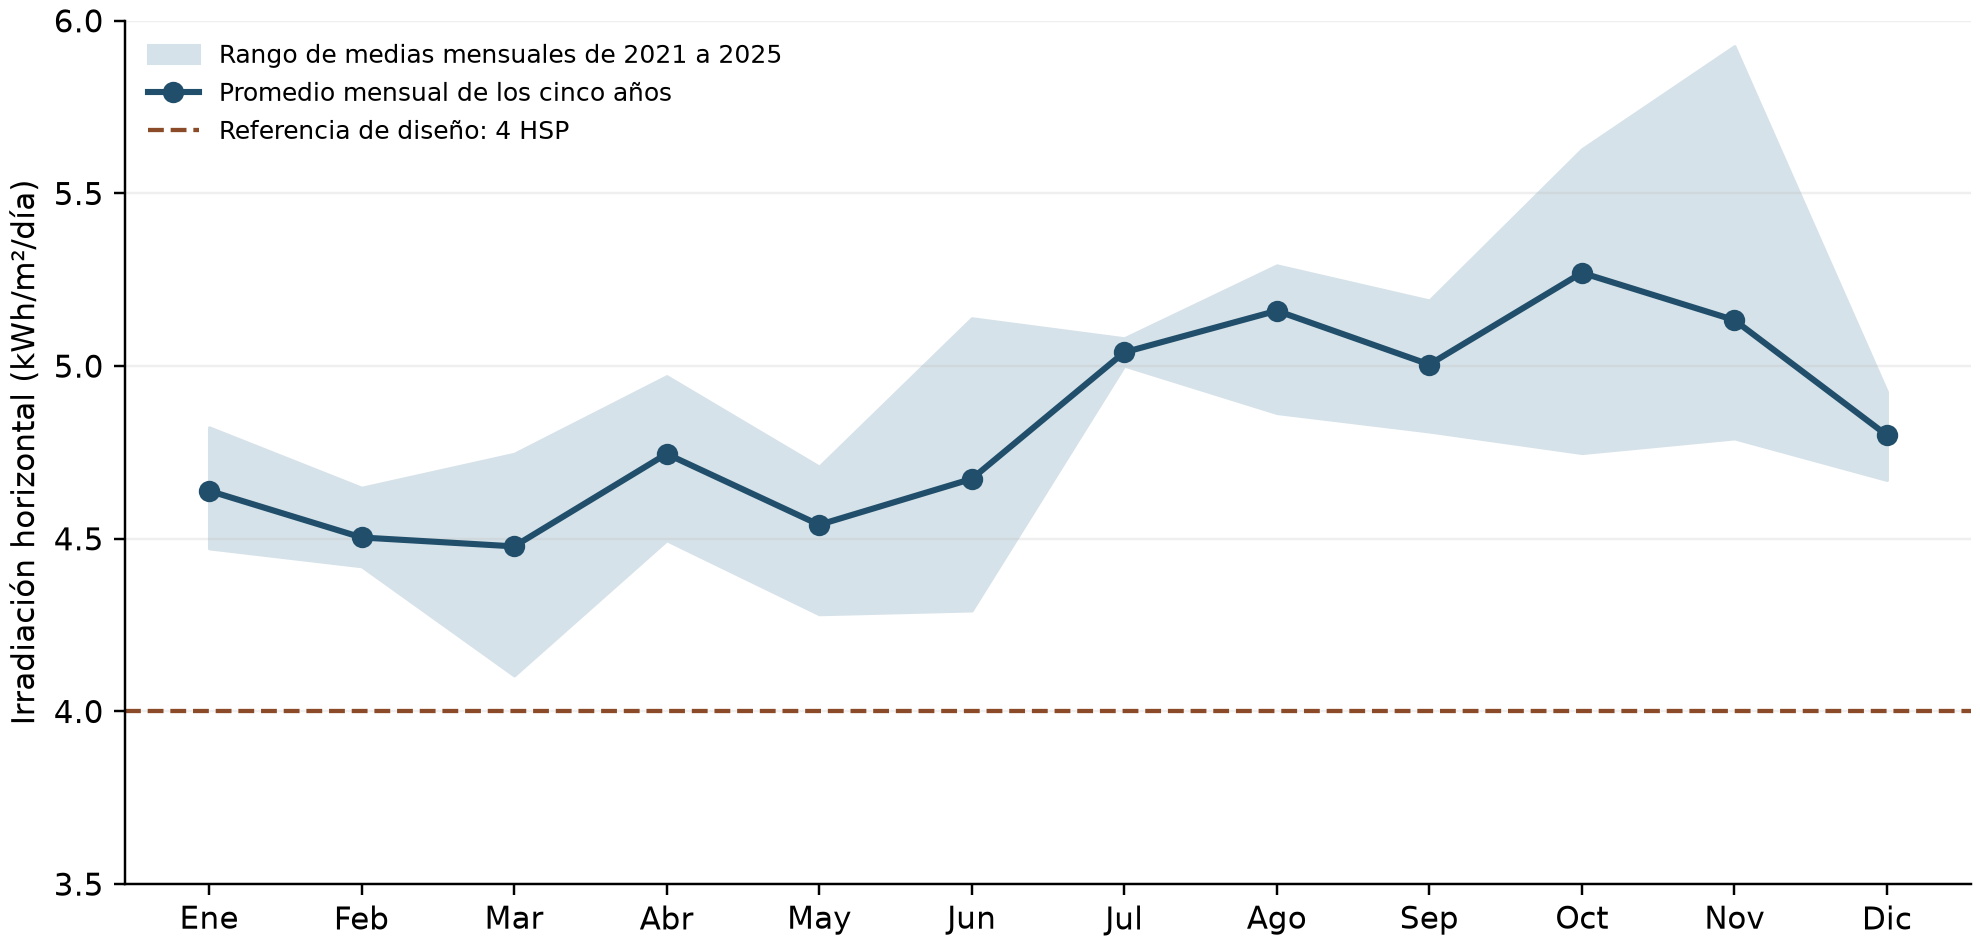
\includegraphics[width=\linewidth]{imagenes/recurso_solar_nasa.png}\par
\captionof{figure}{Recurso solar regional de referencia, NASA POWER 2021 a 2025}\label{fig:recurso}
\end{center}
La serie es un producto regional, no una medición de cubierta. La ingeniería incorporará coordenadas y cota del sitio, orientación, inclinación, sombras e irradiación sobre el plano de módulos. La aproximación horizontal se utiliza para el balance de formulación; las medias mensuales no describen cada día de nubosidad.
\subsection{Balance energético de formulación}
El cuadro \ref{tab:energia} fija supuestos de cálculo. La potencia del terminal completo deberá reemplazarse por ficha o medición con el brillo, cliente y periféricos reales.

\cuadro{tab:energia}{Supuestos y resultados del escenario energético}{@{}Y P{4.5cm}@{}}{\textbf{Variable}&\textbf{Valor de formulación}}{
Terminales y consumo completo supuesto & 3 unidades de 200 W cada una\\*
Horario activo; apagado fuera de servicio & 12 h/día; 0 W restante supuesto\\
Comunicaciones y videovigilancia & 40 W, 24 h/día; desglose en el cuadro \ref{tab:cargas}\\
Potencia simultánea & $3(200)+40=640$ W\\
Energía diaria de cargas & $3(0,200)(12)+0,040(24)=8,16$ kWh/día\\
Energía para 4 horas de corte & $0,640(4)=2,56$ kWh AC\\
Generación propuesta para estudiar & $6(615)=3\,690$ Wp, es decir 3,69 kWp\\
Recurso y factor global supuestos & 4 HSP/día; factor 0,75\\
Producción ilustrativa & $3,69(4)(0,75)=11,07$ kWh/día\\
Sensibilidad con 3 HSP & 8,3025 kWh/día, antes de revisar auxiliares\\
}
HSP significa horas solares pico equivalentes. Los 4 HSP son una referencia conservadora respecto de las medias mensuales regionales; el factor 0,75 es un supuesto global de conversión. El diseño incorporará el plano de captación, las sombras y el periodo crítico. No se computa ganancia bifacial sin geometría y albedo comprobados, ni se añaden dos veces pérdidas ya incluidas en el factor.

El mínimo aritmético con margen de 20\% sería:
\[
N_{\mathrm{FV}}=\left\lceil\frac{1,20(8,16)}{0,615(4)(0,75)}\right\rceil=6.
\]
Si se incorpora como sensibilidad un consumo propio adicional de 15 W del inversor durante 24 h, la carga equivalente aumenta a 8,52 kWh/día. Ese consumo es también supuesto; se reemplazará por dato del equipo y se delimitarán las pérdidas. Con 3 HSP, los 8,3025 kWh/día no cubrirían dicho escenario: se demuestra la dependencia del recurso y del horario.

Para una batería nominal de 4,8 kWh, una profundidad de descarga de diseño de 80\%, capacidad remanente de 80\% y rendimiento batería a salida AC de 90\% permiten comprobar:
\[
E_{\mathrm{AC,diseño}}=4,8(0,80)(0,80)(0,90)=2,7648\ \mathrm{kWh}.
\]
El resultado supera 2,56 kWh con una holgura limitada; se deben descontar auxiliares y efectos de temperatura. No equivale a una garantía de cuatro horas. La capacidad de energía se relacionará con la tensión y los Ah de la referencia exacta.

\subsection{Condiciones del emplazamiento y del montaje}
La ingeniería contrastará cubierta, sombras, acceso, carga, anclajes e impermeabilización. La superficie geométrica de los seis módulos de referencia es 16,21 m$^2$ y su masa es 194,4 kg; el diseño añadirá estructura, separaciones y condiciones de trabajo seguro.

Se definirán estructura y tornillería, inclinación y orientación, conductores por corriente y recorrido, conectores compatibles y canalizaciones. El suministro incluirá seccionamiento, protección próxima a batería, sobrecorriente, sobretensiones, protección diferencial indicada, tierra, equipotencialidad y señalización según el diseño.

La instalación entregará unifilar, ajustes, metrado, registros de pruebas, manual y responsable de mantenimiento. Los siete enlaces de red y los recorridos del circuito crítico se conciliarán con las plantas y la accesibilidad del terminal; su metrado de partida figura en la sección \ref{sec:especificaciones}.

\subsection{Escalabilidad y flexibilidad}
El CMS identificará terminal, grupo y versión del paquete para permitir ampliaciones sin mezclar contenidos. Antes de aumentar unidades se probarán carga de publicación, almacenamiento, ancho de banda y soporte. El costo de expansión incluirá levantamiento por edificio, nuevos circuitos y capacidad editorial; no se obtiene multiplicando únicamente el precio de una pantalla.

La autorización de una segunda etapa considerará utilidad demostrada, contenidos vigentes, continuidad de las tres terminales, costo de operación y responsables. No se promete cobertura de toda la UNSAAC con la infraestructura del piloto.

\clearpage
\section{Especificaciones técnicas y dimensionamiento}\label{sec:especificaciones}
\subsection{Criterio de redacción del requerimiento}
Las especificaciones se redactan por desempeño, sin marca, modelo, fabricante ni procedencia. El Reglamento de la Ley N.° 32069 dispone que el requerimiento no incluya exigencias desproporcionadas ni descripciones que orienten la contratación hacia un producto, salvo una compatibilización aprobada \cite{compatibilizacion}. La compatibilización procede cuando la entidad posee equipamiento preexistente que debe complementarse; el piloto no tiene ese caso.

Cada especificación indica el valor mínimo, su propósito y la razón del valor elegido. Las marcas aparecen sólo en los cuadros comparativos de la sección \ref{sec:seleccion}, que contrastan las ofertas con estas especificaciones y eligen una referencia de valorización. El anexo C registra de qué documento se tomó cada característica. Una oferta de otra marca será aceptada si acredita con la ficha del fabricante el cumplimiento de todos los mínimos.

\cuadro{tab:et_resumen}{Especificaciones técnicas del requerimiento}{@{}P{1.3cm}P{4.6cm}P{1.6cm}Y@{}}{\textbf{Código}&\textbf{Bien o servicio}&\textbf{Cantidad}&\textbf{Propósito}}{
ET-01 & Terminal interactivo de consulta & 3 & Consulta táctil en los tres pisos\\*
ET-02 & Plataforma central de contenidos y base de datos & 1 servicio & Edición, aprobación, distribución y respaldo\\
ET-03 & Red local y cableado estructurado & 7 enlaces & Conexión de terminales, NVR y enlace institucional\\
ET-04 & Videovigilancia de los terminales & 3 cámaras, 1 NVR & Protección de los equipos y evidencia de incidentes\\
ET-05 & Inversor híbrido con cargador & 1 & Conversión FV, carga de batería y respaldo\\
ET-06 & Módulos fotovoltaicos & 6 & Generación de 3,69 kWp\\
ET-07 & Batería de litio con BMS & 1 & Cuatro horas de autonomía de cargas críticas\\
ET-08 & Estructura de montaje FV & 2 conjuntos & Fijación segura en la cubierta\\
ET-09 & Protecciones, tablero, conductores y tierra & 1 sistema & Seguridad eléctrica DC y AC\\
ET-10 & Medición y monitoreo energético & 1 conjunto & Exportación cero y registro de energía\\
}

\subsection{Decisiones de dimensionamiento}
El cuadro \ref{tab:decisiones} explica por qué se adopta cada cantidad o capacidad y no un valor menor o mayor. Los cálculos de respaldo se desarrollan en las subsecciones siguientes y en el balance energético.

\cuadrolargo{tab:decisiones}{Por qué se adopta cada valor y no otro}{@{}P{2.4cm}P{2.6cm}P{1.8cm}Y@{}}{\textbf{Decisión}&\textbf{Alternativas evaluadas}&\textbf{Valor adoptado}&\textbf{Razón}}{
Número de terminales & 2, 3 o 6 & 3 & Uno por piso cubre las tres zonas de tránsito de los planos; 2 deja un piso sin punto de consulta y 6 duplica inversión y energía sin demanda medida\\*
Tamaño de pantalla & 43, 55 o 65 pulgadas & 55 & 43 pulgadas reduce el área de lectura en 39\%; 65 la aumenta en 40\%, pero también masa, consumo, precio y obstrucción del pasillo\\
Resolución & FHD o 4K & 4K & Texto nítido en formato vertical a 1 a 3 m; las ofertas de 55 pulgadas ya la incluyen\\
Brillo & 350, 400 a 500 o más de 700 cd/m\textsuperscript{2} & 400 mínimo & Suficiente en interior; los paneles de más de 700 cd/m\textsuperscript{2} se destinan a vitrinas y elevan el consumo\\
Memoria RAM & 4, 8, 16 o 32 GB & 8 mínimo; 16 de referencia & 4 GB es el mínimo de Windows 11 y no deja margen al reproductor 4K; 16 GB ya viene en las ofertas comparadas; 32 GB no tiene carga que lo justifique\\
SSD del terminal & 128, 256 o 512 GB & SSD de 256 GB & Sistema, actualizaciones y biblioteca local necesitan unos 96 GB con 25\% libre; 256 GB es la menor capacidad ofrecida y 512 GB no aporta uso\\
Cámaras & 0, 3 o 6 & 3 & Una por terminal cubre equipo y usuario; sin cámaras el riesgo de daño queda sin evidencia; 6 duplica costo y datos personales sin necesidad\\
Canales del NVR & 4, 8 o 16 & 4 & Tres cámaras más una reserva; 8 o 16 canales pagan capacidad ociosa\\
Disco de grabación & 1, 2 o 4 TB & 2 TB & 30 días requieren unos 1\,069 GB; 1 TB no alcanza y 4 TB supera el plazo de conservación\\
Cable de red & Cat 5e, Cat 6 o Cat 6A; cobre o CCA & Cat 6 de cobre LSZH & Gigabit con margen a 250 MHz; Cat 6A sirve a 10 Gb/s, no requerido; CCA no es cobre y se calienta con PoE; LSZH por recorrer vías de evacuación\\
Puertos del switch & 5, 8, 16 o 24 & 8 & Seis puertos usados y dos libres; 5 puertos no alcanza y 16 o 24 sólo agregan costo y consumo\\
Servidor del CMS & Físico propio, VM o VPS & VM institucional o VPS & Tres pantallas no justifican comprar y mantener un servidor; 2 vCPU, 8 GB y 100 GB cubren el cálculo con margen doble\\
Inversor & 3, 4, 5 o 6 kW & 4 kW, 16 A por MPPT & La carga es de 640 W; el criterio decisivo es la corriente del módulo de 15,15 A y la operación a 3\,400 m, que el modelo de 3 kW comparado no cumple\\
Batería & 2,4; 4,8 o 9,6 kWh & 4,8 kWh & 2,4 kWh entrega 1,38 kWh de diseño, 2,2 horas; 4,8 kWh entrega 2,76 kWh, 4,3 horas; 9,6 kWh duplica costo para 8,6 horas no requeridas\\
Módulos FV & 5, 6 u 8 & 6 & Con 4 HSP y factor 0,75, cinco módulos generan 9,23 kWh/día, por debajo de los 9,79 kWh/día requeridos; seis generan 11,07; ocho ocupan más cubierta sin necesidad\\*
}

\subsection{ET-01 Terminal interactivo de consulta}
\cuadro{tab:et01}{ET-01: terminal interactivo de consulta, tres unidades}{@{}P{2.7cm}Y Y@{}}{\textbf{Parámetro}&\textbf{Mínimo exigido}&\textbf{Propósito y sustento}}{
Formato & Tótem vertical de piso con pantalla de 55 pulgadas $\pm$1, base anclable y acceso técnico con llave & Lectura a 1 a 3 m en pasillos y protección contra manipulación\\*
Pantalla & 3\,840 $\times$ 2\,160 en vertical; brillo de 400 cd/m\textsuperscript{2} como mínimo, preferible 450 a 500 & Texto legible bajo iluminación interior y reflejos moderados\\
Superficie táctil & Infrarroja o capacitiva, 10 contactos simultáneos como mínimo, vidrio protector & Consulta por una o dos personas sin pérdida de respuesta\\
Procesador & x86-64 de 4 núcleos o más incluido en la lista de procesadores admitidos por Windows 11, con decodificación 4K por hardware; o SoC Android con reproductor soportado & Reproductor, navegador y actualizaciones sin exigir gama máxima \cite{win11cpu}\\
Memoria y almacenamiento & RAM de 8 GB como mínimo; SSD de 256 GB, durabilidad declarada de 100 TBW o más & Cinco años de escritura estimada suman 3,7 TB, muy por debajo de la durabilidad exigida\\
Sistema operativo & Windows 11 Pro o equivalente con licencia y bloqueo de kiosco; Android 13 o superior si se elige esa ruta & Soporte de seguridad durante el horizonte; Windows 10 no se acepta \cite{win10fin}\\
Conectividad & Ethernet RJ45 Gigabit; Wi-Fi opcional & Enlace estable por cable, ET-03\\
Energía & 220 V, 60 Hz; potencia máxima declarada del conjunto de 200 W o menos & Cota del balance energético; mayor consumo obliga a recalcular\\
Ambiente & Operación entre 0 y 40\,°C; aptitud a 3\,400 m declarada o demostrada & Condiciones de Cusco\\
Garantía & 1 año como mínimo con atención en Cusco; preferible 3 años & Continuidad del piloto y repuestos\\
}
La memoria de 8 GB es el mínimo exigido y 16 GB la referencia de las ofertas. El SSD se dimensiona así: Windows 11 exige 64 GB, la biblioteca local del reproductor ocupa unos 11 GB y los registros 2 GB. El total de 77 GB, con 25\% de espacio libre, da unos 96 GB. Las ofertas comparadas parten de 256 GB sin diferencia de precio; 512 GB no tendría uso en el horizonte. Se exige durabilidad y no la marca del SSD: con unos 2 GB escritos al día, cualquier unidad de consumo general con 100 TBW resiste más de cien años de esa carga.

\subsection{ET-02 Plataforma central de contenidos y base de datos}
\cuadro{tab:et02}{ET-02: plataforma central de contenidos y base de datos}{@{}P{2.7cm}Y Y@{}}{\textbf{Parámetro}&\textbf{Mínimo exigido}&\textbf{Propósito y sustento}}{
Despliegue & Máquina virtual institucional o servidor privado virtual con sistema Linux de soporte extendido y contenedores & Separar plataforma y terminales; actualizar sin tocar el kiosco\\*
Procesamiento & 2 vCPU y 8 GB de RAM & Tres destinos y pocos editores concurrentes; ver cálculo\\
Almacenamiento & SSD o NVMe de 100 GB & Biblioteca, base de datos, registros y copias locales con margen doble\\
Base de datos & Motor relacional que exija la versión del CMS, con copia transaccional diaria & Integridad de avisos, versiones y auditoría\\
Copias & Diarias, retención de 30 días y una copia fuera del servidor, cifrada & RPO de 24 h y restauración ensayada\\
Acceso & HTTPS con certificado válido; administración con cuentas individuales y segundo factor o VPN & Seguridad del servicio público\\
Transferencia & 1 TB/mes como mínimo & Descarga de paquetes de las tres terminales\\
}
\cuadro{tab:et02_calculo}{Cálculo de capacidad de la plataforma central}{@{}Y r P{5.2cm}@{}}{\textbf{Componente}&\textbf{Estimación}&\textbf{Base}}{
Sistema operativo y contenedores & 20 GB & Imagen base, CMS, servidor web y mensajería\\*
Biblioteca de medios & 12 GB & 500 avisos de 2 MB y 30 videos de 150 MB, con dos versiones\\
Base de datos y registros & 4 GB & Doce meses de avisos, auditoría y estado de terminales\\
Copias locales & 14 GB & Siete días de copia antes de su envío externo\\\midrule
\textbf{Total con margen doble} & \textbf{100 GB} & 50 GB estimados $\times$ 2 por crecimiento\\
Memoria & 8 GB & 6 GB estimados: sistema 1, base de datos 2, CMS 2, caché y mensajería 1\\
}
Un servidor físico propio exigiría compra, espacio, energía, reposición y soporte para sólo tres pantallas. La alternativa elegida y su costo se comparan en la sección \ref{sec:seleccion}.

\subsection{ET-03 Red local y cableado estructurado}
\cuadro{tab:et03}{ET-03: red local y cableado estructurado}{@{}P{2.7cm}Y Y@{}}{\textbf{Parámetro}&\textbf{Mínimo exigido}&\textbf{Propósito y sustento}}{
Cable & Categoría 6 U/UTP de cobre sólido de 23 o 24 AWG, chaqueta LSZH; no se acepta CCA & Gigabit y PoE sin calentamiento; menor emisión de humo en vías de evacuación\\*
Longitud & Enlace permanente de 90 m como máximo y canal de 100 m & Límite del cableado de cobre; los recorridos estimados no superan 50 m\\
Terminación & Jack keystone Cat 6 en ambos extremos, faceplate, patch panel y patch cords Cat 6 & Enlaces sustituibles y certificables\\
Identificación & Etiqueta en ambos extremos y plano de recorridos & Mantenimiento y diagnóstico\\
Switch & 8 puertos 10/100/1000 administrables, VLAN IEEE 802.1Q, QoS, gestión web o SNMP y al menos un puerto de enlace & Separar terminales, cámaras y administración\\
Gabinete & De pared, 6 RU, con puerta y llave, bandeja, organizador y regleta & Proteger equipos activos en el circuito crítico\\
Canalización & Canaleta de PVC con tapa o tubería, sin cables expuestos en zonas de tránsito & Seguridad y orden\\
Pruebas & Mapa de cableado, continuidad y longitud de cada enlace, con registro & Aceptación PE5\\
}
\cuadro{tab:metrado_red}{Metrado de partida del cableado de red}{@{}P{1.0cm}Y r@{}}{\textbf{ID}&\textbf{Enlace desde el gabinete del tercer piso}&\textbf{Metros}}{
L1 & Terminal del primer piso & 45\\*
L2 & Terminal del segundo piso & 30\\
L3 & Terminal del tercer piso & 15\\
L4 & Cámara del primer piso & 48\\
L5 & Cámara del segundo piso & 33\\
L6 & Cámara del tercer piso & 18\\
L7 & Enlace al punto de red institucional & 20\\\midrule
& Subtotal de recorridos & 209\\
& Holgura de 10\% por trazado y 2 m de reserva por enlace & 35\\
& \textbf{Total estimado frente a una caja de 305 m} & \textbf{244}\\
}
El gabinete se ubica en el tercer piso, junto al tablero crítico y al banco, para acortar el recorrido DC desde la cubierta. Las distancias son de partida y se medirán en el levantamiento. Una caja de 305 m cubre el total con 61 m de reserva; una segunda caja sólo se justificaría si el levantamiento superara ese valor. Se prevén 53 tramos de canaleta de 2 m para el 50\% del recorrido que no tenga canalización existente.

El switch usa seis puertos: enlace institucional, tres terminales, NVR y monitoreo del inversor. Quedan dos libres, es decir 25\% de reserva. Las cámaras se conectan a los puertos PoE propios del NVR. Así su red queda separada de la red de consulta y el switch no necesita entregar potencia.

\subsection{ET-04 Videovigilancia de los terminales}
La videovigilancia protege equipos de unos S/ 10\,000 cada uno, ubicados en zonas de tránsito libre, y aporta evidencia ante daños o hurto, riesgo R11. No se usa para controlar asistencia ni identificar usuarios del servicio y no incluye reconocimiento facial. Se aplicará la normativa de protección de datos personales y la directiva de la autoridad nacional sobre videovigilancia: aviso visible, finalidad limitada, acceso restringido y conservación por un plazo determinado \cite{datos}. El diseño fija 30 días, plazo que se confirmará con la norma vigente.

\cuadro{tab:et04}{ET-04: videovigilancia de los terminales}{@{}P{2.7cm}Y Y@{}}{\textbf{Parámetro}&\textbf{Mínimo exigido}&\textbf{Propósito y sustento}}{
Cámara & IP de 4 MP, 2\,560 $\times$ 1\,440; lente de 2,8 mm; H.265; IR de 20 m o más; PoE IEEE 802.3af; 6 W como máximo; ONVIF & Ver el terminal y su entorno a 2 a 5 m, también con baja luz\\*
Grabador & NVR de 4 canales o más con 4 puertos PoE, 40 Mbps de entrada como mínimo, 1 bahía SATA y usuarios con permisos & Grabación local en el circuito con respaldo\\
Disco & De videovigilancia, uso continuo, 2 TB & 30 días de conservación según el cálculo\\
Grabación & Continua en horario de servicio y por evento fuera de él; hora sincronizada & Evidencia con fecha válida y menor almacenamiento\\
Acceso & Cuentas individuales, registro de consultas y exportación sólo por solicitud autorizada & Protección de datos personales\\
Señalización & Un aviso por ubicación & Información al titular de los datos\\
}
\cuadro{tab:cctv_calculo}{Cálculo de grabación, ancho de banda y potencia}{@{}Y r P{5.0cm}@{}}{\textbf{Magnitud}&\textbf{Resultado}&\textbf{Base}}{
Grabación continua en servicio & 32,4 GB/día & 3 cámaras $\times$ 2 Mbps $\times$ 12 h\\*
Grabación por evento fuera de servicio & 3,2 GB/día & 10\% de actividad en las 12 h restantes\\
Conservación de 30 días & 1\,069 GB & (32,4 + 3,2) $\times$ 30\\
Ocupación de un disco de 2 TB & 53\% & 1\,069 GB entre 2\,000 GB\\
Alternativa de grabación continua 24 h & 1\,944 GB & Dejaría el disco al 97\%, sin margen\\
Ancho de banda de entrada & 12 Mbps & 3 cámaras $\times$ 4 Mbps de pico, frente a 40 Mbps exigidos\\
Potencia PoE & 12,9 W & 3 cámaras $\times$ 4,3 W de la opción elegida\\
}
La tasa de 2 Mbps corresponde a una escena interior estática con H.265 y se medirá en el ensayo. Si resultara mayor, se reducirá la grabación continua o se ajustará el disco antes de aceptar el sistema.

\subsection{ET-05 a ET-08 Subsistema fotovoltaico}
\cuadro{tab:et05}{ET-05: inversor híbrido con cargador}{@{}P{2.7cm}Y Y@{}}{\textbf{Parámetro}&\textbf{Mínimo exigido}&\textbf{Propósito y sustento}}{
Salida & Monofásica 220 a 230 V, 60 Hz; 3 kW nominales como mínimo & 640 W de carga simultánea con margen para transitorios y ampliación\\*
Respaldo & Salida de 3 kVA como mínimo; conmutación de 20 ms o menos & Las terminales no deben reiniciarse en un corte\\
Entrada FV & 2 MPPT; 16 A de entrada y 20 A de cortocircuito por MPPT como mínimo; tensión máxima de 500 V o más & Imp de 15,15 A e Isc de 16,02 A del módulo; Voc de la cadena en frío de 318,94 V\\
Batería & Litio de baja tensión, 48 V; 60 A de carga y descarga como mínimo; BMS por CAN o RS485 & Banco ET-07 con protección coordinada\\
Altitud & 3\,500 m o más, con reducción de potencia documentada si corresponde & Cusco se ubica cerca de 3\,400 m\\
Otros & IP65 o más; eficiencia máxima de 97\% o más; control de exportación cero con medidor; monitoreo & Instalación interior protegida y registro\\
Garantía & 5 años como mínimo & Horizonte del piloto\\
}
\cuadro{tab:et0608}{ET-06 a ET-08: módulos, batería y estructura}{@{}P{2.7cm}Y Y@{}}{\textbf{Elemento}&\textbf{Mínimo exigido}&\textbf{Propósito y sustento}}{
ET-06 Módulos & 600 Wp o más; eficiencia de 21\% o más; Imp no mayor que la corriente del MPPT; garantía de producto de 12 años y de potencia de 25 años & Seis unidades para 3,69 kWp en 16,2 m$^2$\\*
ET-07 Batería & LiFePO4 de 48 a 51,2 V; 4,8 kWh nominales; profundidad de 80\% o más; 6\,000 ciclos al 80\% o más; 60 A continuos; carga de 0 a 45\,°C como mínimo; BMS compatible documentado; garantía de 5 años; UN38.3 & 2,76 kWh de diseño para 2,56 kWh de cuatro horas\\
ET-08 Estructura & Aluminio anodizado o acero galvanizado; inclinación de 10 a 20° hacia el norte; compatible con módulos de 2\,382 $\times$ 1\,134 mm; fijación sin dañar la impermeabilización; cálculo de viento & Cusco está a 13,5° S; 15° favorece la autolimpieza con lluvia\\
}

\subsection{ET-09 y ET-10 Protecciones, conductores, tierra y medición}
\cuadro{tab:et0910}{ET-09 y ET-10: protecciones, tablero, conductores, tierra y medición}{@{}P{3.1cm}P{4.4cm}Y@{}}{\textbf{Elemento}&\textbf{Mínimo exigido}&\textbf{Sustento del valor}}{
Seccionamiento DC & Interruptor de 25 A y 600 V DC como mínimo & 1,25 $\times$ Isc de 16,02 A da 20,0 A; tensión en frío de 318,94 V\\*
Sobretensiones DC & Protector 2P de 600 V DC, 20 a 40 kA & Descargas en la cubierta\\
Fusible de cadena & No requerido con una cadena por MPPT & Sólo se exige con tres o más cadenas en paralelo\\
Cable FV & 6 mm² de 1,5 kV para uso solar, con conectores MC4 & Caída de 0,54\% en 15 m\\
Batería & Cable de 35 mm² y fusible de 150 A & 100 A de descarga máxima por 1,25 da 125 A; 150 A es el valor comercial siguiente y el cable lo admite\\
Entrada de red y salida de respaldo & Termomagnéticos 2P de 32 A con conductor de 6 mm² & Entrada máxima del inversor de 27,3 A y salida de respaldo de 21,7 A\\
Circuitos derivados & Dos termomagnéticos 2P de 16 A, uno para terminales y otro para red y cámaras, con diferencial de 30 mA cada uno & Carga de 2,73 A y 0,2 A; protección de personas\\
Sobretensiones AC & Protector tipo 2 de 275 V y 40 kA & Equipos electrónicos sensibles\\
Tablero & Adosable de 18 polos con riel DIN & 14 polos ocupados y 4 de reserva\\
Conductores AC & LSZH de 2,5 mm² en circuitos derivados & Caída de 0,78\% en 45 m\\
Puesta a tierra & Pozo con barra de cobre de 5/8 pulg. $\times$ 2,4 m, cemento conductivo y conductor de 10 mm²; resistencia de 25 $\Omega$ o menos & Referencia del CNE, Utilización \cite{cne}; medición con telurómetro\\
ET-10 Medición & Medidor bidireccional monofásico Modbus RS485 compatible con el inversor; monitoreo con registro exportable & Exportación cero y separación de energía FV, red, batería y cargas\\
}
\cuadro{tab:caida_tension}{Comprobación de caída de tensión}{@{}P{3.2cm}Y r r@{}}{\textbf{Tramo}&\textbf{Datos}&\textbf{Caída V}&\textbf{\%}}{
Cadena FV al inversor & 6 mm², 15 m de ida, 15,15 A, 243,6 V & 1,33 & 0,54\\*
Batería al inversor & 35 mm², 2 m de ida, 100 A, 51,2 V & 0,20 & 0,39\\
Circuito de terminales & 2,5 mm², 45 m de ida, 2,73 A, 220 V & 1,72 & 0,78\\
Circuito de red y cámaras & 2,5 mm², 5 m de ida, 0,2 A, 220 V & 0,01 & 0,00\\
}
La caída se calcula con $\Delta V = 2LI\rho/S$ y $\rho = 0,0175\ \Omega\,\mathrm{mm^2/m}$. El criterio de diseño adoptado es de 1,5\% en DC y 2,5\% en circuitos AC derivados; todos los tramos lo cumplen con holgura. El profesional responsable confirmará secciones, recorridos y protecciones en el diseño ejecutivo.

\subsection{Cuadro de cargas eléctricas por equipo}
\cuadro{tab:cargas}{Cuadro de cargas del circuito crítico}{@{}P{3.6cm}r r r r Y@{}}{\textbf{Equipo}&\textbf{Cant.}&\textbf{W c/u}&\textbf{h/día}&\textbf{Wh/día}&\textbf{Fuente del valor}}{
Terminal interactivo & 3 & 200,0 & 12 & 7\,200 & Cota de diseño ET-01\\*
Cámara IP & 3 & 4,3 & 24 & 310 & Ficha de la opción elegida\\
NVR con disco & 1 & 12,0 & 24 & 288 & Cota; 4,25 W publicados sin disco en una opción comparada\\
Switch administrable & 1 & 10,0 & 24 & 240 & Cota; sin carga PoE\\
Medidor y monitoreo & 1 & 2,0 & 24 & 48 & Cota\\
Reserva de comunicaciones & 1 & 3,1 & 24 & 74 & Completa la cota de 40 W\\\midrule
\textbf{Subtotal} & & 640,0 & & \textbf{8\,160} & 600 W de terminales y 40 W de comunicaciones\\
Autoconsumo del inversor & 1 & 15,0 & 24 & 360 & Supuesto; la ficha no lo publica\\\midrule
\textbf{Total del escenario} & & 655,0 & & \textbf{8\,520} & Coincide con el balance energético\\
}
Los equipos de comunicación identificados suman 36,9 W y 886 Wh/día; la reserva de 3,1 W completa la cota de 40 W usada en el balance. El total de 8,52 kWh/día es el mismo escenario del cuadro \ref{tab:energia}. Las cotas sin ficha se reemplazarán por la medición del ensayo.

\subsection{Mantenimiento de pantallas, equipos y sistema FV}
El mantenimiento se planifica por equipo y no sólo como una partida global. El cuadro \ref{tab:mant_detalle} fija la actividad, la frecuencia, el responsable y su base de costo. Los importes anuales alimentan la partida de mantenimiento del cuadro \ref{tab:opex}.

\cuadrolargo{tab:mant_detalle}{Plan de mantenimiento por equipo}{@{}P{2.4cm}Y P{2.2cm}P{2.6cm}@{}}{\textbf{Equipo}&\textbf{Actividad}&\textbf{Frecuencia}&\textbf{Responsable}}{
Pantalla y vidrio & Limpieza con el equipo apagado, paño de microfibra y limpiador sin amoníaco ni abrasivos; nunca rociar sobre la pantalla & Diaria o según uso & Operación local\\*
Marco táctil & Retirar polvo de los sensores, comprobar 10 contactos y calibrar si hay desvío & Mensual & TI\\
Interior del tótem & Polvo en ventiladores y rejillas, conexiones, temperatura interna y estado SMART del SSD & Semestral & Técnico\\
Software del terminal & Actualizaciones de sistema, controladores y reproductor en ventana programada, con retorno & Mensual & TI\\
Uso del panel & Apagado fuera de horario y rotación de contenido para evitar imagen fija prolongada & Programado en el CMS & TI y editores\\
Cámaras y NVR & Limpieza del domo, hora sincronizada, grabación y ocupación del disco & Mensual & TI\\
Red & Puertos, etiquetas, patch cords y registro del switch & Semestral & TI\\
Módulos FV & Limpieza con agua sin detergentes abrasivos, temprano; conectores y estructura & Semestral & Personal competente\\
Inversor y batería & Alarmas, temperatura, estado de carga y salud, firmware & Mensual por monitoreo & Responsable técnico\\
Tablero y tierra & Ajuste de bornes, prueba del diferencial y medición de la resistencia de tierra & Anual & Electricista competente\\*
}
\cuadro{tab:mant_costo}{Costo anual del mantenimiento local y energético}{@{}Y P{5.2cm}r r@{}}{\textbf{Concepto}&\textbf{Base}&\textbf{A1 S/}&\textbf{A2 S/}}{
Insumos de limpieza & Paños, limpiador y elementos de protección & 140,00 & 140,00\\*
Mantenimiento preventivo de terminales & 2 visitas $\times$ 3 terminales $\times$ 1 h $\times$ S/ 60 & 360,00 & 360,00\\
Limpieza y revisión FV & 2 visitas $\times$ 2 h $\times$ S/ 50 & 0,00 & 200,00\\\midrule
\textbf{Total anual} & & \textbf{500,00} & \textbf{700,00}\\
}
Las revisiones de cámaras, NVR, red y software forman parte de las 48 HP anuales de soporte TI. La medición de tierra y la prueba del diferencial se realizan en la visita preventiva. Los repuestos críticos son patch cords, jacks, un disco de reserva cuando el uso lo justifique, conectores MC4 y fusibles; se adquirirán con cargo a la contingencia o a la reposición cuando se identifique la falla.

\section{Selección de referencias de mercado}\label{sec:seleccion}
\subsection{Método de comparación y elección}
Cada cuadro de esta sección compara opciones publicadas en Perú contra la especificación ET correspondiente. La ficha del fabricante respalda las características y la página del proveedor respalda precio, IGV y stock. Se marca \textbf{C} cuando la característica cumple y está documentada, \textbf{P} cuando falta acreditarla y \textbf{N} cuando no cumple.

La regla de elección es la misma en todos los casos: entre las opciones sin N, se elige la de menor costo total; ante costos cercanos, prevalece la que tiene más características documentadas. La opción elegida sólo fija el valor referencial del presupuesto. El requerimiento sigue siendo genérico y cualquier equivalente que cumpla puede ofertar. Los precios se consultaron el 30 de octubre de 2026, incluyen IGV salvo indicación y el anexo C registra la procedencia de cada dato.

Los proveedores de energía y de red son AutoSolar Perú, que publica precios con IGV incluido, y ARTEUS S.A.C., RUC 20608279637, cuyos términos indican que los precios incluyen IGV \cite{arteus}. Panacompu Perú se usó sólo como contraste, porque su página indica que no acepta pedidos en Perú durante el traslado de su almacén \cite{panacompu}.

\subsection{Inversor híbrido, ET-05}
\begin{table}[htbp]\formatofichas
\caption{Inversores híbridos analizados como opción frente a ET-05}\label{tab:comp_inversor}
\begin{tabularx}{\linewidth}{@{}>{\raggedright\arraybackslash}p{2.25cm}YYYYY@{}}
\toprule
\textbf{Característica} & \textbf{Tensite AH4M-2} & \textbf{Solis S6-EH1P3K-L} & \textbf{Suntaic STH6M-2/GEN} & \textbf{Livoltek Hyper-5000} & \textbf{Growatt SPH3000}\\\midrule
Potencia nominal & 4\,000 W & 3\,000 W & 6\,000 W & 5\,000 W & 3\,000 W\\
MPPT y corriente por MPPT & 2; 16 A & 2; 16 A & 2; 15 A & 2; 14 A & 2; 12 A\\
Cortocircuito por MPPT & 20 A & 24 A & 18 A & 17,5 A & No publicado\\
Tensión FV máxima; rango MPPT & 550 V; 40 a 530 V & 600 V; 90 a 520 V & 550 V; 90 a 500 V & 600 V; 125 a 550 V & 550 V; 150 a 550 V\\
Batería; corriente & 48 V, 40 a 60 V; 100 A & 42 a 58 V; 62,5 A & 42 a 59 V; 100 A & 40 a 60 V; 100 A & 42 a 59 V; 66 A\\
Respaldo & 5\,000 VA; 10 ms & 3\,000 W & 6\,000 VA & 5\,000 W & 3\,000 W\\
Eficiencia; IP & 97,6\%; IP66 & Por verificar & 98\%; IP65 & 97,8\%; IP65 & Cerca de 98\%; IP65\\
Altitud de operación & 4\,000 m; reducción sobre 3\,000 m & Por verificar & 3\,000 m & No publicada & Por verificar\\
Garantía & 10 años de producto & Por verificar & No publicada & No publicada & 5 años, ampliable a 10\\
Precio con IGV & S/ 6\,537,03; sin IGV S/ 5\,539,86 & Sin precio publicado en Perú & S/ 4\,077,77 con 15\% de descuento & S/ 2\,960,94 & S/ 8\,368,82\\\midrule
Corriente frente a 15,15 A & \textbf{C} & \textbf{C} & \textbf{N}: limita la cadena & \textbf{N}: limita la cadena & \textbf{N}: limita la cadena\\
Altitud frente a 3\,400 m & \textbf{C} & \textbf{P} & \textbf{N} & \textbf{P} & \textbf{P}\\
\textbf{Resultado} & \textbf{Elegida} & Sin precio verificable & No cumple ET-05 & No cumple ET-05 & No cumple ET-05\\
\bottomrule
\end{tabularx}
\fuentefichas{Páginas de AutoSolar Perú y fichas técnicas enlazadas en ellas, consultadas el 30 de octubre de 2026 \cite{tensiteinv,suntaicinv,livoltek,growattsph}; Solis según su manual y ficha global \cite{solismanual2025,solisglobal2024}. La corriente de 15,15 A es la Imp STC del módulo elegido.}
\end{table}
El cuadro \ref{tab:comp_inversor} muestra que el precio más bajo no define la elección. Los modelos de 5 y 6 kW cuestan menos que el elegido, pero admiten 14 y 15 A por seguidor: con módulos de 15,15 A recortarían la producción en cada hora de sol. El modelo de 6 kW declara además 3\,000 m de altitud, por debajo de la cota de Cusco. El de 3 kW admite sólo 12 A y es el más caro. La referencia del informe anterior cumple la corriente, pero no tiene precio publicado en Perú ni altitud verificada. \textbf{Se elige el inversor de 4 kW} por cumplir corriente, altitud y batería de 48 V con ficha completa, stock y diez años de garantía.

\subsection{Batería, ET-07}
\cuadro{tab:comp_bateria}{Baterías LFP de 48 V analizadas como opción frente a ET-07}{@{}P{2.4cm}YYYY@{}}{\textbf{Característica}&\textbf{Tensite TS-L5000/LV}&\textbf{Pylontech US5000}&\textbf{Suntaic ST-L5000/LV}&\textbf{Felicity LPBF48100}}{
Energía total y útil & 4,8 kWh; 4,3 kWh & 4,8 kWh; profundidad 95\% & 5,22 kWh; 4,7 kWh & 5 kWh útiles\\*
Ciclos & Más de 6\,000 al 80\% & Más de 6\,000 al 95\% & No publicado & 6\,000 o más\\
Corriente & 60 A nominal; 100 A continuos & No publicado & 50 A nominal; 100 A máx. & No publicado\\
Temperatura de carga & 0 a 50\,°C & 0 a 50\,°C según manual & No publicado & No publicado\\
Comunicación & CAN y RS485 & CAN y RS485 & CAN y RS485 & CAN y RS485\\
Garantía & 5 años & 10 años & No publicado & No publicado\\
Compatibilidad con el inversor elegido & Mismo fabricante & Por acreditar & Por acreditar & Por acreditar\\
Precio con IGV & S/ 4\,178,47 & S/ 7\,493,00 en Sunperu; sin precio en AutoSolar & S/ 3\,535,17 con 28\% de descuento & S/ 3\,266,66\\\midrule
\textbf{Resultado} & \textbf{Elegida} & Mayor costo; compatibilidad P & Ficha incompleta; compatibilidad P & Sin ficha enlazada; IP21\\
}
Las dos baterías más baratas no publican ciclos o garantía y su compatibilidad con el inversor elegido no está documentada \cite{suntaicbat,felicity}. La de mayor garantía cuesta S/ 3\,314,53 más y tampoco acredita compatibilidad con ese inversor \cite{sunperuus5000,pylonas,us5000manual}. \textbf{Se elige la batería del mismo fabricante del inversor}, con ficha completa, temperatura, ciclos y certificaciones \cite{tensitebat}. Si una oferta acredita la compatibilidad de una batería más barata con ficha completa, se aceptará como equivalente y el ahorro reducirá la contingencia.

\subsection{Red, videovigilancia y almacenamiento, ET-03 y ET-04}
\cuadro{tab:comp_red}{Opciones de red y videovigilancia y opción elegida}{@{}P{2.2cm}Y P{2.6cm}Y@{}}{\textbf{Componente}&\textbf{Opciones comparadas, precio con IGV}&\textbf{Elegida}&\textbf{Razón}}{
Cámara IP de 4 MP & Dahua HDW1431T1P-S6, S/ 219; Dahua HDBW1431EN-S4, S/ 231; Dahua HDW2449T-S-IL, S/ 291 & HDW1431T1P-S6, S/ 219 & Menor precio con ficha completa: 2\,560 $\times$ 1\,440, 2,8 mm, H.265+, IR de 30 m, IP67, PoE 802.3af y 4,3 W; la tercera publica 1080p pese a su título\\*
NVR de 4 canales PoE & Dahua NVR1104HS-P-S3/H, S/ 292; TP-Link VIGI NVR1004H-4P, S/ 280; Dahua NVR2104HS-P-4KS3, S/ 335; Hilook NVR-104H-D/4P, S/ 227 & NVR1104HS-P-S3/H, S/ 292 & 4 puertos PoE, 80 Mbps y disco de hasta 8 TB; misma marca de las cámaras, sin depender de ONVIF; S/ 12 sobre la opción de menor precio con datos equivalentes\\
Switch de 8 puertos & D-Link DGS-1100-08P, S/ 327; Dahua S4210-8GT-110, S/ 517; Hikvision DS-3E1510P-SI, S/ 543; TP-Link SG2210MP, S/ 822 & S4210-8GT-110, S/ 517 & Menor precio entre los que documentan VLAN y gestión SNMP, con dos puertos de enlace; el de S/ 327 no publica 802.1Q y se aceptará si lo acredita\\
Cable Cat 6 de 305 m & CCA de 24 AWG, S/ 147; cobre de 24 AWG LSZH, S/ 666; cobre LSZH-1, S/ 667; LSZH sin conductor declarado, S/ 535 & Cobre de 24 AWG LSZH, S/ 666 & El CCA no es cobre y no cumple ET-03; entre los de cobre declarado, el de menor precio\\
Gabinete de pared & ZKTECO de 9 RU con bandeja, S/ 172; estándar de 6 RU, S/ 225; FINEN de 6 RU, S/ 117, sin stock verificable & ZKTECO de 9 RU, S/ 172 & Menor precio con stock verificable; incluye la bandeja y deja espacio de reserva\\
Disco de 2 TB & Seagate SkyHawk ST2000VX017, S/ 699, disponible; WD22PURZ, S/ 271, agotado; WD23PURZ, S/ 313,16 en Panacompu, sin pedidos en Perú & SkyHawk, S/ 699 & Único disco de videovigilancia de 2 TB con stock verificable; si se repone una opción más barata se aceptará como equivalente\\*
}
Las fuentes de los precios y modelos del cuadro \ref{tab:comp_red} son \cite{arteuscctv,arteusred,panacompu}. El anexo D presenta, como en una cotización, cada componente con imagen, características, precio y enlace, incluidos jacks, cajas, canaletas, tomacorrientes, conductores y protecciones. En cámaras, NVR, switch y disco, la elección no es la opción más barata en todos los casos. Lo es entre las que documentan los mínimos de la especificación, como pide la regla de elección.

\subsection{Alojamiento de la plataforma, ET-02}
\cuadro{tab:comp_hosting}{Opciones de alojamiento de la plataforma central}{@{}P{3.0cm}P{3.4cm}P{3.0cm}Y@{}}{\textbf{Opción}&\textbf{Recursos}&\textbf{Precio publicado}&\textbf{Observación}}{
Máquina virtual institucional & Según capacidad de TI & Sin compra & Preferente si TI la asigna con copias y soporte\\*
Hostinger KVM 2 & 2 vCPU, 8 GB, 100 GB NVMe & USD 8,79/mes por 24 meses; renueva a USD 14,99/mes & Cumple ET-02; precio de renovación conocido\\
Contabo Cloud VPS 4 & 4 vCPU, 8 GB, 100 GB SSD & EUR 4,40/mes por 24 meses & Cumple ET-02; requiere contrato de 24 meses y conversión desde euros\\
DigitalOcean Basic & 4 vCPU, 8 GiB, 160 GiB SSD & USD 48,00/mes & Cumple, con costo muy superior\\
Xibo Cloud Professional & CMS alojado por el fabricante & USD 4,90 por pantalla-mes & Sustituye el servidor, pero no el soporte local \cite{xibolic}\\
}
\textbf{Se elige la máquina virtual institucional} si TI la confirma. El presupuesto valoriza un servidor privado virtual equivalente con el precio de renovación de la opción KVM 2: USD 14,99 por 12 meses dan USD 179,88, es decir S/ 621,85 al tipo de cambio de 3,457 \cite{vps,bcrp}. La partida anual de S/ 720 cubre ese importe y S/ 98,15 para la copia externa. Se usa el precio de renovación y no el promocional, para no subestimar el costo del horizonte.

\subsection{Resumen de opciones elegidas}
\cuadro{tab:elegidas}{Opciones elegidas para valorizar el requerimiento}{@{}P{3.2cm}P{1.2cm}Y r P{1.4cm}@{}}{\textbf{Componente}&\textbf{ET}&\textbf{Opción elegida}&\textbf{Unitario S/}&\textbf{Cuadro}}{
Terminal interactivo & ET-01 & Prodimer TIPI7-55, i7 13.\textsuperscript{a} gen., 16 GB, 256 GB & 9\,499,99 & \ref{tab:fichas-totems}\\*
Plataforma central & ET-02 & Máquina virtual institucional o VPS equivalente & 720,00/año & \ref{tab:comp_hosting}\\
Cable de red & ET-03 & Cat 6 de cobre de 24 AWG LSZH, 305 m & 666,00 & \ref{tab:comp_red}\\
Switch & ET-03 & Dahua S4210-8GT-110 & 517,00 & \ref{tab:comp_red}\\
Gabinete & ET-03 & ZKTECO ZK-R9U-5409A con bandeja & 172,00 & \ref{tab:comp_red}\\
Tomacorriente & ET-03 & Bticino 2P+T de 16 A con placa & 39,35 & Anexo D\\
Cámara & ET-04 & Dahua IPC-HDW1431T1P-S6 & 219,00 & \ref{tab:comp_red}\\
NVR y disco & ET-04 & Dahua NVR1104HS-P-S3/H y SkyHawk de 2 TB & 991,00 & \ref{tab:comp_red}\\
Inversor híbrido & ET-05 & Tensite AH4M-2, 4 kW & 6\,537,03 & \ref{tab:comp_inversor}\\
Módulo FV & ET-06 & Jinko Tiger Neo de 615 Wp & 405,35 & \ref{tab:modulos_comparados}\\
Batería & ET-07 & Tensite TS-L5000/LV, 4,8 kWh & 4\,178,47 & \ref{tab:comp_bateria}\\
Estructura & ET-08 & Estructura inclinada de 15° para 3 módulos & 459,61 & \ref{tab:precios_energia}\\
Medición & ET-10 & Medidor SDM230 Modbus y módulo de monitoreo & 650,25 & \ref{tab:precios_energia}\\
}
Las marcas del cuadro \ref{tab:elegidas} no forman parte del requerimiento. La entidad las usará sólo para fijar el valor referencial y comprobar que el mercado ofrece bienes que cumplen.

\section{Evaluación económica y selección de alternativa}
\subsection{Base de estimación}
El análisis utiliza soles constantes de 2026 y un horizonte de cinco años. Se separan tres tipos de importe: precios publicados por proveedores identificados, estimaciones propias con base explícita y reservas condicionadas. La inversión comprende equipamiento, materiales, integración, instalación, pruebas y transferencia; la operación comprende soporte, alojamiento, mantenimiento, edición y energía.

Cada partida se valoriza con la opción elegida en la sección \ref{sec:seleccion} y se identifica por su especificación ET, no por la marca. Los precios se consultaron el 30 de octubre de 2026. Incluyen IGV, salvo el de los terminales, cuya página no lo declara y para el cual se mantiene una reserva tributaria. La configuración de compra se cerrará con la oferta técnica y económica del conjunto.

\subsection{Equipamiento con precio publicado}
\cuadro{tab:precios_energia}{Terminales y subsistema energético con precio publicado}{@{}Y r r r@{}}{\textbf{Partida}&\textbf{Cant.}&\textbf{Unitario S/}&\textbf{Parcial S/}}{
Tótem interactivo de 55 pulgadas, ET-01 & 3 & 9\,499,99 & 28\,499,97\\*\midrule
Módulo FV de 615 Wp, ET-06 & 6 & 405,35 & 2\,432,10\\
Inversor híbrido de 4 kW, ET-05 & 1 & 6\,537,03 & 6\,537,03\\
Batería LFP de 48 V y 4,8 kWh, ET-07 & 1 & 4\,178,47 & 4\,178,47\\
Medidor bidireccional Modbus, ET-10 & 1 & 502,41 & 502,41\\
Módulo de monitoreo del inversor, ET-10 & 1 & 147,84 & 147,84\\
Estructura inclinada para 3 módulos, ET-08 & 2 & 459,61 & 919,22\\
Cable solar de 6 mm², rollo de 15 m & 4 & 101,42 & 405,68\\
Conector MC4 macho-hembra & 4 & 10,70 & 42,80\\
Interruptor DC de 25 A y 1\,500 V & 1 & 94,21 & 94,21\\
Protector de sobretensiones DC de 600 V & 1 & 173,07 & 173,07\\
Cable de batería de 35 mm² & 2 & 27,23 & 54,46\\
Fusible ANL de 150 A & 1 & 39,39 & 39,39\\
Termomagnético 2P de 32 A & 2 & 53,52 & 107,04\\
Termomagnético 2P de 16 A & 2 & 40,46 & 80,92\\
Diferencial 2P de 25 A y 30 mA, tipo A & 2 & 179,27 & 358,54\\
Protector de sobretensiones AC de 275 V & 1 & 155,94 & 155,94\\
Tablero adosable de 18 polos & 1 & 104,89 & 104,89\\
Barra de cobre de 5/8 pulg. $\times$ 2,4 m & 1 & 298,17 & 298,17\\
Conector de bronce de 5/8 pulg. & 2 & 6,35 & 12,70\\
Cemento conductivo, bolsa de 25 kg & 2 & 170,91 & 341,82\\
Cable libre de halógenos H07Z1-K de 2,5 mm², rollo & 3 & 213,58 & 640,74\\
Tubo PVC SAP de 3/4 pulg. $\times$ 3 m & 15 & 11,17 & 167,55\\
Tomacorriente 2P+T de 16 A con placa & 4 & 39,35 & 157,40\\\midrule
\textbf{Subtotal del subsistema energético} & & & \textbf{17\,952,39}\\
}
\source{Terminal: precio por transferencia, IGV no indicado \cite{prodimer}. Energía: AutoSolar Perú, IGV incluido \cite{preciojinko,tensiteinv,tensitebat,autosolarfv,autosolarac,autosolarmed}. Cable, tubería y tomacorrientes: Promelsa, IGV no declarado en la página \cite{promelsa}.}

\cuadro{tab:precios_red}{Red local y videovigilancia con precio publicado}{@{}Y r r r@{}}{\textbf{Partida}&\textbf{Cant.}&\textbf{Unitario S/}&\textbf{Parcial S/}}{
Cable Cat 6 de cobre LSZH, caja de 305 m, ET-03 & 1 & 666,00 & 666,00\\*
Jack keystone Cat 6, dos por enlace y dos de reserva & 16 & 13,00 & 208,00\\
Patch panel modular de 24 puertos & 1 & 63,00 & 63,00\\
Faceplate de 1 puerto & 7 & 3,00 & 21,00\\
Caja adosable 2 $\times$ 4 & 7 & 7,00 & 49,00\\
Patch cord Cat 6 de 1 m, lado del gabinete & 7 & 19,00 & 133,00\\
Patch cord Cat 6 de 3 m, lado del equipo & 7 & 13,00 & 91,00\\
Canaleta de 20 $\times$ 12 mm adhesiva, tramo de 2 m & 53 & 13,00 & 689,00\\
Gabinete de pared de 9 RU con bandeja & 1 & 172,00 & 172,00\\
Organizador horizontal de 1 RU & 1 & 17,00 & 17,00\\
Regleta de 8 tomas para gabinete & 1 & 100,00 & 100,00\\
Switch Gigabit administrable de 8 puertos, ET-03 & 1 & 517,00 & 517,00\\
Grabador NVR de 4 canales PoE, ET-04 & 1 & 292,00 & 292,00\\
Disco de videovigilancia de 2 TB, ET-04 & 1 & 699,00 & 699,00\\
Cámara IP de 4 MP, ET-04 & 3 & 219,00 & 657,00\\\midrule
\textbf{Subtotal de red y videovigilancia} & & & \textbf{4\,374,00}\\
}
\source{ARTEUS S.A.C., RUC 20608279637, precios con IGV incluido \cite{arteus,arteusred,arteuscctv}. Cantidades según el metrado del cuadro \ref{tab:metrado_red}.}

Se conserva una reserva tributaria condicionada de S/ 5\,303,81 para las partidas cuya página no declara el IGV: 18\% de S/ 28\,499,97 de los terminales, es decir S/ 5\,129,99, y 18\% de S/ 965,69 de cable, tubería y tomacorrientes, es decir S/ 173,82 \cite{igv}. Las demás partidas declaran IGV incluido, por lo que no se agrega de nuevo. Las ofertas cerrarán el tratamiento tributario, el transporte y el suministro.

\subsection{Estimaciones propias y servicios}
Las partidas del cuadro \ref{tab:estimaciones} no tienen precio publicado para el modelo exacto o dependen del metrado. Son estimaciones propias de planificación y se reemplazarán por cotizaciones.

\cuadro{tab:estimaciones}{Estimaciones propias de materiales, logística y servicios}{@{}Y P{4.6cm}r@{}}{\textbf{Concepto}&\textbf{Base de estimación}&\textbf{S/}}{
Reserva de licencia de sistema & 3 $\times$ 350 si se requiere adecuación & 1\,050,00\\*
Logística de terminales & 3 $\times$ 400 & 1\,200,00\\
Flete de equipos de energía y red a Cusco & 1 envío consolidado & 300,00\\
Anclajes y fijación de la estructura FV & Pernos, tacos y sellos por metrado & 300,00\\
Soporte y señalización del banco & 1 conjunto & 250,00\\
Portafusible ANL y terminales de batería & 1 conjunto & 80,00\\
Materiales AC menores & 10 m de 6 mm², 15 m de conductor de protección de 10 mm², cajas, curvas, uniones y rotulación & 250,00\\
Señalética de videovigilancia & 3 $\times$ 15 & 45,00\\\midrule
\textbf{Subtotal de provisiones} & & \textbf{3\,475,00}\\
Ingeniería y levantamiento & 40 HP $\times$ 80 & 3\,200,00\\
Instalación eléctrica, FV, red y videovigilancia & 96 HP $\times$ 65 & 6\,240,00\\
Configuración y adaptación del CMS & 100 HP $\times$ 60 & 6\,000,00\\
Interfaz y contenido inicial & 60 HP $\times$ 50 & 3\,000,00\\
Pruebas y puesta en servicio & 48 HP $\times$ 60 & 2\,880,00\\
Documentación y formación & 24 HP $\times$ 50 & 1\,200,00\\
Coordinación y control & 40 HP $\times$ 70 & 2\,800,00\\\midrule
\textbf{Subtotal de servicios, 408 HP} & & \textbf{25\,320,00}\\
}
HP significa horas-persona. La instalación incluye 16 HP para el tendido de los siete enlaces de red, el gabinete y las tres cámaras. La reserva de licencia cubre una eventual adecuación de edición o licencia para el kiosco y se retirará si la oferta ya la incluye. El escenario base configura un CMS autoalojado con reproductor Windows; sus licencias no generan cargo de compra, mientras la implantación, el alojamiento y el soporte sí están presupuestados \cite{xibolic}.

\cuadro{tab:presupuesto}{Inversión de la alternativa integral A2}{@{}Y r@{}}{\textbf{Componente}&\textbf{S/}}{
Terminales con precio publicado & 28\,499,97\\*
Subsistema energético con precio publicado & 17\,952,39\\
Red y videovigilancia con precio publicado & 4\,374,00\\
Reserva tributaria condicionada: terminales y materiales AC & 5\,303,81\\
Provisiones de logística, materiales y licencias & 3\,475,00\\
Servicios de implementación, 408 HP & 25\,320,00\\\midrule
\textbf{Base de planificación} & \textbf{84\,925,17}\\
Contingencia: 10\% de la base & 8\,492,52\\\midrule
\textbf{Inversión con reservas} & \textbf{93\,417,69}\\
}
El 60\% de la base procede de precios publicados y el 40\% de estimaciones y reservas. La contingencia atiende variaciones dentro del alcance; los cambios de configuración se evaluarán mediante un nuevo presupuesto. La reserva tributaria y la de sistema se conciliarán con las ofertas para evitar cargos duplicados.

\subsection{Alternativas con alcance comparable}
A1 mantiene tres terminales, el servicio TI, la red, la videovigilancia y cuatro horas objetivo de respaldo. Para aislar el efecto económico FV utiliza el mismo inversor y la misma batería de A2, preparados para una incorporación posterior de módulos. Una oferta con UPS distinta se evaluará por autonomía, transferencia, capacidad y costo equivalente.

\cuadro{tab:incremental}{Costo adicional de generación FV sobre A1}{@{}Y r@{}}{\textbf{Componente incremental de A2}&\textbf{S/}}{
Seis módulos FV & 2\,432,10\\*
Estructura y anclajes & 1\,219,22\\
Materiales DC: cable solar, conectores, interruptor y protector & 715,76\\
Medidor bidireccional para exportación cero & 502,41\\
Ingeniería FV: 16 HP $\times$ 80 & 1\,280,00\\
Instalación FV: 28 HP $\times$ 65 & 1\,820,00\\
Pruebas FV: 8 HP $\times$ 60 & 480,00\\
Documentación adicional: 4 HP $\times$ 50 & 200,00\\
Coordinación adicional: 8 HP $\times$ 70 & 560,00\\\midrule
\textbf{Incremento antes de contingencia} & \textbf{9\,209,49}\\
\textbf{Incremento con contingencia del 10\%} & \textbf{10\,130,44}\\
}
La batería, el inversor, el monitoreo, el tablero, la puesta a tierra, la red y la videovigilancia son comunes a A1 y A2. Se asigna cada componente una sola vez; las diferencias de ingeniería e instalación conservan las 408 HP totales de A2.

A0 configura una página central y un proceso editorial con canales y dispositivos existentes. Su base es S/ 8\,360,00: 10 HP de análisis a 80; 40 HP de configuración a 60; 40 HP de interfaz a 50; 24 HP de prueba a 60; 12 HP de documentación a 50 y 16 HP de coordinación a 70. Se añade 10\% de contingencia. Esta opción permite comprobar la necesidad antes de invertir en terminales.

\cuadro{tab:capex_alt}{Comparación de inversión por alternativa}{@{}P{1cm}Y r r@{}}{\textbf{Alt.}&\textbf{Resultado cubierto}&\textbf{Base S/}&\textbf{Con reservas S/}}{
A0 & Canales ordenados y página central, sin nuevos terminales & 8\,360,00 & 9\,196,00\\*
A1 & CMS, tres terminales, red, videovigilancia y respaldo preparado para FV & 75\,715,68 & 83\,287,25\\
A2 & A1 más generación, integración y registro FV & 84\,925,17 & 93\,417,69\\
}

\subsection{Operación, energía y reposición}
\cuadro{tab:opex}{Estimación anual de operación sin energía}{@{}Y r r r@{}}{\textbf{Concepto}&\textbf{A0 S/}&\textbf{A1 S/}&\textbf{A2 S/}}{
Soporte TI, incluye cámaras y red: 24 HP en A0; 48 HP en A1 y A2, a 60 & 1\,440,00 & 2\,880,00 & 2\,880,00\\*
Alojamiento y copias, cuadro \ref{tab:comp_hosting} & 720,00 & 720,00 & 720,00\\
Mantenimiento local y energético, cuadro \ref{tab:mant_costo} & 0,00 & 500,00 & 700,00\\
Edición: 80 HP $\times$ 30 & 2\,400,00 & 2\,400,00 & 2\,400,00\\\midrule
\textbf{Subtotal anual} & \textbf{4\,560,00} & \textbf{6\,500,00} & \textbf{6\,700,00}\\
}
A0 supone capacidad libre y soporte comprobados en infraestructura existente. Si el levantamiento exige ampliar servidor, almacenamiento o conectividad, se incorporará ese costo antes de seleccionar la alternativa. El tiempo editorial es costo de capacidad institucional, aunque no origine una contratación adicional.

El escenario energético adopta 200 días al año para terminales de 200 W, 12 horas al día, y comunicaciones de 40 W y auxiliares de 15 W durante todo el año:
\[
E_{\mathrm{anual}}=3(0,200)(12)(200)+(0,040+0,015)(24)(365)
=1\,921,8\ \mathrm{kWh}.
\]
Con tarifa supuesta de S/ 0,80/kWh, A1 utiliza S/ 1\,537,44/año de red. En A2, una cobertura solar aprovechada supuesta de 60\% de la demanda reduce la compra de red a S/ 614,98/año. La cobertura se refiere a energía realmente utilizada por las cargas y no a toda la generación FV estimada. La tarifa se sustituirá por el pliego vigente y el recibo institucional \cite{pliego}; la cobertura se verificará con medición y coincidencia horaria.

Para el año 5 se incluye una provisión de reposición de batería en A1 y A2 de S/ 4\,978,47: el precio de la batería elegida, S/ 4\,178,47, y S/ 800 de servicio. Coincide con su garantía de cinco años y es revisable según estado de salud, ciclos y temperatura. La igualdad del año de sustitución es un supuesto comparativo, porque el uso del banco puede diferir entre A1 y A2. Las demás reposiciones se revisarán con el inventario y su estado.

\cuadro{tab:tco}{Costo de planificación a cinco años}{@{}Y r r r@{}}{\textbf{Concepto}&\textbf{A0 S/}&\textbf{A1 S/}&\textbf{A2 S/}}{
Inversión con reservas & 9\,196,00 & 83\,287,25 & 93\,417,69\\*
Operación anual con energía & 4\,560,00 & 8\,037,44 & 7\,314,98\\
Cinco años de operación & 22\,800,00 & 40\,187,20 & 36\,574,90\\
Reposición prevista en año 5 & 0,00 & 4\,978,47 & 4\,978,47\\\midrule
\textbf{Total del horizonte} & \textbf{31\,996,00} & \textbf{128\,452,92} & \textbf{134\,971,06}\\
}
El total es un flujo de costos sin descuento en soles constantes de 2026, sin valor residual al cierre del horizonte. No se asignan ingresos al acceso gratuito ni valor monetario a mejoras no medidas. La comparación del servicio usará además consultas exitosas, tiempo de búsqueda y vigencia de información. A0 sigue siendo la alternativa de menor costo; la incorporación de terminales requiere demostrar su valor adicional frente a esa opción.

\begin{center}
\begin{tikzpicture}
\begin{axis}[
  ybar stacked, width=\linewidth, height=7.2cm, bar width=1.35cm,
  ymin=0, ymax=150, ylabel={Miles de soles}, ylabel style={font=\small},
  symbolic x coords={A0,A1,A2}, xtick=data, xticklabels={A0 canales,A1 terminales,A2 terminales y FV},
  tick label style={font=\small}, ymajorgrids, grid style={black!12}, axis line style={black!45},
  enlarge x limits=0.28, legend style={at={(0.5,-0.17)},anchor=north,legend columns=3,font=\small,draw=none},
  reverse legend=false, nodes near coords={}, axis x line*=bottom, axis y line*=left]
\addplot[fill=tiazul,draw=tiazul!80!black] coordinates {(A0,9.196) (A1,83.287) (A2,93.418)};
\addplot[fill=verdeprueba!75,draw=verdeprueba!80!black] coordinates {(A0,22.800) (A1,40.187) (A2,36.575)};
\addplot[fill=energia!85,draw=energia!80!black] coordinates {(A0,0) (A1,4.978) (A2,4.978)};
\legend{Inversión,Operación de cinco años,Reposición de batería}
\node[font=\small\bfseries,anchor=south] at (axis cs:A0,31.996) {32,0};
\node[font=\small\bfseries,anchor=south] at (axis cs:A1,128.453) {128,5};
\node[font=\small\bfseries,anchor=south] at (axis cs:A2,134.971) {135,0};
\end{axis}
\end{tikzpicture}
\captionof{figure}{Comparación de costos de inversión, operación y reposición a cinco años}\label{fig:tco}
\end{center}

El flujo sin descuento se complementa con el valor actual de costos, VAC, a la tasa social de descuento de 8\% de los parámetros de evaluación social del MEF \cite{mefparametros}. Aquí se aplica a precios de mercado como indicador de comparación: no reemplaza una evaluación social con precios sociales ni la verificación del parámetro vigente al registrar la inversión. Los factores de valor actual son 3,9927 para la operación de los años 1 a 5 y 0,6806 para la reposición del año 5.

\cuadro{tab:vac}{Valor actual de costos a cinco años con tasa de 8\%}{@{}Y r r r@{}}{\textbf{Concepto}&\textbf{A0 S/}&\textbf{A1 S/}&\textbf{A2 S/}}{
Inversión con reservas, año 0 & 9\,196,00 & 83\,287,25 & 93\,417,69\\*
Valor actual de la operación, años 1 a 5 & 18\,206,76 & 32\,091,17 & 29\,206,59\\
Valor actual de la reposición del año 5 & 0,00 & 3\,388,26 & 3\,388,26\\\midrule
\textbf{Valor actual de costos} & \textbf{27\,402,76} & \textbf{118\,766,68} & \textbf{126\,012,54}\\
}
El orden de las alternativas se mantiene. La diferencia de A2 sobre A1 aumenta de S/ 6\,518,14 a S/ 7\,245,86 en valor actual, porque la inversión FV ocurre al inicio y el ahorro de energía se distribuye en el horizonte.

\subsection{Costo-efectividad por estudiante}
El servicio no genera ingresos y sus beneficios no se monetizan, por lo que la comparación utiliza el índice de costo-efectividad, ICE: el VAC dividido entre la población objetivo del cuadro \ref{tab:poblacion}. Se emplea el valor central de 850 estudiantes y el rango de 830 a 870.

\cuadro{tab:ice}{Índice de costo-efectividad por estudiante a cinco años}{@{}Y r r r r@{}}{\textbf{Alternativa}&\textbf{VAC S/}&\textbf{ICE S/}&\textbf{Rango S/}&\textbf{S/ por año}}{
A0 & 27\,402,76 & 32,24 & 31,50 a 33,02 & 6,45\\*
A1 & 118\,766,68 & 139,73 & 136,51 a 143,09 & 27,95\\
A2 & 126\,012,54 & 148,25 & 144,84 a 151,82 & 29,65\\\midrule
A1 frente a A0 & 91\,363,92 & 107,49 & 105,02 a 110,08 & 21,50\\
A2 frente a A1 & 7\,245,86 & 8,52 & 8,33 a 8,73 & 1,70\\
}
El ICE corresponde a 850 estudiantes; el rango aplica 870 y 830, y la última columna divide el ICE entre los cinco años del horizonte. Como las tres alternativas atienden a la misma población, el ICE conserva el orden del VAC; su aporte es expresar el costo incremental por estudiante. Frente a A0, los terminales de A1 cuestan S/ 107,49 adicionales por estudiante en cinco años, unos S/ 21,50 por estudiante-año. La generación FV de A2 añade S/ 8,52 por estudiante sobre A1. La decisión exige que la mejora medida en consulta exitosa y tiempo de búsqueda justifique esos importes. El índice se recalculará con la matrícula oficial y, en la evaluación del piloto, con usuarios efectivos.

\subsection{Sensibilidad y reglas de decisión}
La diferencia inicial A2-A1 es S/ 10\,130,44. El ahorro anual de energía del escenario es S/ 922,46 y el mantenimiento adicional FV es S/ 200: la diferencia neta anual es S/ 722,46. En cinco años A2 conserva un costo adicional de S/ 6\,518,14. El respaldo de cuatro horas es común y se evalúa con la misma prueba en ambas opciones.

\cuadro{tab:sensibilidad}{Variables que pueden cambiar la decisión}{@{}P{3.5cm}Y@{}}{\textbf{Variación}&\textbf{Efecto sobre el escenario}}{
Estimaciones propias +20\% & Añade S/ 5\,759,00 a la base A2 y S/ 6\,334,90 incluida contingencia\\*
Cobertura solar de 30\% a 80\% & Ahorro bruto anual entre S/ 461,23 y S/ 1\,229,95 a tarifa supuesta de 0,80\\
Tarifa entre S/ 0,60 y S/ 1,00 & Ahorro bruto entre S/ 691,85 y S/ 1\,153,08 con 60\% de cobertura\\
Licencia y tributos ya incluidos & Reduce las reservas confirmadas en las ofertas hasta S/ 6\,353,81\\
Opciones equivalentes más baratas & Batería o disco acreditados como equivalentes reducen la base sin cambiar las especificaciones\\
Consumo de terminales o días de uso menores & Reduce energía evitada; recalcula costo incremental y generación aprovechable\\
Reposición fuera del año 5 & Modifica el flujo del horizonte según estado y condiciones de garantía\\
}
El respaldo preparado para FV de A1 permite aislar el incremento solar; se contrastará además con ofertas de respaldo equivalente que puedan resultar más económicas. El ahorro del recibo, por sí solo, no recupera el incremento FV durante el horizonte analizado. A2 exige un objetivo institucional energético y ambiental explícito, coherente con el estándar de responsabilidad social y desarrollo sostenible, además de disponibilidad del presupuesto incremental y desempeño medido \cite{sineace2025}. A1 es la opción de menor costo entre las dos alternativas con terminales y respaldo comparables.

Se adoptan las siguientes reglas:
\begin{enumerate}
\item Aplicar A0 cuando la validación de usuarios no justifique nuevos puntos físicos o aún no exista capacidad editorial.
\item Elegir A1 cuando se demuestre valor de los terminales y se priorice costo de ciclo de vida y ejecución por etapas.
\item Aprobar A2 cuando el conjunto sea compatible, la generación aprovechada y el objetivo institucional justifiquen el costo adicional y se financie su operación.
\end{enumerate}
La contratación solicitará la misma lista funcional a los proveedores, incluyendo configuración, impuestos, entrega en campus, instalación, aceptación, garantía, soporte y exclusiones. La recomendación se revisará con las ofertas y la línea base local.

\subsection{Financiamiento y sostenibilidad}
La unidad competente definirá la fuente institucional de inversión y el compromiso de operación antes de adquirir. La autorización abarcará inversión, soporte, contenido, energía y reposiciones. El servicio público se evalúa por utilidad y continuidad; su sostenimiento requiere capacidad presupuestal y responsables durante el horizonte de operación.

\section{Gestión integral, recursos y viabilidad}
\subsection{Alcance del proyecto y del servicio}
El producto comprende el CMS, clientes de consulta, tres terminales, conectividad, alimentación y contenidos iniciales. El proyecto comprende diagnóstico, especificación, adquisición, integración, pruebas, transferencia y evaluación del piloto. La operación posterior mantendrá contenidos, equipos y servicio dentro de las condiciones aceptadas.

\cuadro{tab:entregables}{Entregables del ciclo completo}{@{}P{0.7cm}P{3.4cm}Y@{}}{\textbf{ID}&\textbf{Entregable}&\textbf{Condición de aceptación}}{
E1 & Diagnóstico y decisión & Necesidad, interesados, línea base y alternativa documentados\\*
E2 & Diseño y especificación & Requisitos, ubicaciones, arquitectura, materiales y configuración conciliados\\
E3 & Adquisición y preparación & Equipos y licencias conformes; plataforma y contenidos preparados\\
E4 & Servicio integrado & Casos funcionales, de seguridad, continuidad y energía superados\\
E5 & Transferencia & Manuales, inventario, formación, respaldo y responsables de operación\\
E6 & Evaluación y cierre & Indicadores del piloto, costos observados y decisión de continuidad o ampliación\\
}
El control de cada entregable relacionará requisito, responsable, evidencia y aceptación. La línea base de alcance se aprobará al cerrar el diseño y se modificará mediante el procedimiento de cambios.

\subsection{Equipo formulador y coordinación institucional}
\cuadro{tab:equipo}{Responsabilidades de formulación e integración}{@{}P{3.7cm}Y P{3.2cm}@{}}{\textbf{Integrante}&\textbf{Responsabilidad}&\textbf{Revisión cruzada}}{
Cabeza Huillca, Flavio Antony, 211265 & Problema, usuarios, contenidos, coordinación y presentación & Presupuesto y aceptación\\*
Muñoz Castillo, George Ivanok, 204800 & Requisitos, clientes, plataforma, seguridad e integración & Configuración energética y riesgos\\
Fernández Baca Castro, Lucian Neptalí, 184197 & Costos, planificación, balance de formulación y control documental & Fuentes y coherencia del conjunto\\
}
La ejecución requiere además responsables institucionales de contenidos y TI, administración para las adquisiciones y especialistas para los trabajos eléctricos, fotovoltaicos y estructurales. La dirección de escuela coordinará estos interlocutores y su disponibilidad.

El esfuerzo previsto para servicios de implementación es de 408 horas-persona: 40 de ingeniería, 96 de instalación eléctrica, FV, red y videovigilancia, 100 de CMS, 60 de interfaz y contenido, 48 de pruebas, 24 de documentación y formación y 40 de coordinación. Los costos y las horas de operación se presupuestan por separado. El cronograma considera esperas de suministro y actividades concurrentes, además de esfuerzo de trabajo.

\subsection{Viabilidad y condiciones de inversión}
\cuadro{tab:viabilidad}{Evaluación integrada y evidencia de cierre}{@{}P{2.5cm}Y Y@{}}{\textbf{Dimensión}&\textbf{Fundamento}&\textbf{Evidencia de cierre}}{
Servicio y usuarios & Encuesta descriptiva y proceso editorial propuesto & Línea base local y ensayo de consulta\\*
Técnica TI & CMS y clientes disponibles; arquitectura modular & Prueba del conjunto y soporte de plataforma\\
Energética & Balance reproducible y recurso regional de referencia & Carga real, sombras, cubierta y configuración revisadas\\
Económica & Escenarios comparables, inversión y operación & Ofertas por conjunto y financiamiento de inversión y operación\\
Operativa & Responsables, capacitación y mantenimiento previstos & Designación, disponibilidad y transferencia aceptadas\\
Institucional & Uso del espacio, publicación y adquisición coordinados & Autorizaciones, licencias y procedimiento definidos\\
}
Se propone avanzar mediante puntos de decisión: confirmar necesidad, aceptar diseño, autorizar adquisición, aceptar el servicio integrado y evaluar su expansión. Cada punto requiere evidencia y una decisión registrada.

\subsection{Marco institucional, datos y ciclo ambiental}
La adquisición se tramitará mediante la instancia competente de la universidad, considerando la Ley N.° 32069, su reglamento y las modificaciones recogidas en el compendio oficial del MEF \cite{contrataciones}. Las especificaciones describirán desempeño y equivalencia; las marcas se utilizan para comparar opciones. La entidad determinará el procedimiento, la certificación presupuestal y los documentos de contratación aplicables.

La consulta pública utilizará avisos autorizados. Los contactos de colaboración se publicarán con autorización y finalidad definidas; las cuentas administrativas se limitarán a las funciones necesarias. El tratamiento de datos personales se revisará conforme a la Ley N.° 29733 y su reglamento \cite{datos}. La integración con sistemas institucionales requerirá autorización del titular y acuerdo de acceso.

Se mantendrán inventario, garantías, licencias, registros de mantenimiento y procedimientos de baja. Equipos electrónicos, baterías y módulos al final de su vida útil se entregarán a los sistemas de manejo que correspondan, con trazabilidad patrimonial y ambiental \cite{raee}. Se favorecerán componentes reparables, repuestos accesibles y sustitución del cliente sin descartar una pantalla funcional.

\subsection{Gestión de riesgos}
La probabilidad (P) y el impacto (I) se valoran de 1 a 3. Para P: 1, exposición limitada con control comprobado; 2, evento posible con control parcial; 3, exposición relevante sin control probado. Para I: 1, corrección local; 2, retrabajo o reprogramación; 3, afectación de seguridad, aceptación, viabilidad o un hito crítico. P$\times$I de 6 a 9 corresponde a prioridad alta, de 3 a 4 media y de 1 a 2 baja.

La valoración inicial refleja hipótesis de exposición y se revisará al obtener datos. Cuando falte fundamento se marcará por valorar. La respuesta se considera eficaz cuando su evidencia reduce la exposición o limita el efecto a una condición aceptada.

\cuadro{tab:riesgos1}{Riesgos de servicio, plataforma y energía}{@{}P{0.8cm}P{2.7cm}P{0.9cm}Y@{}}{\textbf{ID}&\textbf{Evento}&\textbf{P/I}&\textbf{Señal, respuesta y revisión}}{
R1 & Aviso vencido o sin autorización & 3/3 & Señal: aviso sin fuente o fecha. Flavio: exigir aprobación y caducidad; revisar muestras semanales de publicaciones\\*
R2 & Cliente pierde contenido tras reinicio & 3/3 & Señal: arranque sin contenido local. George: ensayo sin red y recuperación; aceptar sólo configuración persistente\\
R3 & Plataforma sin soporte o licencia adecuada & 2/3 & Señal: versión sin actualización o licencia pendiente. George: matriz de soporte y derechos; verificar antes de adquirir y trimestralmente en operación\\
R4 & Energía o autonomía insuficientes & 3/3 & Señal: carga o producción fuera del escenario. Lucian y especialista: medir, ajustar horario y redimensionar; revisar diseño y ensayo de corte\\
R5 & Incompatibilidad ambiental o eléctrica & 2/3 & Señal: límite de altitud, temperatura, corriente o BMS incumplido. Especialista: excluir combinación y demostrar variante compatible antes de instalar\\
}

\cuadro{tab:riesgos2}{Riesgos económicos, de instalación y operación}{@{}P{0.8cm}P{2.7cm}P{0.9cm}Y@{}}{\textbf{ID}&\textbf{Evento}&\textbf{P/I}&\textbf{Señal, respuesta y revisión}}{
R6 & Oferta incompleta o suministro tardío & 3/3 & Señal: exclusión esencial, vencimiento o cambio de stock. Lucian: comparar conjuntos, actualizar reserva y secuencia; revisión en cada oferta\\*
R7 & Anclaje, cubierta o circuito inseguros & 2/3 & Señal: diseño o prueba sin conformidad. Infraestructura: revisión competente y suspensión del montaje hasta corregir\\
R8 & Acceso indebido o datos expuestos & 2/3 & Señal: escape del kiosco o publicación no autorizada. George y TI: permisos, segmentación y pruebas negativas; revisión antes del servicio y tras cambios\\
R9 & Contenido sin actualización o soporte & 2/3 & Señal: avisos fuera de vigencia o incidencia sin responsable. Flavio: relevo, capacitación y cola de atención; revisión editorial semanal\\
R10 & Uso menor al esperado o expansión prematura & 2/3 & Señal: consultas fallidas y costo elevado por servicio útil. Equipo y escuela: piloto medido, ajuste de interfaz y evaluación por edificio\\
R11 & Daño, hurto o manipulación de un terminal & 2/3 & Señal: golpes, puertos abiertos o retiro de piezas. Infraestructura y TI: anclaje, acceso con llave, cámara por terminal y revisión diaria; exportar la grabación sólo con solicitud autorizada\\
}
El registro incorporará fecha, fundamento, estado, acción, evidencia y riesgo residual. Se revisará semanalmente durante la ejecución y en cada cambio de equipo, ubicación, presupuesto o requisito.

\subsection{Seguimiento y control de cambios}
El tablero Kanban organiza Por hacer, En curso y Listo, con un responsable y revisión por actividad. El tablero de formulación INFORMA contiene dos épicas y 16 tareas asignadas. La ejecución del piloto se desagregará a partir de la EDT y del cronograma de este informe, tras la autorización de recursos.

Cada solicitud de cambio registrará motivo, requisito afectado, impacto en costo, plazo, calidad, operación y riesgo. La coordinación propondrá aceptar, diferir o rechazar; el responsable institucional resolverá los cambios de inversión o alcance. La configuración aprobada, el presupuesto y los casos de aceptación se actualizarán en la misma versión.

\section{Metodología de ejecución y gobierno del proyecto}
\label{sec:int_metodologia}
\subsection{Adaptación del enfoque de gestión}
La ejecución combinará planificación de instalaciones con desarrollo y configuración iterativos del servicio de información. Las ubicaciones, la cubierta, los circuitos, el conjunto FV y las compras requieren decisiones verificadas antes de intervenir. En cambio, la interfaz, los permisos, las plantillas y el flujo editorial pueden ensayarse en incrementos y corregirse antes de distribuirlos a las tres terminales.

El enfoque predictivo ordenará la ingeniería, el metrado, las autorizaciones de instalación, el suministro y la puesta en servicio eléctrica. El enfoque iterativo permitirá comprobar con usuarios si las categorías, la lectura vertical, el QR y la consulta cumplen su propósito. Un cambio de interfaz no habilitará por sí mismo una modificación de carga eléctrica o de ubicación; sus efectos se revisarán conjuntamente.

\cuadro{tab:int_enfoque}{Aplicación del enfoque según el tipo de trabajo}{@{}P{2.8cm}Y Y@{}}{\textbf{Frente}&\textbf{Forma de trabajo}&\textbf{Control de avance}}{
Infraestructura y energía & Diseño y cantidades revisados antes de adquirir e instalar; secuencia por especialidad & Acta de revisión técnica, inventario y verificación de seguridad\\*
CMS, cliente y contenido & Incrementos de configuración, consulta y continuidad sobre un entorno de ensayo & Demostración, casos de aceptación y registro de cambios\\
Integración y operación & Ensayos del conjunto, formación y transferencia con responsables definidos & Evidencia de pruebas, manuales y decisión de puesta en servicio\\
}

Cada incremento conservará requisitos, versión de configuración, conjunto de datos de ensayo y resultado de revisión. El tablero organizará trabajo, bloqueos y evidencias. El control técnico y la aceptación del servicio se documentarán en las puertas de avance, conforme a la autorización y los recursos disponibles.

\subsection{Gobierno y niveles de decisión}
La unidad que asuma la operación deberá identificar un responsable del servicio y a los emisores autorizados. TI deberá identificar quién administrará la plataforma, las credenciales y la recuperación. La instalación requerirá profesionales competentes para electricidad, FV y estructura según las intervenciones efectivamente necesarias. La asignación concreta de personas se formalizará antes de comprometer sus actividades.

La coordinación de ejecución integrará alcance, suministro, configuración, costo, cronograma y riesgos. El equipo formulador conservará trazabilidad y revisión de las decisiones. Los usuarios evaluarán el servicio y la usabilidad; los especialistas competentes revisarán instalación, estructura y alimentación.

\cuadro{tab:int_decisiones}{Autoridad requerida para las decisiones de ejecución}{@{}P{3.0cm}Y Y@{}}{\textbf{Decisión}&\textbf{Función que debe resolver}&\textbf{Evidencia que se conservará}}{
Alcance y recursos & Responsable institucional del proyecto con áreas participantes & Alcance, presupuesto y condiciones de autorización\\*
Configuración y datos & Responsable TI y responsable del servicio editorial & Configuración revisada, permisos y fuentes aceptadas\\
Intervención física & Profesionales competentes y responsables de infraestructura & Diseño, restricciones y verificaciones de instalación\\
Servicio y continuidad & Responsable de operación, TI y usuarios designados & Pruebas, incidencias pendientes y transferencia\\
}

\subsection{Cambios y configuración de referencia}
La configuración de referencia identificará las tres ubicaciones, terminales y revisiones, CMS y cliente, circuitos críticos, conjunto FV, banco, interfaces y documentos aplicables. No bastará con registrar la marca: se conservarán modelo, variante, firmware, accesorios y condición de soporte.

Cada solicitud de cambio registrará identificador, motivo, solicitante, evidencia y efecto en requisitos, consumo, costo, plazo, riesgos y aceptación. La coordinación propondrá mantener, ajustar o rechazar; resolverá la función competente para el alcance afectado. Un cambio que altere seguridad, energía, permisos o financiamiento requerirá revisar la puerta correspondiente antes de ejecutarse.

Los ajustes editoriales ordinarios podrán realizarse dentro de plantillas y permisos aprobados. Un cambio de modelo de terminal, banco o inversor, una nueva integración o una ampliación de ubicaciones tendrá revisión técnica y económica. Toda versión desplegada conservará posibilidad de retorno a la última configuración estable, con respaldo previo y criterio de reversión definido.

\section{Estructura del trabajo, recursos y programación}
\label{sec:int_edt}
\subsection{Paquetes de trabajo y conciliación del esfuerzo}
La estructura de desglose del trabajo, EDT, organiza la implementación por resultados verificables. Sus paquetes se relacionan con E1 a E6: diagnóstico y decisión; diseño y especificación; adquisición y preparación; servicio integrado; transferencia; evaluación y cierre.

El cuadro siguiente distribuye las \textbf{408 horas-persona de ejecución} consideradas en el cuadro \ref{tab:estimaciones}. Se conservan sus bases de estimación: 40 HP de ingeniería, 100 de CMS, 60 de interfaz y contenido, 96 de instalación, 48 de pruebas, 24 de documentación y formación, y 40 de coordinación. Son esfuerzo agregado por funciones, no dedicación comprometida de los tres integrantes ni duración del proyecto.

\cuadro{tab:int_edt_a}{EDT de preparación y servicio de información}{@{}P{0.8cm}P{2.9cm}Y r@{}}{\textbf{ID}&\textbf{Paquete}&\textbf{Desglose y resultado}&\textbf{HP}}{
W1 & Ingeniería y levantamiento & W1.1 servicio TI: 8; W1.2 respaldo: 16; W1.3 generación FV: 16. Cada frente incluye levantamiento, diseño y revisión. Resultado: especificación e instalación diseñadas & 40\\*
W2 & CMS y cliente & W2.1 entorno y accesos: 24; W2.2 edición y destinos: 32; W2.3 continuidad y versiones: 28; W2.4 integración de configuración: 16. Resultado: plataforma demostrable & 100\\
W3 & Interfaz y contenido & W3.1 consulta y navegación: 20; W3.2 plantillas y contenido inicial: 20; W3.3 revisión y ajustes: 20. Resultado: experiencia de consulta y paquete inicial & 60\\
}

\cuadro{tab:int_edt_b}{EDT de instalación, verificación y transferencia}{@{}P{0.8cm}P{2.9cm}Y r@{}}{\textbf{ID}&\textbf{Paquete}&\textbf{Desglose y resultado}&\textbf{HP}}{
W4 & Instalación & W4.1 servicio TI, red y videovigilancia: 36; W4.2 respaldo: 32; W4.3 generación FV: 28. Incluye recepción técnica, siete enlaces, gabinete, cámaras, montaje y comprobaciones por frente. Resultado: conjunto disponible para integración & 96\\*
W5 & Pruebas y puesta en servicio & W5.1 servicio TI: 32; W5.2 respaldo: 8; W5.3 generación FV: 8. Incluye protocolos, ensayo y resolución por frente. Resultado: aceptación técnica y funcional & 48\\
W6 & Transferencia & W6.1 documentación, formación y transferencia comunes: 20; W6.2 específicas FV: 4. Resultado: responsables capacitados y expediente transferido & 24\\
W7 & Coordinación y control & W7.1 coordinación común: 32; W7.2 coordinación FV: 8. Incluye arranque, suministro, cambios y cierre. Resultado: decisiones y versiones trazables & 40\\\midrule
\multicolumn{3}{l}{\textbf{Total de esfuerzo de implementación}} & \textbf{408}\\
}

La valorización utilizará las tarifas y provisiones del cuadro \ref{tab:estimaciones}, con la misma separación entre servicio TI, respaldo y generación FV que se aplique a la comparación económica. Los componentes, materiales y licencias no se sumarán como nuevas horas de trabajo. Las horas empleadas en la formulación del proyecto no se suman a este esfuerzo de ejecución. Esperas de suministro y autorizaciones pueden aumentar duración sin aumentar proporcionalmente horas de trabajo.

Las comprobaciones iniciales de W4 corresponden a la instalación; W5 verifica el servicio integrado y registra aceptación. W6 incluye la documentación y formación iniciales. La operación, mantenimiento y medición posterior del piloto se controlarán en OPEX. Si el alcance de ingeniería, programación o ensayos supera estas bases, se revisarán esfuerzo y presupuesto antes de comprometer su ejecución.

\subsection{Incrementos del servicio TI}
El CMS se configurará primero en un entorno aislado del servicio público. Los incrementos permitirán detectar pronto si la plataforma elegida necesita extensiones, licencias o trabajo no previsto. Cada revisión incluirá un emisor, un responsable de revisión y una función TI una vez designados; el registro indicará quién participó realmente.

\cuadro{tab:int_incrementos}{Incrementos previstos de CMS, cliente e interfaz}{@{}P{1.0cm}Y Y@{}}{\textbf{Incr.}&\textbf{Contenido verificable}&\textbf{Condición de salida}}{
I1 & Campos del aviso, perfiles, aprobación y consulta con datos de ensayo & No se publica sin fuente, vigencia y autorización; navegación revisada\\*
I2 & Programación, destinos, QR, medios y supervisión & Versiones correctas en tres destinos lógicos; permisos y vínculos probados\\
I3 & Paquete persistente, caducidad local, reconexión y recuperación & Corte y reinicio ensayados; registros, respaldo y configuración reproducibles\\
}

Al disponer de equipos se repetirán sobre el terminal seleccionado los casos dependientes de reproductor, sistema, táctil y reinicio. Los cambios aprobados actualizarán conjuntamente especificación, manual y configuración.

\subsection{Cronograma de referencia de dieciséis semanas}
La semana 1 comenzará cuando se disponga de autorización, responsables y recursos mínimos de arranque. La programación supone que el suministro crítico estará disponible al terminar la semana 6. Esta condición se comprobará con los plazos ofertados; una entrega posterior obligará a revisar el camino que conduce a instalación y aceptación.

\cuadro{tab:int_cronograma}{Programación de los paquetes de implementación}{@{}P{0.8cm}P{2.5cm}Y r@{}}{\textbf{EDT}&\textbf{Periodo relativo}&\textbf{Responsable funcional y dependencia}&\textbf{HP}}{
W1 & Semanas 1 a 2 & Ingeniería e infraestructura, con TI y servicio; requiere G0 & 40\\*
W2 & Semanas 3 a 14 & Responsable de configuración TI; requisitos y primera revisión G1 & 100\\
W3 & Semanas 3 a 14 & Interfaz y responsables de contenido; fuentes y criterios de consulta & 60\\
W4 & Semanas 7 a 10 & Instalación por especialidad; G1 y suministro conforme G2 & 96\\
W5 & Preparación 3 a 6; ejecución 11 a 16 & Responsable de pruebas y especialistas; entorno definido y G3 para ensayo integrado & 48\\
W6 & Semanas 15 a 16 & Formación y operación; versión candidata y revisión G4 & 24\\
W7 & Semanas 1 a 16 & Coordinación; revisión semanal de los demás paquetes & 40\\
}

La figura \ref{fig:gantt} representa esa programación. Los incrementos I1, I2 e I3 del servicio TI ocupan bloques de cuatro semanas, de modo que G2 disponga del primer incremento demostrable y G4 de la versión candidata. La secuencia física de ingeniería, suministro, instalación y pruebas carece de holgura: un retraso del suministro desplaza G3, G4 y G5.

\begin{center}
\begin{tikzpicture}[x=1cm,y=1cm,font=\footnotesize,
  etiqueta/.style={anchor=west,inner sep=0pt},
  horas/.style={anchor=east,inner sep=0pt,text=graytext},
  enbarra/.style={font=\scriptsize\bfseries,text=white,inner sep=0pt},
  hito/.style={diamond,fill=unsaacrojo,draw=white,line width=0.4pt,inner sep=0pt,minimum width=8.5pt,minimum height=8.5pt},
  rotg/.style={font=\scriptsize\bfseries,text=unsaacrojo,inner sep=1pt,anchor=south}]
\def\xo{5.4}\def\u{0.55}
\def\gbar#1#2#3#4{\fill[rounded corners=1.5pt,#4] ({\xo+(#1-1)*\u+0.035},{#3-0.17}) rectangle ({\xo+(#2)*\u-0.035},{#3+0.17});}
% Franjas alternas, columna de operación y rejilla semanal
\foreach \y in {-1.45,-2.69,-3.93,-5.17,-6.41} \fill[light] (0,\y-0.31) rectangle (15.8,\y+0.31);
\fill[tiazul!6] (14.36,-0.3) rectangle (15.8,-6.72);
\foreach \w in {0,...,16} \draw[black!14,line width=0.3pt] ({\xo+\w*\u},-0.3) -- ({\xo+\w*\u},-6.72);
% Encabezado
\node[font=\scriptsize\bfseries,text=graytext] at ({\xo+8*\u},0.45) {Semana desde la autorización};
\node[font=\scriptsize\bfseries,text=tiazul] at (15.08,0.45) {Operación};
\node[etiqueta,font=\scriptsize\bfseries,text=graytext] at (0,0) {PAQUETE DE TRABAJO};
\node[horas,font=\scriptsize\bfseries] at (5.25,0) {HP};
\foreach \w in {1,...,16} \node[font=\scriptsize,text=graytext] at ({\xo+(\w-0.5)*\u},0) {\w};
\node[font=\scriptsize,text=tiazul] at (15.08,0) {$\geq$ 30 días};
% Puertas de avance
\node[etiqueta,font=\footnotesize\itshape] at (0,-0.8) {Puertas de avance};
\foreach \g/\w in {0/0,1/2,2/6,3/10,4/14,5/16}{
  \draw[unsaacrojo!50,dash pattern=on 1.5pt off 1.5pt,line width=0.5pt] ({\xo+\w*\u},-0.8) -- ({\xo+\w*\u},-6.72);
  \node[hito] at ({\xo+\w*\u},-0.8) {};
  \node[rotg] at ({\xo+\w*\u},-0.66) {G\g};
}
\draw[unsaacrojo!50,dash pattern=on 1.5pt off 1.5pt,line width=0.5pt] (15.62,-0.8) -- (15.62,-6.72);
\node[hito] at (15.62,-0.8) {};
\node[rotg] at (15.62,-0.66) {G6};
% Paquetes
\node[etiqueta] at (0,-1.45) {W1 Ingeniería y levantamiento}; \node[horas] at (5.25,-1.45) {40};
\gbar{1}{2}{-1.45}{energia}
\node[etiqueta,text=graytext] at (0,-2.07) {Suministro crítico};
\draw[energia,rounded corners=1.5pt,dash pattern=on 2.2pt off 1.4pt,line width=0.8pt] ({\xo+2*\u+0.06},-2.22) rectangle ({\xo+6*\u-0.06},-1.92);
\node[font=\scriptsize,text=energia] at ({\xo+4*\u},-2.07) {plazo ofertado};
\node[etiqueta] at (0,-2.69) {W2 CMS y cliente}; \node[horas] at (5.25,-2.69) {100};
\gbar{3}{6}{-2.69}{tiazul}\gbar{7}{10}{-2.69}{tiazul}\gbar{11}{14}{-2.69}{tiazul}
\node[enbarra] at ({\xo+4*\u},-2.69) {I1};
\node[enbarra] at ({\xo+8*\u},-2.69) {I2};
\node[enbarra] at ({\xo+12*\u},-2.69) {I3};
\node[etiqueta] at (0,-3.31) {W3 Interfaz y contenido}; \node[horas] at (5.25,-3.31) {60};
\gbar{3}{14}{-3.31}{tiazul!55}
\node[etiqueta] at (0,-3.93) {W4 Instalación}; \node[horas] at (5.25,-3.93) {96};
\gbar{7}{10}{-3.93}{energia}
\node[etiqueta] at (0,-4.55) {W5 Pruebas y puesta en servicio}; \node[horas] at (5.25,-4.55) {48};
\gbar{3}{6}{-4.55}{verdeprueba!35}\gbar{11}{16}{-4.55}{verdeprueba}
\node[font=\scriptsize,text=verdeprueba!70!black] at ({\xo+4*\u},-4.55) {preparación};
\node[enbarra] at ({\xo+13*\u},-4.55) {ejecución};
\node[etiqueta] at (0,-5.17) {W6 Transferencia}; \node[horas] at (5.25,-5.17) {24};
\gbar{15}{16}{-5.17}{verdeprueba}
\node[etiqueta] at (0,-5.79) {W7 Coordinación y control}; \node[horas] at (5.25,-5.79) {40};
\gbar{1}{16}{-5.79}{grisgestion}
\node[enbarra] at ({\xo+8*\u},-5.79) {revisión semanal de avance, riesgos y cambios};
\node[etiqueta,text=graytext] at (0,-6.41) {Seguimiento de operación};
\draw[tiazul,rounded corners=1.5pt,dash pattern=on 2.2pt off 1.4pt,line width=0.8pt] (14.46,-6.56) rectangle (15.62,-6.26);
\node[font=\scriptsize,text=tiazul] at (15.04,-6.41) {medición};
\draw[black!35,line width=0.4pt] (0,-6.8) -- (15.8,-6.8);
\node[etiqueta,font=\footnotesize\bfseries] at (0,-7.08) {Total de implementación};
\node[horas,font=\footnotesize\bfseries,text=black] at (5.25,-7.08) {408};
% Leyenda
\begin{scope}[shift={(0.55,-7.62)},font=\scriptsize]
\fill[tiazul,rounded corners=1pt] (0,-0.09) rectangle (0.42,0.09); \node[etiqueta] at (0.52,0) {Servicio TI};
\fill[energia,rounded corners=1pt] (2.3,-0.09) rectangle (2.72,0.09); \node[etiqueta] at (2.82,0) {Infraestructura y energía};
\fill[verdeprueba,rounded corners=1pt] (6.15,-0.09) rectangle (6.57,0.09); \node[etiqueta] at (6.67,0) {Pruebas y transferencia};
\fill[grisgestion,rounded corners=1pt] (9.85,-0.09) rectangle (10.27,0.09); \node[etiqueta] at (10.37,0) {Coordinación};
\draw[black!60,dash pattern=on 2pt off 1.2pt,line width=0.7pt,rounded corners=1pt] (12.05,-0.09) rectangle (12.47,0.09); \node[etiqueta] at (12.57,0) {Espera o medición};
\end{scope}
\end{tikzpicture}
\captionof{figure}{Diagrama de Gantt de la implementación y del seguimiento}\label{fig:gantt}
\end{center}

El seguimiento abarcará, como mínimo, treinta días posteriores a la puesta en servicio. No se comprimirá dentro de las dos semanas finales de implementación. La disponibilidad del servicio, las horas de trabajo y las fechas de calendario se registrarán como magnitudes distintas.

\begin{center}
\begin{tikzpicture}[>=Latex,node distance=6mm,every node/.style={font=\small,align=center},bx/.style={draw,rounded corners=2pt,text width=3.55cm,minimum height=1cm,inner sep=5pt}]
\node[bx] (d) {Diseño revisado\\G1};
\node[bx,right=of d] (s) {Suministro conforme\\G2};
\node[bx,right=of s] (i) {Instalación verificada\\G3};
\node[bx,below=10mm of s] (c) {CMS e interfaz\\Incrementos I1 a I3};
\node[bx,below=10mm of i] (p) {Integración y pruebas\\G4};
\node[bx,below=8mm of p] (t) {Transferencia\\G5};
\draw[->](d)--(s);\draw[->](s)--(i);
\draw[->](d.south)|-(c.west);
\draw[->](c)--(p);\draw[->](i)--(p);\draw[->](p)--(t);
\end{tikzpicture}
\captionof{figure}{Dependencias principales del suministro, el servicio TI y la aceptación}
\label{fig:int_dependencias}
\end{center}

\subsection{Puertas de avance}
Cada puerta conservará evidencia revisada, observaciones, responsable de resolución y decisión de avanzar, ajustar o detener. Su aprobación dependerá del cumplimiento de las condiciones indicadas.

\cuadro{tab:int_puertas_a}{Puertas de preparación e instalación}{@{}P{0.8cm}P{2.2cm}Y@{}}{\textbf{Hito}&\textbf{Referencia}&\textbf{Condición verificable}}{
G0 & Antes de semana 1 & Alcance, recursos de arranque, responsables y autorización de acceso identificados\\*
G1 & Fin de semana 2 & Ubicaciones, cargas, requisitos, metrado, compatibilidad y esquema de instalación revisados por las funciones competentes\\
G2 & Fin de semana 6 & Equipos y materiales recibidos conforme a configuración; licencias, manuales y accesorios identificados; primer incremento demostrable\\
G3 & Fin de semana 10 & Instalación y protecciones verificadas, observaciones de seguridad resueltas y entorno disponible para integración\\
}

\cuadro{tab:int_puertas_b}{Puertas de liberación y evaluación}{@{}P{0.8cm}P{2.2cm}Y@{}}{\textbf{Hito}&\textbf{Referencia}&\textbf{Condición verificable}}{
G4 & Fin de semana 14 & Versión candidata integrada; casos críticos superados, permisos y recuperación probados; registro de incidencias revisado\\*
G5 & Fin de semana 16 & Servicio aceptado para operación, manuales y formación comprobados, responsables y soporte disponibles\\
G6 & Después del seguimiento & Resultados de al menos treinta días revisados, costos e incidencias observados y decisión sobre continuidad o ampliación\\
}

La energización requerirá revisión especializada; la publicación, fuentes y responsables autorizados. Los pendientes críticos de seguridad, integridad, permisos o capacidad de operación impedirán liberar el componente afectado.

\section{Suministro, instalación y configuración del conjunto}
\label{sec:int_instalacion}
\subsection{Comparación funcional y recepción técnica}
La consulta a proveedores utilizará una misma lista de cantidades, funciones y condiciones. La comparación distinguirá equipo suelto de terminal completo, garantía de fabricante de soporte local, y componentes de generación de sistema energético instalado. Cada respuesta conservará variante, revisión, vigencia de precio, impuestos, accesorios, destino y exclusiones.

La matriz de conformidad se completará con estados \emph{acreditado}, \emph{requiere ensayo}, \emph{sin evidencia suficiente} o \emph{no conforme}. Se registrará el documento y apartado que respaldan cada característica y se aclararán las prestaciones omitidas antes de recomendar la configuración.

\cuadro{tab:int_conformidad}{Matriz de comprobación del suministro}{@{}P{0.9cm}P{2.9cm}Y@{}}{\textbf{ID}&\textbf{Objeto}&\textbf{Evidencia y criterio de conformidad}}{
S1 & Tres terminales & Modelo exacto, 55 pulgadas, orientación, resolución, brillo, táctil, cómputo, sistema soportado y licencia; demostrar cliente, anclaje y consumo del conjunto\\*
S2 & CMS y reproductor & Funciones y licencias de la versión propuesta; probar perfiles, aprobación, destinos, copia local y caducidad en el equipo real\\
S3 & Conjunto energético & Módulos, inversor, banco y BMS compatibles; límites ambientales, protecciones y control de exportación y esquema de respaldo documentados y verificables\\
S4 & Instalación y servicios & Cantidades y recorridos, materiales, montaje, formación, respaldo, documentación y soporte con alcance identificable\\
S5 & Costo comparable & Precio y moneda, impuestos declarados, transporte a campus, stock, plazos, accesorios, garantía y exclusiones sin doble conteo\\
}

En la recepción se contrastarán cantidades, números de serie, revisión, integridad física y accesorios con la configuración aceptada. Se registrarán daños, faltantes, sustituciones propuestas y resolución. Una sustitución requerirá repetir la comprobación de interfaces, consumo, licencias y pruebas afectadas.

\subsection{Ingeniería y preparación de la instalación}
El levantamiento comprobará tránsito, accesibilidad, reflejos, superficie de apoyo, alimentación, recorridos de red, cubierta y accesos de mantenimiento. El diseño definitivo determinará anclajes, conductores, protecciones, maniobra y ajustes. Se conservarán las plantas de referencia y se emitirá una revisión nueva cuando el levantamiento obligue a modificarlas.

La ingeniería verificará tensión y corriente FV en las condiciones de trabajo, compatibilidad con MPPT, BMS y banco, potencia útil y comportamiento de transferencia. También comprobará límites ambientales y de altitud del modelo exacto. La expresión seis módulos o batería de 4,8 kWh seguirá siendo una base de cálculo hasta cerrar esas verificaciones y las cargas reales.

La preparación de la cubierta incluirá revisión de cargas, puntos de fijación, impermeabilización, sombras y espacio para intervención. La inclinación y orientación responderán al estudio del sitio. Ningún operario deberá inferir una distribución de apoyos a partir del costo equivalente por módulo utilizado en la estimación económica.

Los especialistas definirán el circuito de cargas críticas, la separación y transferencia de red, la protección del banco y los medios de aislamiento. Las intervenciones se coordinarán con el responsable de las instalaciones, incluyendo control de acceso, desenergización cuando corresponda y restitución del servicio. Este plan establece verificaciones y responsables; los parámetros de ejecución se tomarán del diseño revisado y de los manuales exactos.

\cuadro{tab:int_documentos_instalacion}{Documentos que habilitan y registran la instalación}{@{}P{3.2cm}Y@{}}{\textbf{Documento}&\textbf{Contenido verificable}}{
Diseño y metrado & Plano de ubicación, unifilar, recorridos, cargas, materiales, cálculos y responsables de revisión\\*
Configuración de equipos & Modelo, variante, firmware, ajustes de carga y transferencia, interfaces y límites ambientales\\
Control de montaje & Series, fijaciones, identificación de circuitos, materiales instalados y observaciones resueltas\\
Verificación de seguridad & Resultados de comprobaciones indicadas por diseño y fabricante, responsable competente e instrumentos utilizados\\
Configuración final & Plano actualizado de lo instalado, inventario, cambios, manuales y puntos de aislamiento identificados\\
}

La red de las terminales utilizará direccionamiento y segmentación acordados con TI. Se identificarán tres puntos, sus recorridos y pruebas; los dispositivos de comunicaciones del circuito crítico se contabilizarán en energía y respaldo. El CMS alojado fuera de ese circuito tendrá continuidad propia y no se considerará protegido por la batería del pabellón.

\subsection{Configuración de CMS, cliente y contenidos}
El entorno de ensayo reproducirá las versiones del CMS, reproductor y sistema que se pretenden desplegar. Se instalarán sólo componentes y extensiones identificados; las cuentas iniciales se cambiarán o retirarán según la configuración segura. Se registrarán dominios autorizados, copias, actualización y recuperación.

La configuración editorial seguirá la secuencia borrador, revisión, aprobación, publicación y retiro o vencimiento. Se definirán campos obligatorios, categorías, fuente autorizada, fechas y destinos. Las facultades o unidades futuras se incorporarán como ámbitos de contenido cuando exista una decisión de ampliación, evitando conceder permisos sobre terminales ajenas.

El cliente verificará la versión del paquete, almacenará medios y metadatos necesarios y confirmará qué versión aplica. Una dirección web externa no será considerada disponible sin conexión sólo por aparecer en una lista de reproducción. Los avisos que requieran un servicio remoto mostrarán una alternativa clara durante una desconexión.

La caducidad local deberá funcionar con una referencia temporal comprobada. Si el reloj o el paquete no permiten determinar vigencia con suficiente confianza, se mostrará un estado de contingencia y se evitará presentar un aviso dudoso como actual. Al reconectar se sustituirá el paquete de forma íntegra y se registrará el resultado, conservando una versión estable para recuperación.

\subsection{Libro de datos y configuración del servicio}
Se mantendrá un libro de datos que permita interpretar información, configurar el servicio y reconstruir cambios sin depender de su autor. Contendrá diccionario, catálogos, reglas, versiones y relación con las evidencias. Las credenciales no se incluirán en manuales de consulta pública; se custodiarán mediante el procedimiento de TI.

\cuadro{tab:int_libro_datos}{Contenido mínimo del libro de datos}{@{}P{2.9cm}Y Y@{}}{\textbf{Objeto}&\textbf{Campos o referencias}&\textbf{Regla de control}}{
Aviso & Identificador, título, categoría, emisor, fuente, responsable, inicio, vencimiento y estado & No publicar sin fuente y aprobación; distinguir retirar de eliminar\\*
Destino y paquete & Terminal, ubicación, grupo, versión, medios e instante de aplicación & Asociar cada cliente con una versión y registrar integridad\\
Actores y auditoría & Cuenta, función, ámbito, acción, resultado e instante con zona horaria & Acceso autorizado; cambios y revisión reconstruibles\\
Operación y energía & Incidencia, equipo, estado, medición, unidad, método y origen & Distinguir dato observado, cálculo y estimación\\
Configuración y respaldo & Versiones, parámetros, dependencias, copias y procedimiento de restauración & Acceso restringido y relación entre datos, medios y configuración\\
}

El libro incluirá catálogos de estado y categoría, formato de exportación, reglas de conservación y tratamiento de registros incompletos. En una corrección se conservarán motivo, autor y valor previo cuando corresponda. Las copias permitirán recuperar avisos, medios y configuración como conjunto.

\section{Plan de pruebas y aceptación}
\label{sec:int_pruebas}
\subsection{Condiciones y datos de ensayo}
El responsable de pruebas preparará entrada, resultado esperado, procedimiento, evidencia y criterio de salida de cada caso. Se registrarán equipo y configuración, versiones, fecha, condiciones de red y alimentación, responsable, resultado obtenido e incidencia. Los datos de ensayo se identificarán y se retirarán de la vista pública al terminar.

El conjunto inicial propuesto contendrá veinticuatro avisos sintéticos: doce aprobados y vigentes, cuatro borradores sin aprobación, cuatro vencidos y cuatro incompletos o inválidos. De los doce vigentes, seis se asignarán a todas las terminales y dos a cada destino particular; cada terminal deberá recibir ocho de ese conjunto. Se usarán cuentas de ensayo con permisos diferenciados y una cuenta sin autorización de publicación.

Los medios, vínculos y horarios del conjunto se definirán antes del ensayo. Se añadirán casos límite de inicio y vencimiento, reloj incorrecto, formato no admitido y actualización interrumpida.

\subsection{Pruebas funcionales y editoriales}
\cuadro{tab:int_pruebas_funcionales}{Aceptación de funciones de información}{@{}P{0.8cm}P{2.7cm}Y@{}}{\textbf{ID}&\textbf{Caso}&\textbf{Resultado medible propuesto}}{
PF1 & Campos y aprobación & Los cuatro incompletos no se publican; los cuatro borradores no aparecen sin aprobación; cada rechazo conserva motivo\\*
PF2 & Destinos y versión & Cada terminal muestra los ocho avisos vigentes que le corresponden y confirma versión; no muestra los de otro destino\\
PF3 & Publicación y caducidad & El paquete conectado se aplica en hasta cinco minutos; cada aviso se retira o advierte al alcanzar el vencimiento según la política aprobada\\
PF4 & Consulta y QR & Detalle, fuente y vigencia coinciden; los vínculos autorizados abren el recurso previsto y permiten continuar la consulta en móvil\\
PF5 & Registro y corrección & Cada cambio deja autor, resultado, revisión e instante; exportación y registros permiten reconstruir el aviso ensayado\\
}

La sincronización se medirá desde la aprobación efectiva hasta la versión aplicada por cada cliente, con relojes y condiciones de ensayo registrados. Se comprobará el contenido visible y se informarán los valores individuales y el peor resultado de las tres terminales.

El ensayo de capacidad utilizará 500 avisos sintéticos y medios dentro de los límites de la política. En cada terminal se realizarán al menos 100 consultas locales de detalle, distribuidas entre categorías y avisos; se registrarán tiempos individuales y errores. El criterio de aceptación será que al menos el 95\% de los intentos muestre el detalle en hasta tres segundos, con el equipo, cliente y paquete de contenidos previstos.

\subsection{Seguridad, desconexión y recuperación}
\cuadro{tab:int_pruebas_continuidad}{Pruebas de permisos y continuidad}{@{}P{0.8cm}P{2.7cm}Y@{}}{\textbf{ID}&\textbf{Caso}&\textbf{Resultado exigible}}{
PC1 & Acceso no autorizado & La cuenta de ensayo no publica fuera de su ámbito, no administra usuarios y no accede al escritorio desde la interfaz pública; denegación registrada\\*
PC2 & Corte y arranque sin red & Las tres terminales recuperan un paquete local autorizado después de reiniciar; muestran estado y última sincronización; objetivo inicial: consulta recuperada en cinco minutos desde alimentación estable\\
PC3 & Vencimiento sin red & Los cuatro avisos vencidos no se muestran como vigentes; el cambio de hora o reloj no confiable activa el tratamiento de contingencia definido\\
PC4 & Actualización interrumpida & Se conserva una versión coherente, sin mezcla de medios y metadatos; tras reconectar se concilia el paquete y se registra la incidencia\\
PC5 & Restauración del CMS & Se recuperan datos, medios y configuración en entorno controlado; otra persona reconstruye un aviso y verifica permisos antes de habilitar publicación\\
PC6 & Videovigilancia & Cada cámara graba en horario de servicio y por evento fuera de él, con hora sincronizada; sólo cuentas autorizadas consultan; la ocupación medida proyecta 30 días de conservación en el disco\\
}

La prueba de recuperación medirá el punto de copia utilizado y el tiempo necesario para restablecer funciones prioritarias. Los objetivos de pérdida máxima de veinticuatro horas de datos recuperables y recuperación en ocho horas de atención se validarán con los responsables de operación.

\subsection{Pruebas de energía, instalación y accesibilidad}
Los ensayos eléctricos se realizarán conforme al diseño y a los procedimientos del responsable competente. Antes de ensayar corte o transferencia se verificará que las maniobras no comprometan equipos, personas o servicios ajenos al piloto. Se registrarán carga real, estado del banco, temperatura, instrumentos y límites de interrupción.

\cuadro{tab:int_pruebas_energia}{Verificaciones del conjunto físico y energético}{@{}P{0.8cm}P{2.7cm}Y@{}}{\textbf{ID}&\textbf{Caso}&\textbf{Criterio y evidencia}}{
PE1 & Instalación y ubicación & Correspondencia con diseño, identificación, anclaje, recorridos y protecciones; circulación y acceso técnico verificados\\*
PE2 & Transferencia y restitución & Comportamiento de las tres terminales y comunicaciones registrado; sin realimentación no autorizada; modo de retorno y reinicios comprobados\\
PE3 & Autonomía & Suministrar las cargas críticas reales durante cuatro horas bajo condiciones iniciales y límites documentados, sin exceder ajustes de protección; si no se logra, revisar conjunto y aceptación\\
PE4 & Generación y control & Registros distinguibles de generación, red, batería y cargas; consigna de exportación y protección de interconexión comprobadas según diseño y condiciones de prueba\\
PE5 & Cableado de red & Los siete enlaces superan mapa de cableado, continuidad y longitud de 90 m o menos; etiquetas en ambos extremos y plano actualizado\\
}

La prueba de cuatro horas verificará la configuración disponible y sus condiciones de ensayo; no demostrará por sí sola desempeño al final de la vida de la batería o durante todos los periodos del año. Las restricciones ambientales, degradación y reposición se revisarán mediante fichas, diseño y seguimiento.

La aceptación de accesibilidad incluirá lectura desde aproximaciones reales, contraste, alcance de controles, altura, espacio de aproximación y alternativa QR. En los casos acordados, al menos el 90\% de las tareas de consulta deberá completarse sin ayuda no prevista. El informe identificará participantes, tareas, intentos, errores, barreras y composición de la muestra evaluada.

\subsection{Tratamiento de hallazgos y liberación}
Los hallazgos se clasificarán por efecto sobre seguridad, autorización, integridad, consulta y continuidad. Un defecto que permita contenido no autorizado, exposición de datos, riesgo de instalación o pérdida del servicio esencial impedirá liberar el componente afectado. Los defectos menores conservarán responsable, plazo y criterio de corrección.

Una corrección repetirá el caso que falló y los casos afectados por su cambio. El registro de aceptación relacionará requisito, versión, prueba y evidencia. La decisión G4 distinguirá condiciones superadas, limitaciones y pendientes; G5 comprobará además que existe capacidad real para operar la versión aceptada.

\section{Formación, transición y puesta en operación}
\label{sec:int_transicion}
\subsection{Capacitación por función}
La formación utilizará la versión que se pondrá en servicio, con ejercicios y comprobación de tareas. Se aprovecharán los manuales y el entorno de ensayo para practicar errores, caducidad, desconexión y recuperación. Una lista de asistencia acreditará participación cuando ocurra; la capacidad se comprobará mediante una tarea realizada.

\cuadro{tab:int_formacion}{Plan de formación y evidencia por función}{@{}P{2.6cm}Y Y@{}}{\textbf{Destinatario}&\textbf{Contenido y ejercicio}&\textbf{Evidencia de preparación}}{
Editores y revisores & Crear, validar, programar, corregir y retirar avisos; resolver rechazo y fuente dudosa & Ejecutar un ciclo editorial sin publicar fuera del ámbito ni dejar vigencia incompleta\\*
TI y soporte & Altas, permisos, versiones, copia, restauración, actualización y diagnóstico & Recuperar un entorno de ensayo y verificar cliente y registro\\
Operación local & Inspección visual, limpieza permitida, consulta, reporte y respuesta a desconexión & Identificar terminal y síntoma, registrar incidencia y aplicar sólo acciones autorizadas\\
}

W6 distribuirá sus 24 HP entre documentación, preparación, formación y transferencia, distinguiendo trabajo común y específico FV. Las sesiones se programarán según funciones y disponibilidad. Las necesidades de formación especializada adicionales se incorporarán al alcance y al presupuesto.

\subsection{Documentación y traspaso}
El expediente de transferencia contendrá inventario con series y garantías, configuración final, planos actualizados, versiones y licencias, libro de datos, pruebas, manual editorial, manual TI y guía de operación local. Añadirá contactos de soporte confirmados, copias recuperables, ubicación de credenciales bajo custodia y criterios de escalamiento.

Los manuales deberán permitir a otra persona identificar una versión, publicar un aviso autorizado, restaurar la plataforma y localizar los medios de aislamiento definidos por el especialista. Se distinguirán acciones permitidas al operador de intervenciones reservadas a personal competente. Los documentos se entregarán en formato reutilizable y con su revisión.

\subsection{Transición controlada}
La puesta en operación utilizará un conjunto inicial limitado de contenido institucional validado. Se mantendrán los canales oficiales y la página o destino de consulta móvil para evitar que la instalación física se convierta en una barrera. El horario de publicación y la responsabilidad de retirar contenido anterior quedarán definidos.

Antes del cambio se comprobarán respaldo, permisos, versión de los tres clientes, contactos y plan de retorno. Si aparece un defecto crítico, se suspenderá la publicación o el componente afectado y se recuperará la configuración estable. La comunicación de contingencia indicará el canal oficial alternativo, sin mostrar avisos dudosos como actuales.

G5 registrará fecha de inicio operativo, responsables, versión, pendientes aceptados y comienzo del seguimiento. El cierre del traspaso requerirá responsables de custodia, actualización y mantenimiento.

\section{Operación, continuidad y mantenimiento}
\label{sec:int_operacion}
\subsection{Modelo de operación y objetivos de servicio}
La operación distinguirá gestión editorial, administración TI, soporte local y mantenimiento energético. Se acordarán calendario de servicio, horas de atención y responsables de ausencia. Los objetivos siguientes, SLO, son propuestas internas para confirmar con esas capacidades; no constituyen un acuerdo contractual de disponibilidad.

\cuadro{tab:int_slo}{Objetivos iniciales de servicio y su medición}{@{}P{3.0cm}Y P{3.2cm}@{}}{\textbf{Objetivo}&\textbf{Medición}&\textbf{Criterio propuesto}}{
Vigencia y autorización & Avisos públicos con fuente, revisión, inicio y vencimiento entre total revisado & 100\% en las revisiones programadas\\*
Propagación & Tiempo de aprobación a versión aplicada por cliente conectado & Hasta cinco minutos por terminal\\
Detección de desconexión & Intervalo sin comunicación del cliente; comprobación del estado local & Señal inicial a los quince minutos; no equivale automáticamente a pantalla fuera de servicio\\
Recuperación, RTO & Tiempo desde detección validada hasta restablecer funciones prioritarias, computado en la ventana de atención acordada & Hasta ocho horas de atención\\
Pérdida de datos, RPO & Distancia temporal entre el punto recuperado y el incidente & Hasta veinticuatro horas\\
Continuidad de cargas & Horas registradas con carga crítica y condiciones de banco documentadas & Objetivo de cuatro horas\\
}

El RTO requerirá registrar aviso, detección validada, inicio de atención, restauración y validación, sin omitir las esperas dentro de la ventana acordada. Las ocurridas fuera de esa ventana se informarán junto con la indisponibilidad total. El RPO se comprobará con la última copia íntegra recuperada, no con la fecha de un archivo que no haya sido restaurado. Si las horas y recursos de soporte no sostienen estos objetivos, se ajustarán servicio y presupuesto antes de confirmarlos.

La supervisión combinará comunicación técnica, versión aplicada y comprobación visual. Una terminal puede conservar consulta local durante una caída de red; se registrarán por separado disponibilidad de consulta, conectividad y capacidad de recibir contenido nuevo. Los intervalos sin evidencia suficiente se informarán como no determinados.

\subsection{Rutinas editoriales e incidencias}
Antes de cada publicación se revisarán fuente, destinatario, vigencia, vínculo y medio. Durante el horario de servicio se comprobarán avisos próximos a vencer y mensajes urgentes. La publicación de proyectos o contactos personales requerirá autorización específica y una regla de retiro; el interés en colaborar no habilitará difundir cualquier dato.

El registro de incidencia contendrá terminal o servicio, síntoma, instante, impacto, evidencia, responsable, acción y cierre. Las incidencias de seguridad o instalación se derivarán de inmediato a la función competente. Un operador local podrá registrar, aislar una función de publicación o seguir una guía autorizada; no realizará cambios improvisados en banco, circuitos o protecciones.

El cierre de incidencia incluirá verificación de la consulta y de la versión, además de la desaparición del mensaje de error. Cuando corresponda se revisarán causa, medidas preventivas, tiempo de interrupción y cambio del riesgo residual. Los fallos repetidos generarán una revisión de configuración, soporte o alcance.

\subsection{Respaldo y recuperación}
Se realizará una copia diaria inicial del CMS, medios, configuración y libro de datos, con control de acceso y separación del sistema de producción. Se verificarán integridad y registro de ejecución. El calendario de restauración de ensayo se definirá según cambios y criticidad; se propone comprobarlo al transferir y después de cambios mayores.

La recuperación se efectuará en un entorno controlado antes de habilitar publicación. Se comprobarán permisos, fuentes, versiones, medios y vigencia del contenido recuperado. Un aviso que venció después de la copia no deberá reaparecer como actual al restaurarla. También se verificará que los clientes reciban una versión coherente y que el punto de recuperación cumpla el RPO.

Las actualizaciones conservarán respaldo, prueba previa y plan de retorno. El inventario de versiones y soporte permitirá programar parches, renovaciones y sustituciones según riesgos y compatibilidad.

\subsection{Mantenimiento y repuestos}
\cuadro{tab:int_mantenimiento}{Rutinas de mantenimiento propuestas}{@{}P{2.7cm}Y Y@{}}{\textbf{Frecuencia de partida}&\textbf{Actividad}&\textbf{Responsable y evidencia}}{
Cada día de servicio & Inspección visual de terminales, consulta, avisos y condición externa; revisar alertas & Operación local y editorial: lista breve e incidencias\\*
Semanal & Conciliar versiones, espacio de almacenamiento, copias y permisos modificados & TI: registro de revisión y acciones\\
Mensual & Revisar fallos, capacidad, soporte, indicadores y cambios; comprobar conservación de documentación & Responsable del servicio con TI: decisión de ajuste\\
Semestral y tras evento relevante & Mantenimiento físico/FV conforme al manual y estado; revisar fijaciones, protecciones, banco y conexiones & Personal competente: informe y acciones; visitas de referencia del OPEX\\
}

La frecuencia física final dependerá de polvo, clima, acceso y recomendaciones de los equipos exactos. La limpieza de módulos y las intervenciones en altura o electricidad tendrán procedimiento y personal competente. El plan semestral no impedirá atender antes una condición insegura o una degradación detectada.

La lista de repuestos diferenciará consumibles y elementos críticos: conectores compatibles, elementos de protección del diseño, dispositivos de comunicación, almacenamiento del reproductor y componentes específicos del terminal o banco. Su adquisición considerará compatibilidad, plazo de reposición, garantía y costo.

Cuando un componente requiera reemplazo se conservarán serie, falla, versión, costo, disposición y prueba posterior. Un equipo que cambie consumo, BMS, firmware o comportamiento de transferencia repetirá las verificaciones afectadas. La reposición se reflejará en el costo de ciclo de vida y en el inventario.

\subsection{Fin de vida y gestión de activos}
Se mantendrán fechas de instalación, garantía, soporte y condición de cada activo. La decisión de reparar, reutilizar o sustituir considerará seguridad, soporte, disponibilidad, consumo y costo. Las baterías y elementos electrónicos se gestionarán de forma diferenciada, conservando identificación y condiciones de almacenamiento y transporte indicadas por el responsable.

Antes de retirar un terminal o almacenamiento se revocarán credenciales, se retirarán datos y se comprobará que su destino no conserve acceso al servicio. Los activos reutilizables se transferirán con su estado; los residuos de aparatos eléctricos y electrónicos, RAEE, y baterías se coordinarán con patrimonio, proveedor o gestor especializado según corresponda. Se conservará constancia de entrega y destino, evitando que el cierre del proyecto deje equipos sin responsable.

\section{Medición del piloto y decisión de continuidad}
\label{sec:int_piloto}
\subsection{Línea base y diseño de medición}
Antes de habilitar el servicio se medirá cómo una persona localiza avisos equivalentes mediante los canales disponibles. Se utilizarán categorías de oportunidades, trámites y eventos, con tareas y fuentes identificadas. Se registrarán tiempo, éxito, errores, ayuda y condiciones de acceso, sin emplear la intención declarada en una encuesta como medida de uso real.

La comparación mantendrá una dificultad similar y distinguirá participantes nuevos de quienes ya conocen la respuesta. El orden de las tareas se alternará cuando sea posible para reducir efecto de aprendizaje. El diseño registrará tamaño y composición de la muestra, procedimiento de selección y límites. Las conclusiones describirán las observaciones disponibles; no se atribuirá representatividad estadística sin un diseño que la sustente.

El seguimiento se extenderá al menos treinta días después de G5. El calendario identificará días y horas programados, días sin servicio y eventos que alteren la demanda. Se recogerán datos automáticos cuando sean confiables y se contrastarán con revisión de contenido y comprobaciones visuales. La energía requerirá lecturas separables y una frontera de medición acordada por el responsable técnico.

\cuadro{tab:int_medicion}{Plan de indicadores para el seguimiento}{@{}P{2.9cm}Y Y@{}}{\textbf{Indicador}&\textbf{Cálculo y fuente}&\textbf{Frecuencia y responsable}}{
Vigencia editorial & $100N_{\mathrm{correctos}}/N_{\mathrm{revisados}}$; contenido visible, fuente y fechas & Apertura del servicio y tras publicación; responsable editorial\\*
Consulta exitosa & $100N_{\mathrm{tareas\ logradas}}/N_{\mathrm{tareas\ válidas}}$; ficha de tarea y ayuda requerida & Línea base y piloto; responsable de evaluación\\
Tiempo de búsqueda & Mediana en tareas comparables; reducción $100(t_b-t_p)/t_b$ si $t_b>0$ & Línea base y piloto; evaluación con usuarios\\
Propagación & Minutos desde aprobación a versión aplicada, por cada una de las tres terminales & Registro por publicación y ensayo; TI\\
Uso & Consultas o aperturas definidas por instrumento, diferenciadas de pruebas y comprobaciones & Resumen diario; operación y TI\\
Disponibilidad de consulta & Horas verificadas de consulta válida entre horas programadas; objetivo inicial de al menos 98\% por terminal & Registro de incidencias y comprobación local; operación\\
}

Un denominador cero se informará como no evaluable. Las verificaciones del operador y las pruebas no se sumarán como utilización de estudiantes. Si se registran aperturas QR, se documentará qué evento cuenta y su limitación: una apertura no demuestra lectura completa, postulación o beneficio académico.

La disponibilidad se calculará por terminal para evitar que dos equipos operativos oculten la falla del tercero. Se informarán interrupciones, mantenimiento y horas sin evidencia suficiente. La falta de comunicación con el CMS se distinguirá de la falla del servicio local; no se obtendrá disponibilidad sólo de la última señal de red.

\subsection{Seguimiento energético y económico}
La medición energética distinguirá generación, energía de red, carga y descarga del banco y energía de las cargas. Se indicarán punto de medición, unidad, intervalo, instrumento y pérdidas incluidas. El responsable técnico conciliará el balance para evitar contar dos veces energía almacenada y después descargada.

La fracción solar aprovechada se informará sólo cuando las lecturas permitan atribuir energía renovable a las cargas dentro de una frontera coherente. Una generación DC estimada no se dividirá directamente entre consumo AC medido sin explicar conversión y pérdidas. Los días de menor recurso y los periodos sin actividad se analizarán por separado.

Se conservarán costo de instalación observado, cambios, operación, incidencias, mantenimiento y reposición. La comparación A1/A2 mantendrá mismo servicio y respaldo, aplicando el puente del cuadro \ref{tab:incremental}. Se distinguirán costo evitado de red, tiempo editorial y capacidad de atención; el tiempo disponible no se declarará ahorro de caja si no evita un gasto.

Treinta días permiten evaluar el funcionamiento del piloto y detectar problemas. Su energía no se extrapolará automáticamente a todo el año o a otros edificios. La decisión de expansión solar requerirá complementar esa observación con el periodo crítico, el recurso y las condiciones particulares del siguiente sitio.

\subsection{Panel de resultados y revisión}
El cuadro \ref{tab:int_panel_resultados} define el registro que se completará al revisar las evidencias del piloto. Cada resultado incluirá valor, periodo, fuente y estado de evaluación.

\cuadro{tab:int_panel_resultados}{Registro previsto para la evaluación del piloto}{@{}P{3.0cm}P{3.5cm}Y@{}}{\textbf{Resultado}&\textbf{Referencia de evaluación}&\textbf{Valor, evidencia y estado}}{
Vigencia y consulta & 100\% de avisos revisados correctos; consulta exitosa al menos 90\% & Por medir: ventana, muestra, valor y fuente\\*
Tiempo y propagación & Reducción objetivo 30\%; aplicación en hasta cinco minutos por terminal & Por medir: línea base, tiempos y versión\\
Continuidad & Recuperación de tres clientes; objetivos RPO 24 h y RTO 8 h de atención & Por ensayar: copia, tiempos y resultado\\
Energía & Cuatro horas bajo condiciones de prueba; aporte FV medido & Por medir: cargas, banco, energía y límites\\
Costo y operación & Presupuesto revisado, costo observado y responsables efectivos & Por registrar: diferencias, incidencias y decisión\\
}

La revisión semanal del piloto relacionará indicador, incidente, causa, acción y responsable. Las desviaciones darán lugar a análisis de causa y decisión. Los cambios de método o umbral conservarán motivo, fecha y efecto en comparabilidad.

\subsection{Escalar, ajustar o cerrar}
La continuidad del servicio y su ampliación se resolverán con evidencias de utilidad, seguridad, operación y costo. No se multiplicará el número de terminales por el solo interés inicial en la tecnología.

\cuadro{tab:int_decision_final}{Criterios para decidir después del piloto}{@{}P{2.1cm}Y Y@{}}{\textbf{Decisión}&\textbf{Condición}&\textbf{Salida documentada}}{
Escalar & Consulta y gestión útiles, pruebas críticas superadas, operación sostenible y costo por nueva ubicación sustentado & Alcance por edificio, responsables, recursos y revisión de capacidad\\*
Ajustar & Beneficio plausible con brechas corregibles de contenido, interfaz, continuidad o dimensionamiento & Acciones, costo, plazo y nueva ventana de verificación\\
Continuar A1 o A0 & La mejora informativa es útil, pero terminales adicionales o solar no justifican su costo o restricciones & Alcance reducido con comparación actualizada y servicio preservado\\
Cerrar componente & Riesgo, costo o utilidad no aceptables, o ausencia de capacidad de operación & Retiro o transferencia ordenados, disposición de activos y comunicación del canal alternativo\\
}

Para escalar se requerirá que las tres terminales y el flujo editorial hayan superado los casos críticos, que los responsables puedan operar y recuperar el servicio y que los resultados de usuarios sean interpretables respecto de la línea base. Las desviaciones de metas se resolverán expresamente; una mejora de uso no compensará una condición insegura o una publicación no autorizada.

La expansión mantendrá contenido por ámbito, control de permisos, supervisión y capacidad editorial. Cada edificio tendrá revisión de demanda, ubicaciones, red, alimentación, recursos solares y mantenimiento. El banco o servidor del piloto no se supondrá capaz de absorber automáticamente nuevas cargas.

\subsection{Cierre y lecciones aprendidas}
El cierre de implementación y el cierre de evaluación serán actos diferenciados. El primero registrará lo instalado y aceptado, la transferencia y las obligaciones pendientes identificadas; el segundo contrastará valor observado, costo, incidencias y decisión sobre el futuro del servicio.

El expediente final conservará configuración, inventario, pruebas, resultados, costos, cambios y responsables. Las lecciones registrarán qué supuesto cambió, qué evidencia lo mostró, qué decisión se tomó y qué efecto tuvo. Se revisarán especialmente suficiencia de los canales, utilidad del táctil y QR, costo de mantener contenido vigente, persistencia del cliente y valor incremental de la energía solar.

Las conclusiones se derivarán de esa evidencia. Un componente ajustado o descartado podrá constituir una decisión adecuada si evita una inversión sin utilidad o capacidad suficiente y mantiene el acceso a información institucional confiable.

\section{Conclusiones y recomendación}
\begin{enumerate}
\item La mejora depende de organizar fuentes, responsabilidades y vigencia. Los terminales amplían el acceso presencial cuando se integran con ese proceso y mantienen una vía móvil de consulta. La finalidad se apoya en obligaciones de la Ley Universitaria y en estándares del modelo de acreditación SINEACE 2025, además de la necesidad declarada.
\item El aporte TI comprende publicación trazable, distribución, interacción, control de acceso, continuidad y recuperación. Cada tipo de aviso tiene una fuente oficial y un emisor propuesto. La aceptación se basará en pruebas del servicio integrado y en el desempeño observado con usuarios.
\item El requerimiento se expresa en diez especificaciones sin marca ni modelo, como exige el Reglamento de la Ley N.° 32069. Cada cantidad y capacidad se justifica frente a valores menores y mayores. Las marcas sólo sirven para valorizar, mediante cuadros comparativos con proveedores identificados y fichas registradas en el anexo C. Se excluyen Windows 10, los procesadores no admitidos por Windows 11 y el cable de aluminio recubierto.
\item El subsistema energético combina 3,69 kWp, un inversor con 16 A por seguidor y operación hasta 4\,000 m, y una batería de 4,8 kWh que entrega 2,76 kWh de diseño. El precio más bajo no definió el inversor: tres de las opciones comparadas, dos de ellas más baratas, limitan la corriente de los módulos, y una tampoco opera a la altitud de Cusco. Protecciones, conductores, tierra y caídas de tensión tienen cálculo explícito. La red de siete enlaces y la videovigilancia de 30 días protegen los equipos con el menor dimensionamiento que cumple.
\item El escenario integral A2 requiere S/ 93\,417,69 de inversión con reservas, con 60\% de su base respaldada por precios publicados. A1 mantiene el servicio y respaldo comparables por S/ 83\,287,25. La decisión solar debe justificar el incremento de S/ 10\,130,44: el ahorro eléctrico del horizonte no basta por sí solo y, en valor actual al 8\%, A2 supera a A1 en S/ 7\,245,86. Por estudiante de la población objetivo, A1 cuesta S/ 107,49 más que A0 en cinco años y A2 añade S/ 8,52 sobre A1.
\item La ejecución, transferencia, mantenimiento por equipo y evaluación se organizan mediante entregables, responsables, recursos, pruebas y puntos de decisión. El seguimiento de operación determinará la mejora efectiva y la conveniencia de expansión.
\end{enumerate}

Se recomienda confirmar la línea base y la matrícula oficial, y demostrar el flujo editorial y el cliente antes de contratar. Con esas evidencias se cerrará la comparación A0/A1/A2. La ampliación por edificios requerirá capacidad institucional, costo de ciclo de vida y resultados del piloto, conservando la misma disciplina de especificación, selección y aceptación.

\clearpage\section*{Referencias}
\addcontentsline{toc}{section}{Referencias}
\begingroup\small\setstretch{1.02}
\renewcommand{\section}[2]{}
\begin{thebibliography}{99}
\setlength{\itemsep}{6pt}
\bibitem{michigan} University of Michigan, Information and Technology Services. \emph{Digital Signage}. \url{https://its.umich.edu/communication/television-video/digital-signage}.
\bibitem{prodimer} Corporación Prodimer Perú S.A.C. \emph{Tótem Interactivo 55 pulgadas, TIPI7-55; entrega y devolución; garantía}. Consulta: 30 de octubre de 2026. \url{https://prodimerperu.com/producto/totem-interactivo-55-prodimer-peru/}. \url{https://prodimerperu.com/entrega-y-devolucion/}. \url{https://prodimerperu.com/garantia/}.
\bibitem{firstview} Perú Data Consult E.I.R.L. \emph{Tótem Interactivo AIO Electronics 55 pulgadas, Core i7 13.\textsuperscript{a} generación, 16 GB, SSD, Windows 11 Pro, FVD-D550M}. Consulta: 30 de octubre de 2026. \url{https://www.perudataconsult.net/products/totem-interactivo-aio-electronics-55-touch-core-i7-13va-16gb-ddr4-ssd-256gb-w11pro-1-ano-fvd-d550m}.
\bibitem{touchdata} Touch Data Solutions. \emph{Tótem vertical táctil 55 pulgadas 4K; venta de tótem interactivo en Perú}. Consulta: 30 de octubre de 2026. \url{https://touchdata.pe/producto/totem-vertical-touch-55/}. \url{https://touchdata.pe/venta-de-totem-interactivo-en-peru/}.
\bibitem{visionsystems} Visionsystems Perú. \emph{Tótems interactivos táctiles de 55 pulgadas, Windows o Android}. Consulta: 30 de octubre de 2026. \url{https://visionsystemsperu.com/producto/totems-pantallas-publicitarias-leds-interactivos-touchs-screen-55-windows-android/}.
\bibitem{gcstnt} TNT Service S.R.L. \emph{Tótem interactivo vertical GCS ADV-5542; publicación en Sodimac sin existencias al 30 de octubre de 2026}. \url{https://tntsa.com.pe/product/totem-interactivo-vertical/}. \url{https://www.sodimac.com.pe/sodimac-pe/articulo/140072989/totem-interactivo-gcs-intel-i5-12450h-55-ram-16-gb-256-ssd/140072990}.
\bibitem{hikvision} Hikvision. (2026). \emph{DS-D6055UT-D/S: datasheet}. \url{https://assets.hikvision.com/prd/normal/all/doc/m000165685/DS-D6055UT-D_S_Datasheet_20260128.pdf}.
\bibitem{xibousers} Xibo. \emph{Users and groups}. \url{https://docs.xibosignage.com/users/users_groups}.
\bibitem{xibotouch} Xibo. \emph{Interactive actions}. \url{https://docs.xibosignage.com/layouts/layouts_interactive_actions}.
\bibitem{xibodisplays} Xibo. \emph{Displays; Webpage widget}. \url{https://docs.xibosignage.com/displays/displays}. \url{https://docs.xibosignage.com/kb/features/webpage-widget}.
\bibitem{xibolic} Xibo. \emph{Licence information; pricing}. \url{https://docs.xibosignage.com/kb/readme/xibo-licence-information}. \url{https://xibosignage.com/pricing}.
\bibitem{xibostorage} Xibo. \emph{Managing Player storage}. \url{https://docs.xibosignage.com/kb/player-app/managing-player-storage}.
\bibitem{xiboresolution} Xibo. \emph{4k Panel Resolution with Android}. \url{https://docs.xibosignage.com/kb/player-app/4k-panel-resolution-with-android}.
\bibitem{edge} Microsoft. \emph{Configure Microsoft Edge kiosk mode}. \url{https://learn.microsoft.com/en-us/deployedge/microsoft-edge-configure-kiosk-mode}.
\bibitem{pwa} Microsoft. \emph{Handle offline scenarios in a Progressive Web App}. \url{https://learn.microsoft.com/en-us/microsoft-edge/progressive-web-apps/how-to/offline}.
\bibitem{win10fin} Microsoft. \emph{Windows 10 support has ended on October 14, 2025}. \url{https://support.microsoft.com/en-us/windows/windows-10-support-has-ended-on-october-14-2025-2ca8b313-1946-43d3-b55c-2b95b107f281}.
\bibitem{win11cpu} Microsoft. \emph{Windows 11 supported Intel processors}. \url{https://learn.microsoft.com/en-us/windows-hardware/design/minimum/supported/windows-11-supported-intel-processors}.
\bibitem{jinko} Jinko Solar. \emph{Tiger Neo JKM605-630N-66HL4M-BDV-F3: datasheet}. \url{https://cdn.autosolar.pe/pdf/ficha-tecnica-panel-bifacial-615w-jinko.pdf}.
\bibitem{preciojinko} AutoSolar Perú. \emph{Panel solar Jinko Tiger Neo bifacial 615 W N-Type}. \url{https://autosolar.pe/paneles-solares-24v/panel-solar-jinko-tiger-neo-bifacial-615w-n-type}.
\bibitem{nasa} NASA POWER. \emph{Monthly and Annual API; datos 2021 a 2025}. \url{https://power.larc.nasa.gov/docs/services/api/temporal/monthly/}. Consulta regional: \url{https://power.larc.nasa.gov/api/temporal/monthly/point?parameters=ALLSKY_SFC_SW_DWN,T2M_MIN&community=RE&longitude=-71.96&latitude=-13.52&start=2021&end=2025&format=JSON}.
\bibitem{contrataciones} Ministerio de Economía y Finanzas. \emph{Normas expedidas en el marco de la Ley N.° 32069}. Reglamento y modificatorias. \url{https://www.gob.pe/institucion/mef/colecciones/66745-normas-expedidas-en-el-marco-de-la-ley-n-32069}.
\bibitem{perucompras} Central de Compras Públicas, PERÚ COMPRAS. \emph{Buscador de Fichas de Producto del Catálogo Electrónico de Acuerdos Marco}. Información actualizada al 29 de octubre de 2026. \url{https://buscadorcatalogos.perucompras.gob.pe/}.
\bibitem{mefparametros} Ministerio de Economía y Finanzas. (2019). \emph{Anexo N.° 11: Parámetros de evaluación social, Directiva N.° 001-2019-EF/63.01}. \url{https://www.mef.gob.pe/contenidos/inv_publica/anexos/anexo11_directiva001_2019EF6301.pdf}.
\bibitem{datos} Autoridad Nacional de Protección de Datos Personales. (2024). \emph{Decreto Supremo N.° 016-2024-JUS, Reglamento de la Ley N.° 29733}. \url{https://www.gob.pe/institucion/anpd/normas-legales/6554453-16-2024-jus}.
\bibitem{raee} Ministerio del Ambiente. (2026). \emph{Régimen Especial de Gestión y Manejo de Residuos de Aparatos Eléctricos y Electrónicos}. \url{https://www.gob.pe/institucion/minam/informes-publicaciones/1503643-regimen-especial-de-gestion-y-manejo-de-residuos-de-aparatos-electricos-y-electronicos}.
\bibitem{igv} SUNAT. \emph{Cálculo del Impuesto IGV}. \url{https://orientacion.sunat.gob.pe/3109-05-calculo-del-impuesto}.
\bibitem{longificha2025} LONGi. (2025). \emph{Hi-MO X10 LR8-66HVD 640-665M: datasheet}. \url{https://static.longi.com/LR_8_66_HVD_640_665_M_30_30_and_15_Frame_Scientist_BGV_01_20250806_EN_afb72ac535.pdf}.
\bibitem{longiprecio2026} AutoSolar Perú. \emph{LONGi LR8-66HVD-640M Hi-MO X10, 640 W}. Consulta: 30 de octubre de 2026. \url{https://autosolar.pe/paneles-solares-24v/panel-solar-bifacial-longi-lr8-66hvd-640m-hi-mo-640w}.
\bibitem{trinaprecio} AutoSolar Perú. \emph{Panel solar bifacial 625 W Trina Solar}. Consulta: 30 de octubre de 2026. \url{https://autosolar.pe/paneles-solares/panel-solar-bifacial-625w-trina-solar}.
\bibitem{trinaficha} Trina Solar. (2024). \emph{Vertex N TSM-NE19R.70, 595-625 W: datasheet TSM\_EN\_2024\_A}. \url{https://cdn.autosolar.pe/pdf/ficha-tecnica-panel-solar-bifacial-625w-trina-solar.pdf}.
\bibitem{longi505precio} AutoSolar Perú. \emph{Panel solar LONGi LR5-66HPH Hi-MO 5, 505 W}. Consulta: 30 de octubre de 2026. \url{https://autosolar.pe/paneles-solares-24v/panel-solar-longi-lr5-66hph-himo5-505w}.
\bibitem{longi505ficha} LONGi. (2022). \emph{Hi-MO 5m LR5-66HPH 495-515M: datasheet V15}. \url{https://cdn.autosolar.pe/pdf/sata-sheet-panel_longi_lr5-66hph_505w_himo5.pdf}.
\bibitem{solismanual2025} Solis. (2025). \emph{S6-EH1P(3-6)K-L-EU: manual EUR, V1.3}. \url{https://www.solisinverters.com/uploads/file/Solis_Manual_S6-EH1P(3-6)K-L-EU_EUR_V1,3(20250630).pdf}.
\bibitem{solisglobal2024} Solis. (2024). \emph{S6-EH1P(3-6)K-L-EU: ficha Global, V3.4}. \url{https://www.solisinverters.com/uploads/file/Solis_datasheet_S6-EH1P(3-6)K-L-EU_Global_V3,4_202411.pdf}.
\bibitem{solisglobalbaterias} Solis. \emph{Battery Matching GLOBAL Pamphlet}. \url{https://www.solisinverters.com/uploads/file/Solis-Battery-Matching-GLOBAL-Pamphlet.pdf}.
\bibitem{sunperuus5000} Sunperu Solar. \emph{Pylontech US5000, 4,8 kWh, 48 V}. \url{https://sunperu.com.pe/solar/product/bateria-litio-us5000-4-8kwh-48v-pylontech/}.
\bibitem{us5000ficha} Pylontech. \emph{US5000/US5000-B: ficha PY21US05-1}. \url{https://sunperu.com.pe/solar/wp-content/uploads/2025/11/datasheet-pylontech-us5000.pdf}.
\bibitem{us5000manual} Pylontech. \emph{US5000: manual PM0MUS500255}. \url{https://sunperu.com.pe/solar/wp-content/uploads/2025/11/manual-pylontech-us5000.pdf}.
\bibitem{ley30220} Congreso de la República. (2014). \emph{Ley N.° 30220, Ley Universitaria}. El Peruano, 9 de julio de 2014. \url{https://www.sunedu.gob.pe/wp-content/uploads/2017/04/Ley-universitaria-30220.pdf}.
\bibitem{sineace2025} Universidad Femenina del Sagrado Corazón, Oficina de Evaluación y Calidad. (2025). \emph{Boletín N.° 8: Nuevo modelo de acreditación SINEACE}. Modelo aprobado por la Resolución de Presidencia N.° 000106-2025-SINEACE/COSUSINEACE-P, 7 de agosto de 2025. \url{https://unife.edu.pe/wp-content/uploads/Boletin-N°8-2025-2.pdf}.
\bibitem{compatibilizacion} Biblioteca Nacional del Perú. (2026). \emph{Resolución de Gerencia General de 9 de marzo de 2026}. Cita el numeral 46.3 de la Ley N.° 32069, el numeral 44.6 del artículo 44 de su Reglamento y la Directiva N.° 0001-2025-EF/54.01. \url{https://www.bnp.gob.pe/documentos/resolucion_gerencia_general/2026/RGG-025-2026-BNP-GG.pdf}.
\bibitem{cne} Ministerio de Energía y Minas. (2006). \emph{Código Nacional de Electricidad, Utilización}. Resolución Ministerial N.° 037-2006-MEM/DM.
\bibitem{pliego} Electro Sur Este S.A.A. (2026). \emph{Pliego tarifario del 01.05.2026}. \url{https://www.gob.pe/institucion/electrosureste/informes-publicaciones/8143257-pliego-tarifario-del-01-05-2026}.
\bibitem{bcrp} Banco Central de Reserva del Perú. \emph{Tipo de cambio interbancario SBS, venta, serie PD04640PD}. Valor de 3,457 soles por dólar al 9 de octubre de 2026. \url{https://estadisticas.bcrp.gob.pe/estadisticas/series/diarias/resultados/PD04640PD/html}.
\bibitem{tensiteinv} AutoSolar Perú. \emph{Inversor híbrido Tensite 4 kW monofásico AH4M-2; ficha técnica}. Consulta: 30 de octubre de 2026. \url{https://autosolar.pe/inversores-hibridos/inversor-hibrido-tensite-4kw-monofasico-ah4m-2}. \url{https://cdn.autosolar.pe/pdf/ficha-tecnica-tensite-inversor-hibrido-monofasico-ah4m-2.pdf}.
\bibitem{tensitebat} AutoSolar Perú. \emph{Batería de litio 4,8 kWh 48 V TS-L5000/LV Tensite; ficha técnica}. Consulta: 30 de octubre de 2026. \url{https://autosolar.pe/baterias-de-litio-48v/bateria-litio-48kwh-48v-ts-l5000lv-tensite}. \url{https://cdn.autosolar.pe/pdf/ficha-tecnica-bateria-tensite-ts-l5000-lv.pdf}.
\bibitem{growattsph} AutoSolar Perú. \emph{Inversor híbrido 3 kW Growatt SPH3000; ficha SPH 3000-6000}. Consulta: 30 de octubre de 2026. \url{https://autosolar.pe/inversores-hibridos/inversor-hibrido-3kw-growatt-sph3000}. \url{https://cdn.autosolar.pe/pdf/Growatt-SPH-3000-6000-Ficha.pdf}.
\bibitem{livoltek} AutoSolar Perú. \emph{Inversor híbrido monofásico 5 kW 220 V Hyper-5000 Livoltek; ficha Hyper-3000/6000}. Consulta: 30 de octubre de 2026. \url{https://autosolar.pe/inversores-hibridos-monofasicos/inversor-hibrido-monofasico-5kw-220v-hyper-5000-livoltek}. \url{https://cdn.autosolar.pe/pdf/ficha-tecnica-inversor-hibrido-monofasico-5kW-220V-Hyper-5000-livoltek.pdf}.
\bibitem{suntaicinv} AutoSolar Perú. \emph{Inversor híbrido 6 kW monofásico STH6M-2/GEN Suntaic; ficha técnica}. Consulta: 30 de octubre de 2026. \url{https://autosolar.pe/inversores-hibridos-monofasicos/inversor-hibrido-6kw-monofasico-sth6m-2gen-suntaic}. \url{https://cdn.autosolar.pe/pdf/FT-Inversor-Hibrido-STH6M-2-GEN-Suntaic.pdf}.
\bibitem{suntaicbat} AutoSolar Perú. \emph{Batería de litio solar 48 V 5 kWh ST-L5000/LV Suntaic; ficha técnica}. Consulta: 30 de octubre de 2026. \url{https://autosolar.pe/baterias-de-litio-48v/bateria-de-litio-solar-48v-5kwh-st-l5000lv-suntaic}. \url{https://cdn.autosolar.pe/pdf/fichas-tecnicas/Ficha-Tecnica-Bateria-ST-L5000-LV-Suntaic.pdf}.
\bibitem{felicity} AutoSolar Perú. \emph{Batería de litio 48 V 5 kWh 100 Ah LPBF48100 Felicity Solar}. Consulta: 30 de octubre de 2026. \url{https://autosolar.pe/baterias-de-litio-48v/bateria-de-litio-48v-5kwh-100ah-lpbf48100-felicity-solar}.
\bibitem{pylonas} AutoSolar Perú. \emph{Batería de litio 4,8 kWh Pylontech US5000 48 V}. Consulta: 30 de octubre de 2026; sin precio publicado. \url{https://autosolar.pe/baterias-de-litio-48v/bateria-litio-48kwh-pylontech-us5000-48v}.
\bibitem{autosolarfv} AutoSolar Perú. \emph{Estructura de 3 paneles 15° inclinada; cable solar 6 mm² H1Z2Z2-K de 15 m; conector MC4; interruptor DC 25 A 4P 1\,500 Vdc; protección de sobretensiones 600 Vdc}. Consulta: 30 de octubre de 2026. \url{https://autosolar.pe/soportes-suelo/estructura-3-paneles-144c-15o-inclinada-falcat}. \url{https://autosolar.pe/cable-unipolar/rollo-cable-solar-unipolar-6mm2-h1z2z2-k-15kv-15m-rojo}. \url{https://autosolar.pe/accesorios-de-paneles-solares/conector-mc4-multicontact-macho-hembra}. \url{https://autosolar.pe/termomagneticos-dc/interruptor-termomagnetico-25a-4p-1500vdc-dc-solar-energy}. \url{https://autosolar.pe/protector-de-sobretensiones/proteccion-sobretensiones-600vdc-2p-20ka-40ka-feeo}.
\bibitem{autosolarac} AutoSolar Perú. \emph{Termomagnéticos 2P 16 A y 32 A; diferencial 25 A 30 mA tipo A; protección de sobretensiones 2P 275 V; tablero adosable de 18 polos; barra de cobre 5/8 pulg.; conector de bronce; cemento conductivo}. Consulta: 30 de octubre de 2026. \url{https://autosolar.pe/termomagneticos-monofasicos/termomagnetico-nxb-63-2p-16a-6ka-monofasico-chint}. \url{https://autosolar.pe/termomagneticos/termomagnetico-2p-32a-6ka-monofasico-chint}. \url{https://autosolar.pe/interruptores-diferenciales/interruptor-diferencial-monofasico-25a-abb-30ma-tipo-a-2p}. \url{https://autosolar.pe/protector-de-sobretensiones/proteccion-sobretensiones-2p-275v-40ka-chint}. \url{https://autosolar.pe/tableros-adosables/tablero-adosable-18-polos}. \url{https://autosolar.pe/materiales-para-pozo-a-tierra/barra-de-cobre-58-x-24m-con-punta}. \url{https://autosolar.pe/materiales-para-pozo-a-tierra/conector-de-bronce-58-para-pozo-a-tierra}. \url{https://autosolar.pe/materiales-para-pozo-a-tierra/cemento-conductivo-para-pozo-a-tierra-25kg-thor-cem}.
\bibitem{autosolarmed} AutoSolar Perú. \emph{Vatímetro SDM230-Modbus monofásico Tensite; monitorización T-Dongle Tensite; cable para baterías 35 mm²; fusible ANL 150 A}. Consulta: 30 de octubre de 2026. \url{https://autosolar.pe/accesorios-de-inversores/vatimetro-sdm230-modbus-pro-monofasico-tensite}. \url{https://autosolar.pe/accesorios-de-inversores/monitorizacion-t-dongle-tensite}. \url{https://autosolar.pe/cables-de-baterias/cable-para-baterias-interconexion-en-serie-35mm2}. \url{https://autosolar.pe/fusibles/fusible-anl-150a}.
\bibitem{arteus} ARTEUS S.A.C., RUC 20608279637. \emph{Términos y condiciones: los precios incluyen el IGV}. Consulta: 30 de octubre de 2026. \url{https://arteus.pe/policies/terms-of-service}.
\bibitem{arteusred} ARTEUS S.A.C. \emph{Cable UTP Cat 6 de cobre 24 AWG LSZH de 305 m; jack keystone Cat 6; patch panel modular de 24 puertos; faceplate; caja adosable; patch cords Cat 6 de 1 m y 3 m; canaleta 20 × 12 con adhesivo; gabinete de pared de 6 RU; bandeja; organizador; regleta de 8 tomas}. Consulta: 30 de octubre de 2026. \url{https://arteus.pe/products/dixon-9040-24-lszh-cable-utp-cat6-cobre-24awg-gris-305m}. \url{https://arteus.pe/products/newlink-3667706-keystone-jack-cat6-110-type-azul}. \url{https://arteus.pe/products/dixon-pkj24-c6-a-bk-patch-panel-cat-6-modular-24-puertos-vacio}. \url{https://arteus.pe/products/dixon-je3001wh-faceplate-placa-frontal-simple-1-puerto-blanco}. \url{https://arteus.pe/products/satra-0111048901-caja-modular-pvc-adosable-2x4x1-89}. \url{https://arteus.pe/products/legrand-051832-patch-cord-utp-cat6-lszh-1m-azul}. \url{https://arteus.pe/products/nexxt-solutions-ab361nxt24-cable-de-red-patch-cord-cat6-u-utp-cm-3m-10ft-azul}. \url{https://arteus.pe/products/dexson-dxn10051-canaleta-blanca-20x12-con-adhesivo}. \url{https://arteus.pe/products/gabinete-de-pared-estandar-g6-30x60x51cm}. \url{https://arteus.pe/products/zkteco-ch-19x1u-400-bandeja-de-gabinete-para-6u-9u-12u}. \url{https://arteus.pe/products/glc-tec-glc-orgab-001-organizador-horizontal-de-cable-de-1ru-19-metal}. \url{https://arteus.pe/products/power-rack-8-tomas-planas-y-redonda}.
\bibitem{arteuscctv} ARTEUS S.A.C. \emph{Cámaras IP de 4 MP Dahua; grabadores NVR de 4 canales PoE; switches Gigabit PoE administrables; discos de videovigilancia de 2 TB; cable Cat 6 CCA}. Consulta: 30 de octubre de 2026. \url{https://arteus.pe/products/dahua-dh-ipc-hdw1431t1p-s6-camara-de-seguridad-ip-poe-4mp-2k-2-8mm-wdr-ip67-ir-30m}. \url{https://arteus.pe/products/dahua-dh-ipc-hdbw1431en-s4-camara-de-vigilancia-ip-poe-2k-4mp-2-8mm-wdr-ip67-ir-30m}. \url{https://arteus.pe/products/dahua-ipc-hdw2449t-s-il-camara-ip-poe-4mp-2k-2-8mm-wdr-ip67-microfono-ir-led-30m-wizsense}. \url{https://arteus.pe/products/dahua-nvr1104hs-p-s3-h-grabador-nvr-4k-4ch-puertos-poe-hasta-8mp-80mbps-1hdd-hasta-8tb}. \url{https://arteus.pe/products/tp-link-vigi-nvr1004h-4p-grabador-de-video-nvr-4-canales-poe-4k}. \url{https://arteus.pe/products/dahua-nvr2104hs-p-4ks3-grabador-de-video-en-red-de-4-canales-1u-4poe-y-1-hdd-lite}. \url{https://arteus.pe/products/hilook-nvr-104h-d-4p-mini-grabador-nvr-poe-4-canales-6mp}. \url{https://arteus.pe/products/d-link-dgs-1100-08pv2}. \url{https://arteus.pe/products/dahua-s4210-8gt-110-switch-8-puertos-poe-gigabit-110w-poe-watchdog}. \url{https://arteus.pe/products/hikvision-ds-3e1510p-si-switch-poe-8-puertos-gigabit-2sfp-110w-smart}. \url{https://arteus.pe/products/tp-link-sg2210mp-switch-smart-omada-10-puertos-gigabit-con-8p-poe}. \url{https://arteus.pe/products/seagate-st2000vx017-skyhawk-disco-duro-2tb-3-5}. \url{https://arteus.pe/products/western-digital-wd22purz-disco-duro-interno-purple-2tb}. \url{https://arteus.pe/products/konexxion-7012210001-cable-upt-cat-6-cca-24awg-gris-interior-x-305mts}. \url{https://arteus.pe/products/satra-0212021111-cable-de-red-utp-cat6-cobre-24awg-lszh-1-gris-305m}.
\bibitem{promelsa} Promelsa. \emph{Tomacorrientes Schuko 2P+T de 16 A; cables libres de halógenos de 2,5 mm²; tubo PVC SAP de 3/4 pulg.}. Consulta: 30 de octubre de 2026; la página no declara el tratamiento del IGV. \url{https://www.promelsa.com.pe/tomacorriente-schuko-2p-t-16a-p50-placa-blanco-1045958.html}. \url{https://www.promelsa.com.pe/1017375-tomacorriente-p-empotrar-schuko-2x16at-250v-2-modulos-marfil-matix.html}. \url{https://www.promelsa.com.pe/1016576-tomacorriente-schuko-2x16at-c-tornillo-2-modulos-blanco-mosaic.html}. \url{https://www.promelsa.com.pe/1004151-cable-h07z1-k-2-5mm2-450-750v-libre-de-halogeno-negro-clase-5-x-rollo.html}. \url{https://www.promelsa.com.pe/cable-nh-90-2-5mm2-450-750v-libre-de-halogeno-negro-clase-2-x-rollo-practicable-1042538.html}. \url{https://www.promelsa.com.pe/1026759-tubo-pvc-sap-3-4-x-3mts.html}.
\bibitem{arteusotros} ARTEUS S.A.C. \emph{Gabinetes de pared de 9 RU y 6 RU; canaletas Efapel de 40 × 16 y 60 × 16; jacks Cat 6; patch panels; cajas adosables; patch cords; regletas}. Consulta: 30 de octubre de 2026. \url{https://arteus.pe/products/zkteco-zk-r9u-5409a-gabinete-de-pared-9ru-53x40x45cm}. \url{https://arteus.pe/products/finen-w1-5406-gabinete-de-pared-6ru-368-x-540-x-400mm-c-puerta-de-vidrio}. \url{https://arteus.pe/products/efapel-10060-cbr-canaleta-40x16-de-2mts-c-division}. \url{https://arteus.pe/products/efapel-10070-cbr-canaleta-60x16-de-2mts-con-division}. \url{https://arteus.pe/products/nexxt-solutions-pcgkjc6tyrjsl-infra-promo-jack-cat-6-stp-keystone-tipo-110}. \url{https://arteus.pe/products/linkbasik-jka09-uc6-wh-jack-rj-45-cat6-color-blanco}. \url{https://arteus.pe/products/dixon-ppkj24-patch-panel-24-puertos-cat-6-cat-6a-modular-vacio}. \url{https://arteus.pe/products/nexxt-solutions-aw191nxt06-patch-panel-rack-24p-1u-cat6-pre-config-tipo-110}. \url{https://arteus.pe/products/dixon-je318-wh}. \url{https://arteus.pe/products/nexxt-solutions-ae180nxt03-caja-de-montaje-superficial-rj45}. \url{https://arteus.pe/products/satra-0102030104-cable-patch-cord-utp-cat6-azul-1m}. \url{https://arteus.pe/products/nexxt-solutions-npd-21u8u15a-regleta-horizontal-8-tomacorrientes-15a-monofasica-16awg}.
\bibitem{panacompu} Panacompu Perú. \emph{Disco WD Purple WD23PURZ de 2 TB}. Consulta: 30 de octubre de 2026; la tienda indica que no acepta pedidos en Perú durante su traslado. \url{https://www.panacompu.com/peru/en/product-information/western-digital-purple-wd23purz-internal-hard-drive-2tb-5400rpm-35-64mb-cache}.
\bibitem{vps} Hostinger, Contabo y DigitalOcean. \emph{Páginas de precios de servidores privados virtuales}. Consulta: 30 de octubre de 2026. \url{https://www.hostinger.com/vps-hosting}. \url{https://contabo.com/en/vps/}. \url{https://www.digitalocean.com/pricing/droplets}.
\end{thebibliography}\endgroup

\clearpage\appendix\section{Encuesta de necesidades}
\subsection{Instrumento conservado y alcance de lectura}
El instrumento comprende diez preguntas. La base gráfica contiene 300 respuestas de varias escuelas; la pregunta inicial menciona facultad, mientras el gráfico desagrega por escuela profesional. Los gráficos de canales y fechas omitidas se presentan en el estudio de mercado.

\cuadro{tab:instrumento}{Preguntas del instrumento y opciones principales}{@{}P{0.7cm}Y@{}}{\textbf{N.}&\textbf{Pregunta y forma de respuesta}}{
1 & ¿A qué Facultad perteneces? Lista desplegable de facultades; resultados mostrados por escuela profesional\\*
2 & ¿En qué semestre te encuentras matriculado actualmente? 1 a 4; 5 a 7; 8 a 10 o superior; egresado\\
3 & ¿Cuál es el medio que MÁS utilizas actualmente para enterarte de noticias, eventos y trámites de tu Escuela Profesional? WhatsApp, Facebook, web, murales, amigos o correo\\
4 & ¿Alguna vez se te ha pasado una fecha importante por no enterarte a tiempo? Frecuentemente, alguna vez o no\\
5 & ¿Cómo calificarías el acceso a la información académica y administrativa en tu facultad hoy? Escala 1 a 5\\
6 & Si se instalaran paneles digitales interactivos que centralicen información importante, ¿los utilizarías? Sí, probablemente, tal vez o no\\
7 & ¿En qué ubicación estratégica te sería más útil encontrar estos paneles? Ingreso, cafetería, pasillos, biblioteca o descanso\\
8 & Selecciona las 3 informaciones que MÁS te interesa ver: oportunidades, eventos, trámites, académico, investigación, mapa; el instrumento también ofrece todos los anteriores\\
9 & ¿Qué formato prefieres para interactuar con el panel? Táctil, híbrido QR o sólo visual\\
10 & Para fomentar la innovación colaborativa, ¿te gustaría que el panel muestre perfiles o proyectos de otros estudiantes para formar equipos? Sí, indiferente o no\\
}
\clearpage
\subsection{Composición y nivel de estudios}
\figura{imagenes/encuesta_01.png}{Distribución de respuestas por escuela profesional}{fig:enc1}{9.2cm}
\vspace{0.25cm}
\figura{imagenes/encuesta_02.png}{Nivel de estudios de quienes respondieron}{fig:enc2}{8.5cm}
\clearpage
\subsection{Acceso e intención de uso}
\figura{imagenes/encuesta_05.png}{Calificación del acceso a la información}{fig:enc5}{9.2cm}
\vspace{0.25cm}
\figura{imagenes/encuesta_06.png}{Intención declarada de utilizar paneles interactivos}{fig:enc6}{9.2cm}
\clearpage
\subsection{Ubicación y contenidos}
\figura{imagenes/encuesta_07.png}{Ubicaciones preferidas de consulta}{fig:enc7}{9.2cm}
\vspace{0.25cm}
\figura{imagenes/encuesta_08.png}{Contenidos de interés; pregunta de selección múltiple}{fig:enc8}{9.2cm}
\clearpage
\subsection{Interacción y colaboración}
\figura{imagenes/encuesta_09.png}{Formato de interacción preferido}{fig:enc9}{9.2cm}
\vspace{0.25cm}
\figura{imagenes/encuesta_10.png}{Interés declarado en contactos para proyectos colaborativos}{fig:enc10}{9.2cm}
\clearpage


\section{Fichas técnicas y comprobaciones de recepción}
Las referencias incluyen los enlaces de acceso. El registro relaciona cada especificación con la documentación que acompañará la oferta y la recepción, sea cual sea la marca ofertada.

\cuadro{tab:fichas}{Documentación exigible por especificación}{@{}P{3.5cm}Y@{}}{\textbf{Especificación}&\textbf{Documento y comprobación en la recepción}}{
ET-01 Terminal & Ficha del fabricante del conjunto; CPU exacta, licencia, potencia máxima, garantía y aptitud a la altitud\\*
ET-02 Plataforma & Contrato o asignación de TI; recursos, copias, ubicación de datos y soporte\\
ET-03 Red & Fichas de cable, conectores y switch; registro de pruebas de los siete enlaces\\
ET-04 Videovigilancia & Fichas de cámara, NVR y disco; configuración de grabación, cuentas y avisos\\
ET-05 Inversor & Ficha y manual; corriente por MPPT, altitud, respaldo, medidor y monitoreo compatibles\\
ET-06 Módulos & Ficha; modelo exacto, cara posterior, corrientes STC y BNPI, dimensiones y garantía\\
ET-07 Batería & Ficha, manual y declaración de compatibilidad con el inversor; temperatura, altitud y firmware\\
ET-08 y ET-09 & Fichas de estructura, protecciones, conductores y tierra; metrado, unifilar y medición de resistencia\\
ET-10 Medición & Ficha del medidor y del monitoreo; protocolo, cableado y exportación de registros\\
CMS y reproductor & Documentación de permisos, interacción, pantallas, licencias y almacenamiento \cite{xibousers,xibotouch,xibodisplays,xibolic,xibostorage}\\
}
La revisión incluirá garantía y soporte por componente, repuestos, mantenimiento y documentación de instalación. El integrador deberá demostrar transferencia, BMS, paquetes de contenido, recuperación y funcionamiento del conjunto.

\section{Procedencia de las características por marca y modelo}
El cuadro \ref{tab:procedencia} indica, para cada marca y modelo analizado, de qué documento se tomaron sus características, qué datos se extrajeron y dónde consultarlos. Todas las consultas son del 30 de octubre de 2026. Cuando la página comercial y la ficha difieren, prevalece la ficha y la diferencia se registra en el cuadro comparativo.

\cuadrolargo{tab:procedencia}{Procedencia de los datos de cada marca y modelo}{@{}P{2.3cm}P{3.0cm}P{3.0cm}Y@{}}{\textbf{Componente}&\textbf{Marca y modelo}&\textbf{Documento}&\textbf{Datos tomados y referencia}}{
Tótem & Prodimer TIPI7-55 & Página del producto, envío y garantía & CPU, memoria, SSD, sistema, pantalla, táctil, consumo y precio \cite{prodimer}\\*
Tótem & First View FVD-D550M & Página del vendedor & Licencia, garantía, medidas, masa y precio \cite{firstview}\\
Tótem & Touch Data ADV5531 & Página del producto & Opciones de procesador, garantía y rango de precio \cite{touchdata}\\
Tótem & Visionsystems 55 & Página del producto & Procesador, táctil, garantía y precio \cite{visionsystems}\\
Tótem Android & Hikvision DS-D6055UT-D/S & Ficha del fabricante & Sistema, memoria, brillo y consumo típico y máximo \cite{hikvision}\\
Módulo FV & Jinko JKM615N-66HL4M-BDV & Ficha y página de AutoSolar & Potencia, corrientes STC y BNPI, tensiones, coeficiente, medidas y precio \cite{jinko,preciojinko}\\
Módulo FV & Trina TSM-NE19R.70 & Ficha y página de AutoSolar & Tecnología, corrientes, tensiones, masa y precio \cite{trinaficha,trinaprecio}\\
Módulo FV & LONGi LR8-66HVD-640M & Ficha 2025 y página & Eficiencia, corrientes con ganancia posterior y precio \cite{longificha2025,longiprecio2026}\\
Módulo FV & LONGi LR5-66HPH-505M & Ficha 2022 y página & Tecnología PERC, corrientes, medidas y precio \cite{longi505ficha,longi505precio}\\
Inversor & Tensite AH4M-2 & Ficha PDF y página & MPPT, corrientes, tensiones, batería, respaldo, eficiencia, IP, altitud, garantía y precio \cite{tensiteinv}\\
Inversor & Solis S6-EH1P3K-L-EU & Manual V1.3, ficha global y lista de baterías & MPPT, corrientes, tensiones, batería, respaldo y baterías compatibles \cite{solismanual2025,solisglobal2024,solisglobalbaterias}\\
Inversor & Suntaic STH6M-2/GEN & Ficha PDF y página & Corriente por MPPT, tensiones, batería, eficiencia, altitud y precio \cite{suntaicinv}\\
Inversor & Livoltek Hyper-5000 & Ficha de la serie y página & Corriente por MPPT, tensiones, batería, eficiencia y precio \cite{livoltek}\\
Inversor & Growatt SPH3000 & Ficha de la serie y página & Corriente por MPPT, tensiones, batería, garantía y precio \cite{growattsph}\\
Batería & Tensite TS-L5000/LV & Ficha PDF y página & Energía total y útil, corriente, ciclos, temperatura, IP, garantía, certificaciones y precio \cite{tensitebat}\\
Batería & Pylontech US5000 & Ficha, manual y páginas de Sunperu y AutoSolar & Energía, profundidad, ciclos, comunicación, garantía y precio \cite{us5000ficha,us5000manual,sunperuus5000,pylonas}\\
Batería & Suntaic ST-L5000/LV & Ficha PDF y página & Energía, capacidad, corriente, comunicación y precio \cite{suntaicbat}\\
Batería & Felicity LPBF48100 & Página del producto & Energía, profundidad, ciclos, IP y precio \cite{felicity}\\
Materiales FV y AC & Estructura, cable, conectores, protecciones, tablero y tierra & Páginas de AutoSolar & Unidad, características del nombre comercial y precio \cite{autosolarfv,autosolarac}\\
Medición & Vatímetro SDM230 y T-Dongle & Páginas de AutoSolar & Función y precio \cite{autosolarmed}\\
Cámara & Dahua IPC-HDW1431T1P-S6 y otras dos & Páginas de ARTEUS & Resolución, lente, compresión, IR, IP, PoE, consumo y precio \cite{arteuscctv}\\
NVR & Dahua NVR1104HS-P-S3/H y otros tres & Páginas de ARTEUS & Canales, PoE, ancho de banda, disco y precio \cite{arteuscctv}\\
Switch & Dahua S4210-8GT-110 y otros tres & Páginas de ARTEUS & Puertos, PoE, funciones de gestión y precio \cite{arteuscctv}\\
Cable y accesorios & Cable Cat 6, jacks, patch panel, faceplates, cajas, patch cords, canaleta, gabinete & Páginas de ARTEUS & Material, categoría, longitud y precio \cite{arteusred}\\
Disco & Seagate SkyHawk ST2000VX017 y WD Purple & Páginas de ARTEUS y Panacompu & Capacidad, uso, stock y precio \cite{arteuscctv,panacompu}\\
Alojamiento & Hostinger, Contabo, DigitalOcean y Xibo Cloud & Páginas de precios & Recursos, plazo y precio \cite{vps,xibolic}\\*
}
Las fichas PDF enlazadas por los proveedores se descargaron y su texto se extrajo para comprobar cada valor de los cuadros comparativos. Las imágenes de producto de los cuadros de tótems y módulos se registran en \texttt{procedencia\_imagenes.json}.

